% Options for packages loaded elsewhere
\PassOptionsToPackage{unicode}{hyperref}
\PassOptionsToPackage{hyphens}{url}
\PassOptionsToPackage{dvipsnames,svgnames,x11names}{xcolor}
%
\documentclass[
  11pt,
  letterpaper,
]{scrreprt}

\usepackage{amsmath,amssymb}
\usepackage{iftex}
\ifPDFTeX
  \usepackage[T1]{fontenc}
  \usepackage[utf8]{inputenc}
  \usepackage{textcomp} % provide euro and other symbols
\else % if luatex or xetex
  \usepackage{unicode-math}
  \defaultfontfeatures{Scale=MatchLowercase}
  \defaultfontfeatures[\rmfamily]{Ligatures=TeX,Scale=1}
\fi
\usepackage{lmodern}
\ifPDFTeX\else  
    % xetex/luatex font selection
  \setmainfont[]{TeX Gyre Pagella}
\fi
% Use upquote if available, for straight quotes in verbatim environments
\IfFileExists{upquote.sty}{\usepackage{upquote}}{}
\IfFileExists{microtype.sty}{% use microtype if available
  \usepackage[]{microtype}
  \UseMicrotypeSet[protrusion]{basicmath} % disable protrusion for tt fonts
}{}
\makeatletter
\@ifundefined{KOMAClassName}{% if non-KOMA class
  \IfFileExists{parskip.sty}{%
    \usepackage{parskip}
  }{% else
    \setlength{\parindent}{0pt}
    \setlength{\parskip}{6pt plus 2pt minus 1pt}}
}{% if KOMA class
  \KOMAoptions{parskip=half}}
\makeatother
\usepackage{xcolor}
\setlength{\emergencystretch}{3em} % prevent overfull lines
\setcounter{secnumdepth}{5}
% Make \paragraph and \subparagraph free-standing
\ifx\paragraph\undefined\else
  \let\oldparagraph\paragraph
  \renewcommand{\paragraph}[1]{\oldparagraph{#1}\mbox{}}
\fi
\ifx\subparagraph\undefined\else
  \let\oldsubparagraph\subparagraph
  \renewcommand{\subparagraph}[1]{\oldsubparagraph{#1}\mbox{}}
\fi


\providecommand{\tightlist}{%
  \setlength{\itemsep}{0pt}\setlength{\parskip}{0pt}}\usepackage{longtable,booktabs,array}
\usepackage{calc} % for calculating minipage widths
% Correct order of tables after \paragraph or \subparagraph
\usepackage{etoolbox}
\makeatletter
\patchcmd\longtable{\par}{\if@noskipsec\mbox{}\fi\par}{}{}
\makeatother
% Allow footnotes in longtable head/foot
\IfFileExists{footnotehyper.sty}{\usepackage{footnotehyper}}{\usepackage{footnote}}
\makesavenoteenv{longtable}
\usepackage{graphicx}
\makeatletter
\def\maxwidth{\ifdim\Gin@nat@width>\linewidth\linewidth\else\Gin@nat@width\fi}
\def\maxheight{\ifdim\Gin@nat@height>\textheight\textheight\else\Gin@nat@height\fi}
\makeatother
% Scale images if necessary, so that they will not overflow the page
% margins by default, and it is still possible to overwrite the defaults
% using explicit options in \includegraphics[width, height, ...]{}
\setkeys{Gin}{width=\maxwidth,height=\maxheight,keepaspectratio}
% Set default figure placement to htbp
\makeatletter
\def\fps@figure{htbp}
\makeatother
% definitions for citeproc citations
\NewDocumentCommand\citeproctext{}{}
\NewDocumentCommand\citeproc{mm}{%
  \begingroup\def\citeproctext{#2}\cite{#1}\endgroup}
\makeatletter
 % allow citations to break across lines
 \let\@cite@ofmt\@firstofone
 % avoid brackets around text for \cite:
 \def\@biblabel#1{}
 \def\@cite#1#2{{#1\if@tempswa , #2\fi}}
\makeatother
\newlength{\cslhangindent}
\setlength{\cslhangindent}{1.5em}
\newlength{\csllabelwidth}
\setlength{\csllabelwidth}{3em}
\newenvironment{CSLReferences}[2] % #1 hanging-indent, #2 entry-spacing
 {\begin{list}{}{%
  \setlength{\itemindent}{0pt}
  \setlength{\leftmargin}{0pt}
  \setlength{\parsep}{0pt}
  % turn on hanging indent if param 1 is 1
  \ifodd #1
   \setlength{\leftmargin}{\cslhangindent}
   \setlength{\itemindent}{-1\cslhangindent}
  \fi
  % set entry spacing
  \setlength{\itemsep}{#2\baselineskip}}}
 {\end{list}}
\usepackage{calc}
\newcommand{\CSLBlock}[1]{\hfill\break\parbox[t]{\linewidth}{\strut\ignorespaces#1\strut}}
\newcommand{\CSLLeftMargin}[1]{\parbox[t]{\csllabelwidth}{\strut#1\strut}}
\newcommand{\CSLRightInline}[1]{\parbox[t]{\linewidth - \csllabelwidth}{\strut#1\strut}}
\newcommand{\CSLIndent}[1]{\hspace{\cslhangindent}#1}


% Wird für die Tabelle im Titelblatt der Experten verwendet:
% Array
\usepackage{array}
% Neue Definition für Tabelleneinträge
% linksbündig mit Breitenangabe
\newcolumntype{L}[1]{>{\raggedright\arraybackslash}p{#1}} 
% zentriert mit Breitenangabe
\newcolumntype{C}[1]{>{\centering\arraybackslash}p{#1}} 
% rechtsbündig mit Breitenangabe
\newcolumntype{R}[1]{>{\raggedleft\arraybackslash}p{#1}} 

\usepackage[a4paper, margin=3cm]{geometry}

% Titles take mainfont
\addtokomafont{disposition}{\rmfamily}





\makeatletter
\@ifpackageloaded{bookmark}{}{\usepackage{bookmark}}
\makeatother
\makeatletter
\@ifpackageloaded{caption}{}{\usepackage{caption}}
\AtBeginDocument{%
\ifdefined\contentsname
  \renewcommand*\contentsname{Inhaltsverzeichnis}
\else
  \newcommand\contentsname{Inhaltsverzeichnis}
\fi
\ifdefined\listfigurename
  \renewcommand*\listfigurename{Abbildungsverzeichnis}
\else
  \newcommand\listfigurename{Abbildungsverzeichnis}
\fi
\ifdefined\listtablename
  \renewcommand*\listtablename{Tabellenverzeichnis}
\else
  \newcommand\listtablename{Tabellenverzeichnis}
\fi
\ifdefined\figurename
  \renewcommand*\figurename{Abbildung}
\else
  \newcommand\figurename{Abbildung}
\fi
\ifdefined\tablename
  \renewcommand*\tablename{Tabelle}
\else
  \newcommand\tablename{Tabelle}
\fi
}
\@ifpackageloaded{float}{}{\usepackage{float}}
\floatstyle{ruled}
\@ifundefined{c@chapter}{\newfloat{codelisting}{h}{lop}}{\newfloat{codelisting}{h}{lop}[chapter]}
\floatname{codelisting}{Listing}
\newcommand*\listoflistings{\listof{codelisting}{Listingverzeichnis}}
\makeatother
\makeatletter
\makeatother
\makeatletter
\@ifpackageloaded{caption}{}{\usepackage{caption}}
\@ifpackageloaded{subcaption}{}{\usepackage{subcaption}}
\makeatother
\ifLuaTeX
\usepackage[bidi=basic]{babel}
\else
\usepackage[bidi=default]{babel}
\fi
\babelprovide[main,import]{ngerman}
\ifPDFTeX
\else
\babelfont{rm}[]{TeX Gyre Pagella}
\fi
% get rid of language-specific shorthands (see #6817):
\let\LanguageShortHands\languageshorthands
\def\languageshorthands#1{}
\ifLuaTeX
  \usepackage{selnolig}  % disable illegal ligatures
\fi
\usepackage{bookmark}

\IfFileExists{xurl.sty}{\usepackage{xurl}}{} % add URL line breaks if available
\urlstyle{same} % disable monospaced font for URLs
\hypersetup{
  pdftitle={Tragverhalten von Stahlbetontragwerken},
  pdfauthor={Pascal Gitz},
  pdflang={de},
  colorlinks=true,
  linkcolor={Black},
  filecolor={Maroon},
  citecolor={Blue},
  urlcolor={Blue},
  pdfcreator={LaTeX via pandoc}}

% TITELBLATT, VERSIONSTABELLE UND SELBSTSTÄNDIGKEITSERKLÄRUNG
%--------------------------------------------------------------------------------------------------------------------


\titlehead{
\includegraphics[height=0.5cm]{../imgs/logos/logo-mse}\hfill
\includegraphics[height=0.5cm]{../imgs/logos/logo-hslu-en-col} \\ }
\subject{MASTER OF SCIENCE IN ENGINEERING\\Vertiefungsmodul II}
\title{Tragverhalten von Stahlbetontragwerken}

\subtitle
{Verformungsberechnungen mittels Federmodell}

%\thanks{
%Version 1.0
%\hfill \today
%\hfill Hun}


\date{\large Horw, Freitag, 14. Juni 2024}
\author{Pascal Gitz}

\publishers{
	\begin{table}[H]
		\centering
		\begin{tabular}{L{2cm} L{6cm}}
			Advisor: & Prof. FH, Dr. Daniel Heinzmann \\
			Experte: & Dr. Thomas Jäger \\
		\end{tabular}
	\end{table}
}
\begin{document}
\maketitle


Hiermit erkläre ich, dass ich die vorliegende Arbeit selbstständig angefertigt und keine anderen als die angegebenen Hilfsmittel verwendet habe. Sämtliche verwendeten Textausschnitte, Zitate oder Inhalte anderer Verfasser wurden ausdrücklich als solche gekennzeichnet.\\%
%
\\%
%
Horw, 14. Juni 2024 \hfill Pascal Gitz%

\vfill
%\begin{tabular}[h]{llcr} 
    %*Version 2.0 & - Definitives Exemplar & \today & MK \\ 
    %*Version 1.0 & - Prüfungsexemplar & 22. Januar 2021 & MK \\ 
%\end{tabular}\\

% Version 2.0 - Definitives Exemplar \hfill \today \quad \quad \quad \quad \quad MK\\
Version 1.0 - Prüfungsexemplar \hfill 14. Juni 2024 \quad \quad \quad \quad \quad PG\\
Version 0.9 - Entwurf \hfill 07. Juni 2024 \quad \quad \quad \quad \quad PG\\

\newpage

\chapter*{Kurzfassung}

-

\renewcommand*\contentsname{Inhaltsverzeichnis}
{
\hypersetup{linkcolor=}
\setcounter{tocdepth}{1}
\tableofcontents
}
\listoffigures
\listoftables
\bookmarksetup{startatroot}

\chapter{Einleitung}\label{einleitung}

Die Tragfähigkeit und das Verformungsverhalten von Stahlbetontragwerken
sind von zentraler Bedeutung für die Sicherheit und Langlebigkeit von
Bauwerken. Eine präzise Vorhersage dieser Eigenschaften ist daher
essenziell für die Planung und den Bau moderner Infrastrukturen.
Traditionelle Methoden zur Berechnung von Verformungen stossen jedoch
oft an ihre Grenzen, insbesondere wenn es um die Modellierung komplexer,
nicht-linearer Materialverhalten und geometrischer Unbestimmtheiten
geht. Diese Herausforderung bildet den Ausgangspunkt der vorliegenden
Arbeit.

In der vorliegenden Arbeit wird ein innovativer Ansatz zur
Verformungsberechnung von Stahlbetontragwerken vorgestellt und
untersucht. Basierend auf dem Konzept des Federmodells, das biege- und
schubsteife Stäbe mit Drehfedern koppelt, wird ein detailliertes
Stabstatikmodell entwickelt. Ziel dieses Modells ist es, eine flexible
und präzise Methode zur Berechnung der Verformungen zu schaffen, die
sowohl lineare als auch nicht-lineare Materialverhalten berücksichtigt.

Die Arbeit gliedert sich in mehrere Kapitel, beginnend mit einer
umfassenden Vorstellung der verwendeten Modelle und Methoden. Im
Anschluss wird ein Einführungsbeispiel präsentiert, um die theoretischen
Grundlagen zu veranschaulichen. Darauf folgt die Modellverifizierung, in
der die numerischen Modelle anhand von Experimenten geprüft und
validiert werden. Ein spezielles Kapitel widmet sich der Untersuchung
vorgespannter Träger, wobei die Versuchsaufbauten und Ergebnisse
ausführlich beschrieben werden. Abschliessend wird der Einsatz der
kommerziellen Software IdeaStatica zur Bestimmung des
Verformungsverhaltens behandelt und die Ergebnisse kritisch hinterfragt.

Durch diese strukturierte Herangehensweise soll ein tieferes Verständnis
für das komplexe Tragverhalten von Stahlbetontragwerken geschaffen und
eine zuverlässige Grundlage für zukünftige Forschungen und praktische
Anwendungen im Bauingenieurwesen gelegt werden.

\bookmarksetup{startatroot}

\chapter{Modellvorstellung}\label{sec-modellvorstellung}

In der Vorarbeit {[}\citeproc{ref-gitz_ansatze_2024}{1}{]} zu dieser
Arbeit wurde mittels der numerischen Integration der Krümmung das
nicht-lineare Verformungsverhalten von unterschiedlichen Versuchen
zufriedenstellend abgebildet. Um das Vorgehen auf statisch unbestimmte
Systeme zu erweitern, sowie in der Geometrie der Systeme die nötige
Flexiblität zu erhalten, wird versucht, basierend auf dem angewendeten
Berechnungsansatz, ein Stabstatikmodell zu erstellen. Die
Abbildung~\ref{fig-modell_drehfeder} zeigt eine Modellierung eines
einfachen Balkens. Dabei sind biege- und schubsteife Stäbe mit
Drehfedern gekoppelt. Dies führt dazu, dass sämtliche Deformationen des
Systems aus den Federverbindungen erfolgen.

\begin{figure}[H]

\centering{

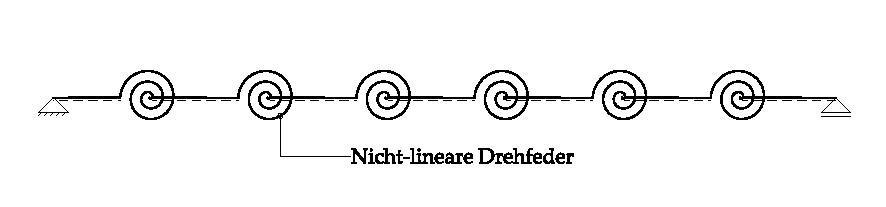
\includegraphics{index_files/mediabag/../imgs/Modell_Drehfeder.pdf}

}

\caption{\label{fig-modell_drehfeder}Modellierung als biegesteife Stäbe
gekoppelt mit Drehfedern}

\end{figure}%

Mit der Wahl der entsprechenden Federcharakteristiken stellen sich so
die passenden Resultate ein. Die Anwendung des Modells an
experimentellen Versuchen wird in den folgenden Kapiteln aufgegriffen.
Es lässt sich vorweggreifen, dass die Wahl der Federcharakteristik die
Krux des Systems darstellt.

Alternativ zur Modellierung mittels Drehfedern lässt sich das Verhalten
der Drehfeder mit einem Wegfederpaar abbilden. Dies erlaubt eine
Modellierung mittels den nicht-linearen Fachwerksstäben der Software
Statik-9 der Cubus AG. Dieser Ansatz wird lediglich im
Einführungsbeispiel berücksichtigt.

\begin{figure}[H]

\centering{

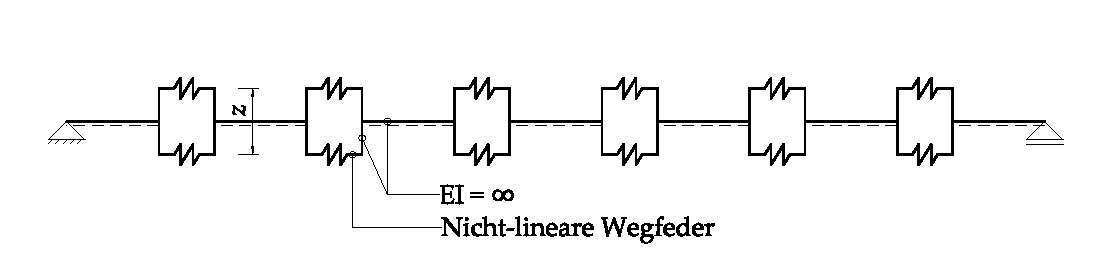
\includegraphics{index_files/mediabag/../imgs/Modell_Wegfeder.pdf}

}

\caption{\label{fig-modell_wegfeder}Modellierung als biegesteife Stäbe
gekoppelt mit einem Wegfederpaar}

\end{figure}%

\bookmarksetup{startatroot}

\chapter{Einführungsbeispiel}\label{einfuxfchrungsbeispiel}

Um das allgemeine Verständnis der Modellierung zu fördern, wird mit
einem Einführungsbeispiel gestartet. Das Beispiel verfolgt das Ziel, das
nicht-lineare Verformungsverhalten des Modells zu plausibilisieren. Es
gilt zu verstehen, wie das System in einer Stabstatik-Software zu
modellieren ist, um die gewünschten Ergebnisse zu erhalten.

Dazu werden die Verformungen des fiktiven Beispiels analytisch mittels
der Arbeitsgleichung, sowie numerisch mit der Stabstatik-Software
ermittelt. Das statische System ist in Abbildung~\ref{fig-kragarm-feder}
aufgezeigt. Das Beispiel ist mit einer Drehfeder versehen, welche eine
nicht-lineare Federcharakteristik aufweist. Es werden zwei Laststufen
betrachtet. Diese sind entsprechend gewählt, dass das nicht-lineare
Verhalten der Drehfeder zu tragen kommt.

\begin{figure}[H]

\centering{

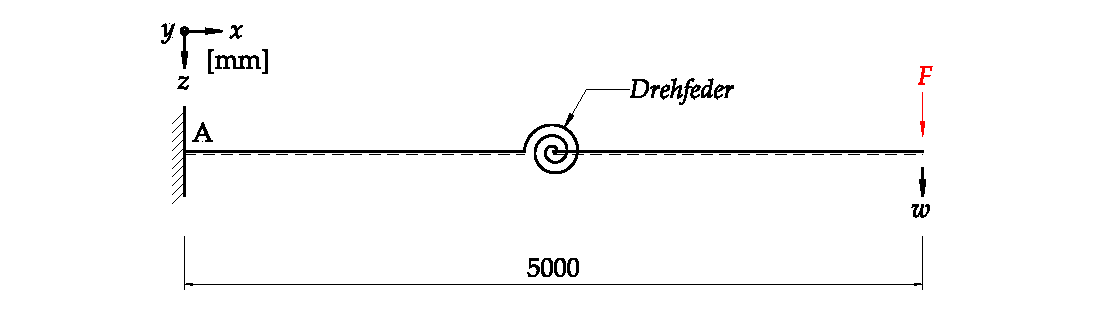
\includegraphics{index_files/mediabag/../imgs/Kragarm_system_Feder.pdf}

}

\caption{\label{fig-kragarm-feder}Statisches System des Kragarms}

\end{figure}%

Die folgenden Parameter fliessen in die Berechnungen ein. Beschrieben
sind die Abmessungen und Materialeigenschaften, sowie die beiden
Laststufen \(F_1\) und \(F_2\), wie auch die Federsteifigkeiten
\(k_{\varphi1}\) und \(k_{\varphi2}\).

$$
\begin{aligned}
E &= 10000.0\ \frac{\mathrm{N}}{\mathrm{mm}^{2}} \; 
 &F_{1} &= -10000.0\ \mathrm{N} \; 
 &F_{2} &= -21500.0\ \mathrm{N} \; 
\\[12pt]
 h &= 400.0\ \mathrm{mm} \; 
 &k_{\varphi_{1}} &= 100000.0\ \frac{\mathrm{N} \cdot \mathrm{m}}{\mathrm{rad}} \; 
 &k_{\varphi_{2}} &= 10000.0\ \frac{\mathrm{N} \cdot \mathrm{m}}{\mathrm{rad}} \; 
\\[12pt]
 L &= 5.0\ \mathrm{m} \; 
 &z &= 400.0\ \mathrm{mm} \; 
 &b &= 200.0\ \mathrm{mm} \; 
\\[12pt]
\end{aligned}
$$

Der Rechteckquerschnitt ist in Abbildung~\ref{fig-qs-kragarm}
aufgezeigt, dieser gilt für den gesamten Kragarm. Dieser dient lediglich
zur Bestimmung der Biegesteifigkeit.

\begin{figure}[H]

\centering{

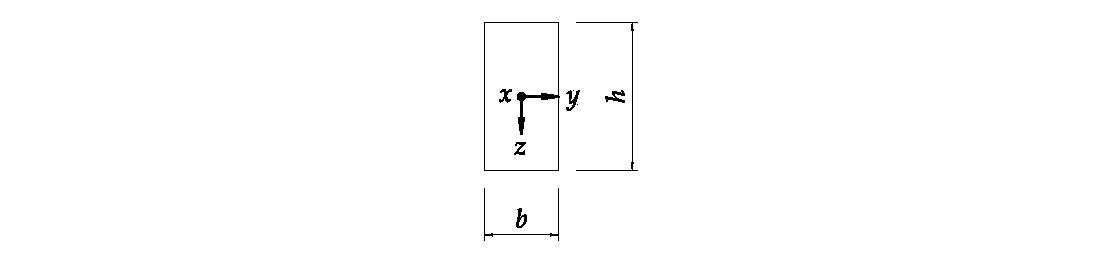
\includegraphics{index_files/mediabag/../imgs/Kragarm_querschnitt.pdf}

}

\caption{\label{fig-qs-kragarm}Fiktiver Querschnitt des Kragarms mit
durchwegs linear-elastischem Materialverhalten}

\end{figure}%

Die entsprechende Drehfedercharakteristik ist in
Abbildung~\ref{fig-springcharacteristic} zu sehen. Das Bilineare
Verhalten gilt für positive und negative Biegemomente um die
\(Y\)-Achse.

\begin{figure}[H]

\centering{

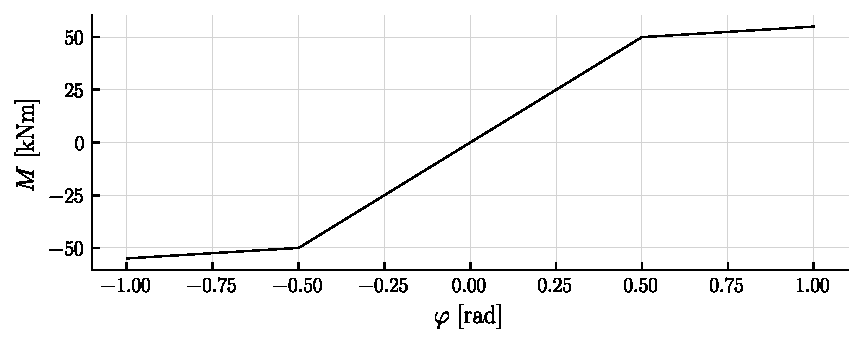
\includegraphics{index_files/mediabag/04_Kragarm_files/figure-pdf/fig-springcharacteristic-output-1.pdf}

}

\caption{\label{fig-springcharacteristic}Charakteristik der Drehfeder}

\end{figure}%

\section{Biegeverformung}\label{biegeverformung}

Zunächst werden die Biegeverformungen mittels der Differentialgleichung
für reine Biegeträger ermittelt. Dabei wird die Drehfeder
vernachlässigt. Das statische System, gezeigt in
Abbildung~\ref{fig-kragarm-sys} führt zu den Zustandslinien der
Schnittgrössen in der Abbildung~\ref{fig-skkragarmreal}.

\begin{figure}[H]

\centering{

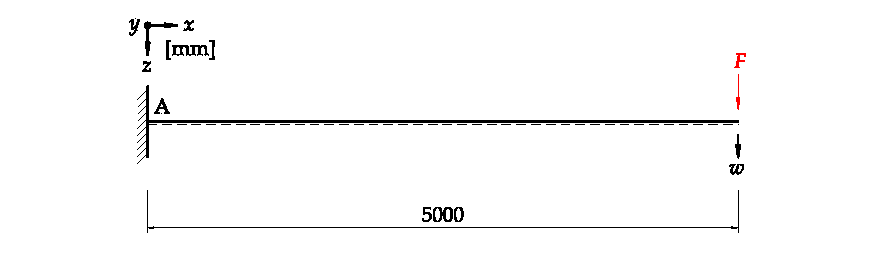
\includegraphics{index_files/mediabag/../imgs/Kragarm_System.pdf}

}

\caption{\label{fig-kragarm-sys}Statisches System des Kragarms}

\end{figure}%

\begin{figure}[H]

\centering{

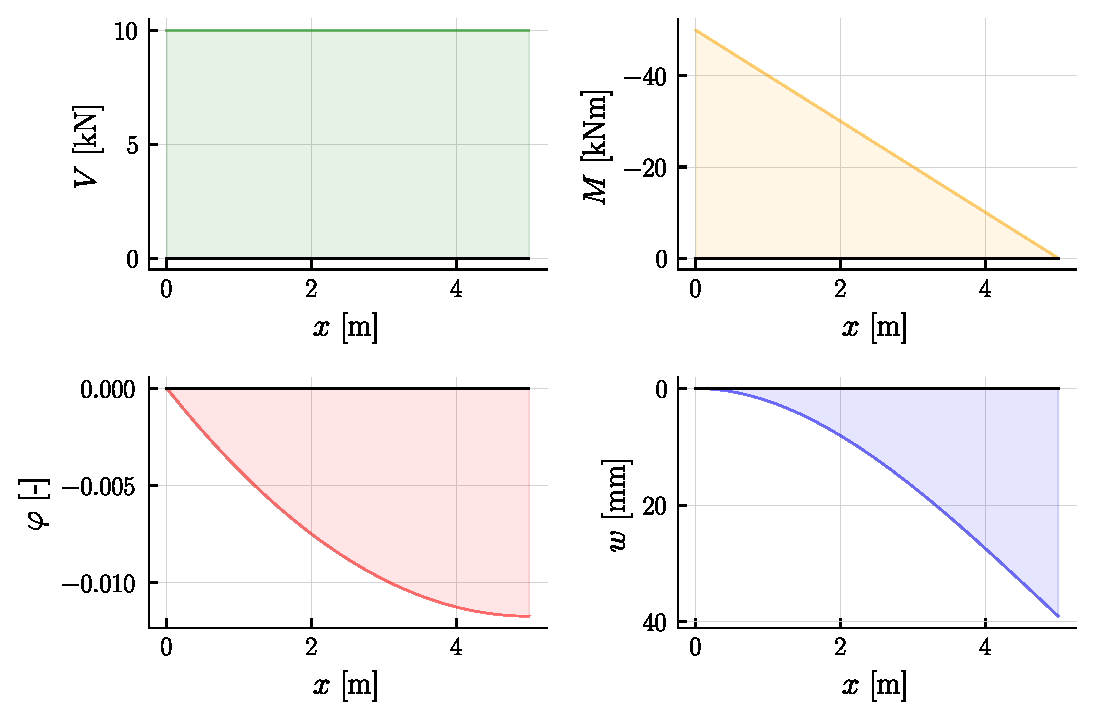
\includegraphics{index_files/mediabag/04_Kragarm_files/figure-pdf/fig-skkragarmreal-output-1.pdf}

}

\caption{\label{fig-skkragarmreal}Schnittkräfte des Systems aus
Abbildung~\ref{fig-kragarm-sys} für die Last \(F_1\)}

\end{figure}%

Die maximale Verformung am Endpunkt des Kragarms beträgt:

$$
\begin{aligned}
w_{EI_{F1}} &= 39.1\ \mathrm{mm} \;
\end{aligned}
$$

Das analoge Vorgehen führt für die Laststufe \(F_2\) zu den
Zustandslinien der Schnittgrössen gemäss der
Abbildung~\ref{fig-skkragarmreal_high}.

\begin{figure}[H]

\centering{

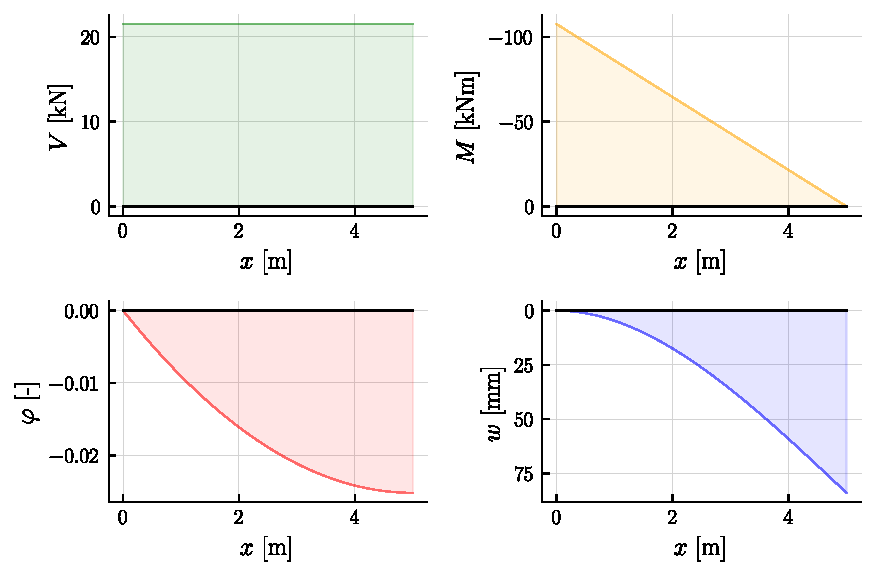
\includegraphics{index_files/mediabag/04_Kragarm_files/figure-pdf/fig-skkragarmreal_high-output-1.pdf}

}

\caption{\label{fig-skkragarmreal_high}Schnittkräfte des Systems aus
Abbildung~\ref{fig-kragarm-sys} für die Last \(F2\)}

\end{figure}%

Da ein durchwegs linear-elastisches Biegeverhalten vorausgesetzt wird,
entspricht der Faktor der Erhöhung des Verformung dem Quotient der
beiden Laststufen.

\[
\frac{w_{EI_{F2}}}{w_{EI_{F1}}} = \frac{F_2}{F_1}
\]

Dabei entspricht die maximale Biegeverformung am Ende des Kragarms:

$$
\begin{aligned}
w_{EI_{F2}} &= 84.0\ \mathrm{mm} \;
\end{aligned}
$$

\section{Verformung der Drehfeder}\label{verformung-der-drehfeder}

Zur Bestimmung der Verformung am Ende des Kragarms des Systems mit der
Drehfeder wird die Arbeitsgleichung angewendet. Dazu wird an einem
virtuellen System eine Einzellast eingeführt, an der Stelle an dem die
Verformung bestimmt werden soll. Dargestellt ist dies in
Abbildung~\ref{fig-kragarm-sys-virtuell}.

\begin{figure}[H]

\centering{

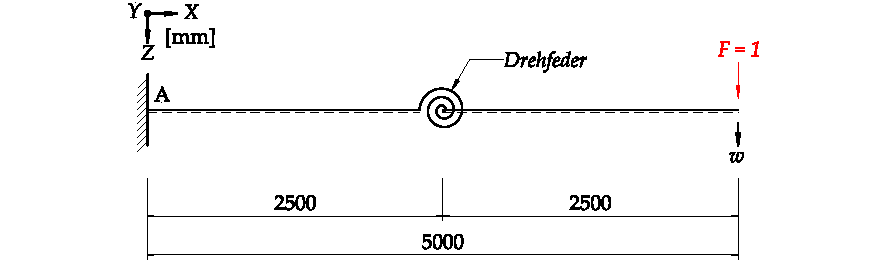
\includegraphics{index_files/mediabag/../imgs/Kragarm_system_feder_virtuell.pdf}

}

\caption{\label{fig-kragarm-sys-virtuell}Statisches System des Kragarms
im virtuellen Kräftezustand}

\end{figure}%

Die entsprechenden Verläufe der Querkraft und des Biegemoments zeigt die
Abbildung~\ref{fig-sk-kragarm-virtuell} für das virtuelle System.

\begin{figure}[H]

\centering{

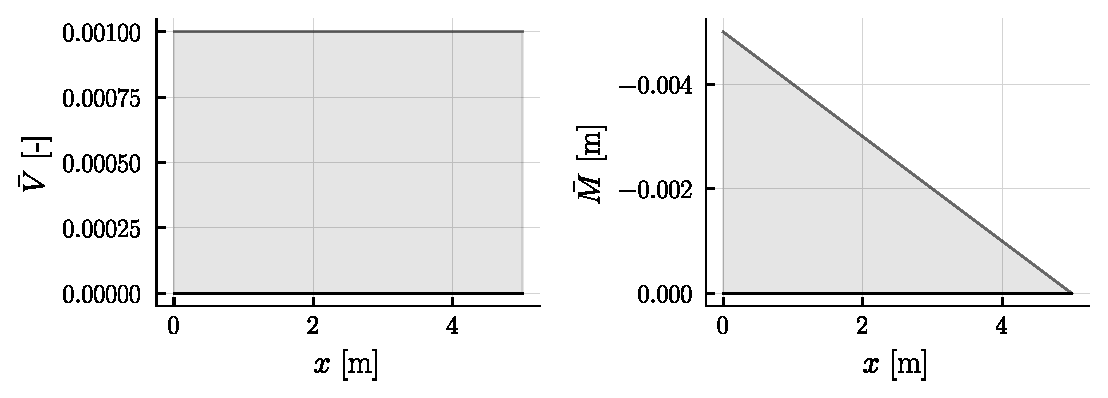
\includegraphics{index_files/mediabag/04_Kragarm_files/figure-pdf/fig-sk-kragarm-virtuell-output-1.pdf}

}

\caption{\label{fig-sk-kragarm-virtuell}Schnittkräfte des virtuellen
Systems aus Abbildung~\ref{fig-kragarm-sys-virtuell}}

\end{figure}%

Die Verformung der Drehfeder kann abschliessend mit der folgenden
Gleichung bestimmt werden.

\[
w_{\varphi} = \bar{M} \frac{M}{k_\varphi} = \bar{M} \varphi
\]

Die Verdrehung lässt sich aus der Federcharakteristik mit dem
Biegemoment an der Stelle der Drehfeder bestimmen. Die
Abbildung~\ref{fig-feder-force} zeigt die Position der Laststufen im
Diagramm.

\begin{figure}[H]

\centering{

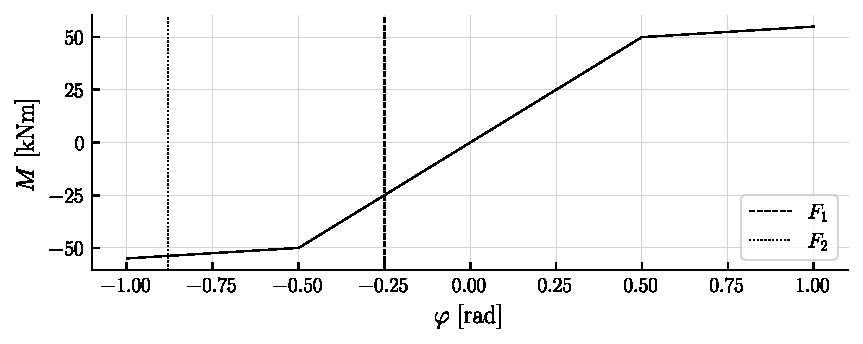
\includegraphics{index_files/mediabag/04_Kragarm_files/figure-pdf/fig-feder-force-output-1.pdf}

}

\caption{\label{fig-feder-force}Charakteristik der Drehfeder mit
Bestimmung der Verdrehung anhand der Laststufen}

\end{figure}%

Angewendet auf das System der Abbildung~\ref{fig-kragarm-feder} folgen
für die beiden Laststufen die Deformationen der Drehfeder zu:

$$
\begin{aligned}
w_{\varphi_{F1}} &= 625.0\ \mathrm{mm} \; 
 &w_{\varphi_{F2}} &= 2201.3\ \mathrm{mm} \;
\end{aligned}
$$

Dazu gilt es den Anteil aus der Biegeverformung zu addieren. Die totale
Verformung folgt zu:

$$
\begin{aligned}
w_{F1} &= w_{\varphi_{F1}} + w_{EI_{F1}}  = 625.0\ \mathrm{mm} + 39.1\ \mathrm{mm} &= 664.1\ \mathrm{mm}  
\\[12pt]
w_{F2} &= w_{\varphi_{F2}} + w_{EI_{F2}}  = 2201.3\ \mathrm{mm} + 84.0\ \mathrm{mm} &= 2285.2\ \mathrm{mm}  
\end{aligned}
$$

\section{Stabstatikmodell}\label{stabstatikmodell}

Das statische System, gemäss Abbildung~\ref{fig-kragarm-feder}, wird
mittels der Statiksoftware AxisVM X7 modelliert. Dazu wird die Drehfeder
als Federelement modelliert und in der \(YY\)-Dimension mit der
Federcharakteristik ergänzt. Die angeschlossenen Stäbe sind mit
entsprechendem Querschnitt und der entsprechenden Biegesteifigkeit
modelliert.

Die Deformationen in \(Z\)-Richtung sind in
Abbildung~\ref{fig-kragarm-drehfeder-10} und
Abbildung~\ref{fig-kragarm-drehfeder-215}

\begin{figure}[H]

\centering{

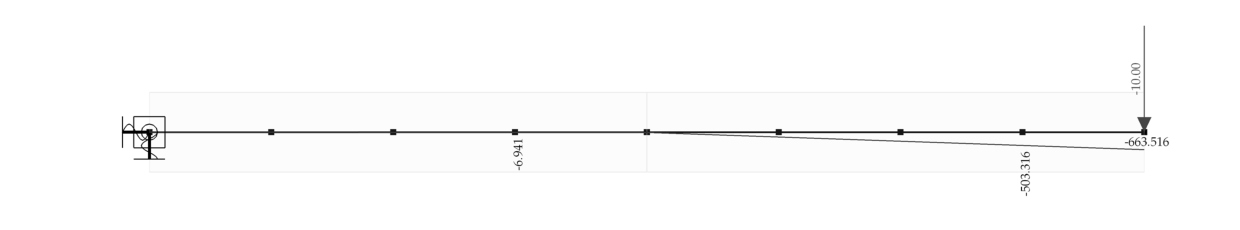
\includegraphics{index_files/mediabag/../imgs/Kragarm_drehfeder_10.pdf}

}

\caption{\label{fig-kragarm-drehfeder-10}Verformungen in \(z\) für
\(F_1\) aus AxisVM mit Drehfedermodell}

\end{figure}%

Das Modell liefert für die erste Laststufe die Gesamtverformung von:

\[
w_{1,tot,F1} = 663.5 \text{mm}
\]

\begin{figure}[H]

\centering{

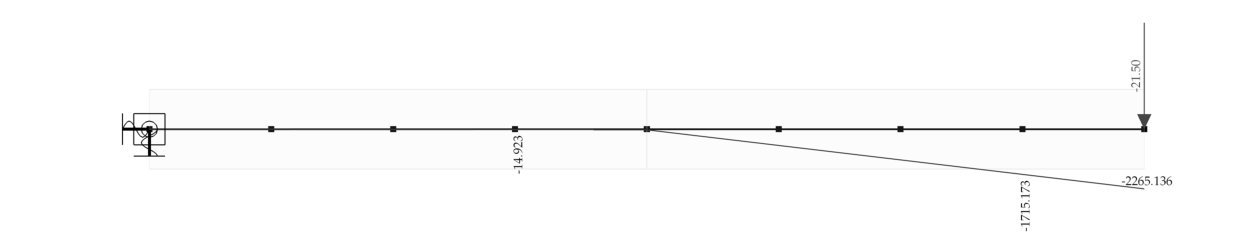
\includegraphics{index_files/mediabag/../imgs/Kragarm_drehfeder_215.pdf}

}

\caption{\label{fig-kragarm-drehfeder-215}Verformungen in \(z\) für
\(F_2\) aus AxisVM mit Drehfedermodell}

\end{figure}%

So wie für die zweite Laststufe folgt die Gesamtverformung zu:

\[
w_{1,tot,F2} = 2265.1 \text{mm}
\]

Das Modell liefert die annähernd gleichen Resultate wie die
Handrechnung. Die Genauigkeit ist zufriedenstellend.

\subsection{Modellierungsalternative
Wegfeder}\label{modellierungsalternative-wegfeder}

Wie bereits in Kapitel~\ref{sec-modellvorstellung} aufgezeigt, lässt
sich das Verhalten der Drehfeder mit einem Wegfederpaar abbilden. Dazu
wird in einem ersten Schritt die Drehfedercharakteristik in eine
Wegfedercharakteristik umgerechnet. Als Grundlage dient die Modellierung
gemäss Abbildung~\ref{fig-verdrehung_verformung}. Die Abbildung zeigt
die kinematische Relation eines reinen Biegeelements.

\begin{figure}[H]

\centering{

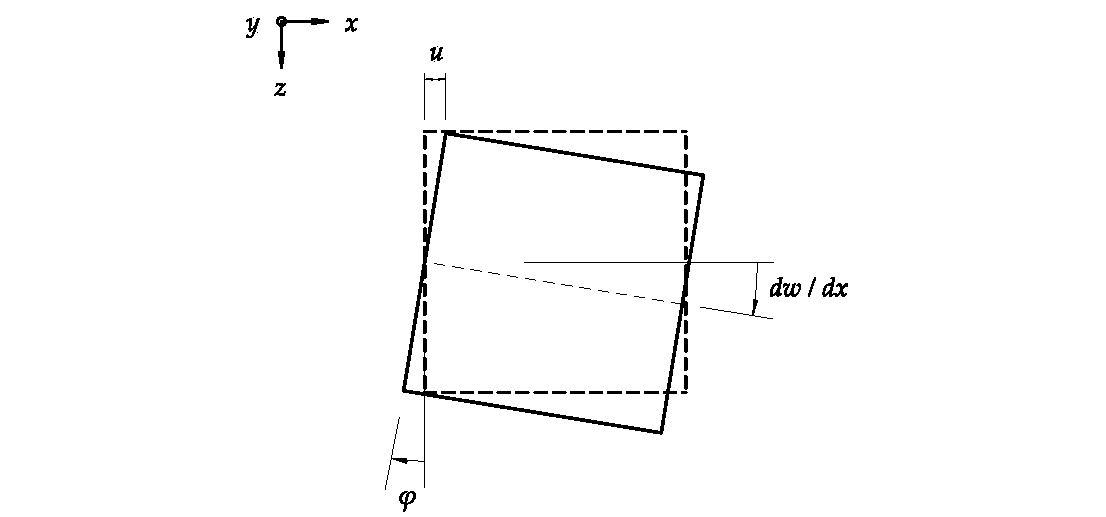
\includegraphics{index_files/mediabag/../imgs/Skizze_Verdrehung_Verformung.pdf}

}

\caption{\label{fig-verdrehung_verformung}Kinematische Relation eines
reinen Biegeelements}

\end{figure}%

Mittels den folgenden Gleichungen lässt sich so die
Wegfedercharakteristik bestimmen. Der Abstand zwischen dem Wegfederpaar
wird mit \(z\) beschrieben.

\[
F = \frac{M}{z}
\]

\[
u = \frac{\tan(\varphi) \cdot z}{2} \simeq \frac{\varphi \cdot z}{2}
\]

Durch die Berücksichtigung der trigonometrischen Funktion ist der
Verlauf nicht exakt bilinear. Eine Approximation mit einem bilinearen
Verlauf führt zu beträchtlichen Abweichungen im Bereich der zweiten
Laststufe \(F_2\). Dies ist auf die geringe Neigung, bzw.
\(k_{\varphi_2}\) der Drehfedercharakteristik im oberen Lastniveau
zurückzuführen.

Die umgerechnete Wegfedercharakteristik ist in
Abbildung~\ref{fig-wegfeder-force} aufgezeigt.

\begin{figure}[H]

\centering{

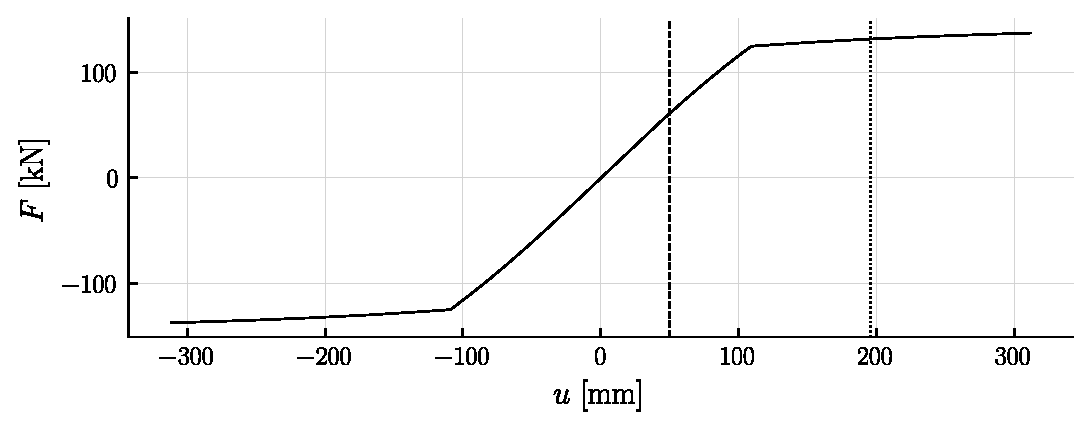
\includegraphics{index_files/mediabag/04_Kragarm_files/figure-pdf/fig-wegfeder-force-output-1.pdf}

}

\caption{\label{fig-wegfeder-force}Charakteristik der Wegfeder}

\end{figure}%

Die Resultate mit dem Modell sind in der Abbildung~\ref{fig-f1-wegfeder}
und Abbildung~\ref{fig-f2-wegfeder} gezeigt.

\begin{figure}[H]

\centering{

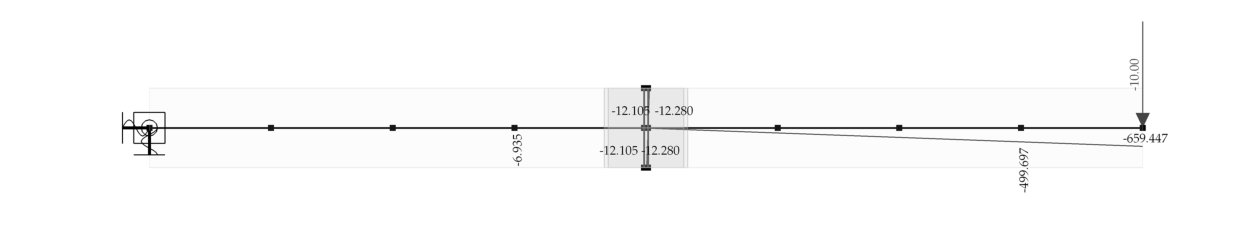
\includegraphics{index_files/mediabag/../imgs/Kragarm_wegfeder_10.pdf}

}

\caption{\label{fig-f1-wegfeder}Verformungen in \(z\) für \(F_1\) aus
AxisVM mit Wegfedermodell}

\end{figure}%

Die maximale Verformung in \(Z\)-Richtung ist für die Laststufe \(1\):

\[
w_{1,tot,F1} = 655 \text{mm}
\]

Und für die Laststufe \(2\):

\[
w_{1,tot,F2} = 2137.8 \text{mm}
\]

Hier zeigt sich eine Abweichung. Diese lässt sich auf die numerisch
approximierte Modellierung der Wegfederbeziehung zurückführen.

\begin{figure}[H]

\centering{

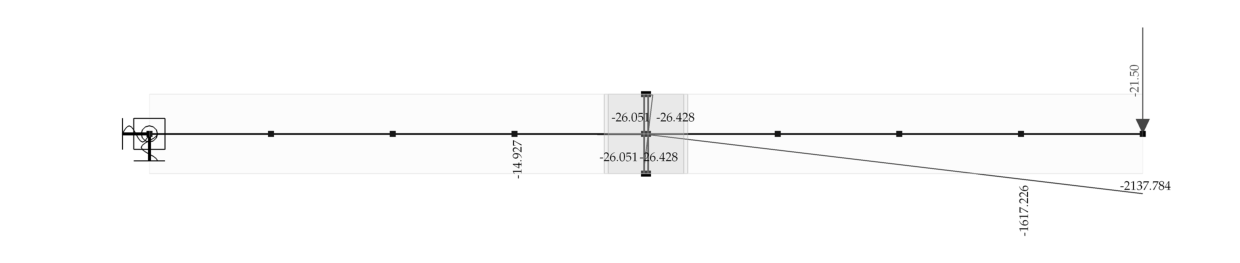
\includegraphics{index_files/mediabag/../imgs/Kragarm_wegfeder_215.pdf}

}

\caption{\label{fig-f2-wegfeder}Verformungen in \(z\) für \(F_2\) aus
AxisVM mit Wegfedermodell}

\end{figure}%

\section{Zusammenfassung}\label{zusammenfassung}

Das Einführungsbeispiel zeigt die Präzision der Modellierung mittels dem
Drehfedermodell. Sowie ermöglicht die simple Aufgabenstellung das
Nachvollziehen der Resultate.

\bookmarksetup{startatroot}

\chapter{Modellverifizierung}\label{sec-verifizierung}

Diese Kapitel beschreibt die Anwendung des Drehfedermodells auf die
beiden Versuche der Vorarbeit {[}\citeproc{ref-gitz_ansatze_2024}{1}{]}.
Dabei sind lediglich die relevanten Grundlagen der Versuche aufgezeigt.
Detaillierte Beschriebe sind aus
{[}\citeproc{ref-gitz_ansatze_2024}{1}{]} und verwiesener Literatur zu
entnehmen.

Es wird erwartet, dass das Drehfedermodell die Biegeverformungen
vollumfänglich beschreibt, sofern die Momenten-Verdrehungs-Beziehung
präzise bestimmt werden kann. Zusätzlich ermöglicht das Modell die
Beschreibung der Schubverformungen. Dies bedingt eine entsprechende
Ermittlung der Steifigkeit in Richtung der erwarteten Schubverformungen.
Abschliessend wird ein Ansatz gezeigt um Längszugkräfte infolge
Querkraft mit dem Modell abzubilden.

\section{Dreipunktbiegeversuch}\label{dreipunktbiegeversuch}

Der Dreipunktbiegeversuch ist der dritte Versuch der Serie A in der
zweiten Versuchsanordnung aus
{[}\citeproc{ref-jager_versuche_2006}{2}{]}, kurz betitelt mit A3V2. Der
Versuchsaufbau ist in der Abbildung~\ref{fig-anordnung_a3v2} gezeigt. An
der Stelle \(A\) wird der Plattenstreifen bis zum Versagen belastet.
Gemessen sind die Verformungen an der Stelle der Lasteinleitung nach dem
Einbringen des Trägers auf dem Versuchsstand.

\begin{figure}[H]

\centering{

\includegraphics{index_files/mediabag/../imgs/versuchsanordnung_A3V2.pdf}

}

\caption{\label{fig-anordnung_a3v2}Versuchsanordnung des Versuchs A3V2,
Zeichnung entnommen aus {[}\citeproc{ref-jager_versuche_2006}{2}{]}}

\end{figure}%

Das Bewehrungslayout ist in der Abbildung~\ref{fig-bewehrung_a3v2}
aufgezeigt. Der Plattenstreifen ist mit einer durchgehenden
Längsbewehrung in der Zugzone bewehrt. Verankert ist die Längsbewehrung
mit angeschweissten Platten. Die Schubdübel sind nicht durchgängig
verlegt.

\begin{figure}[H]

\centering{

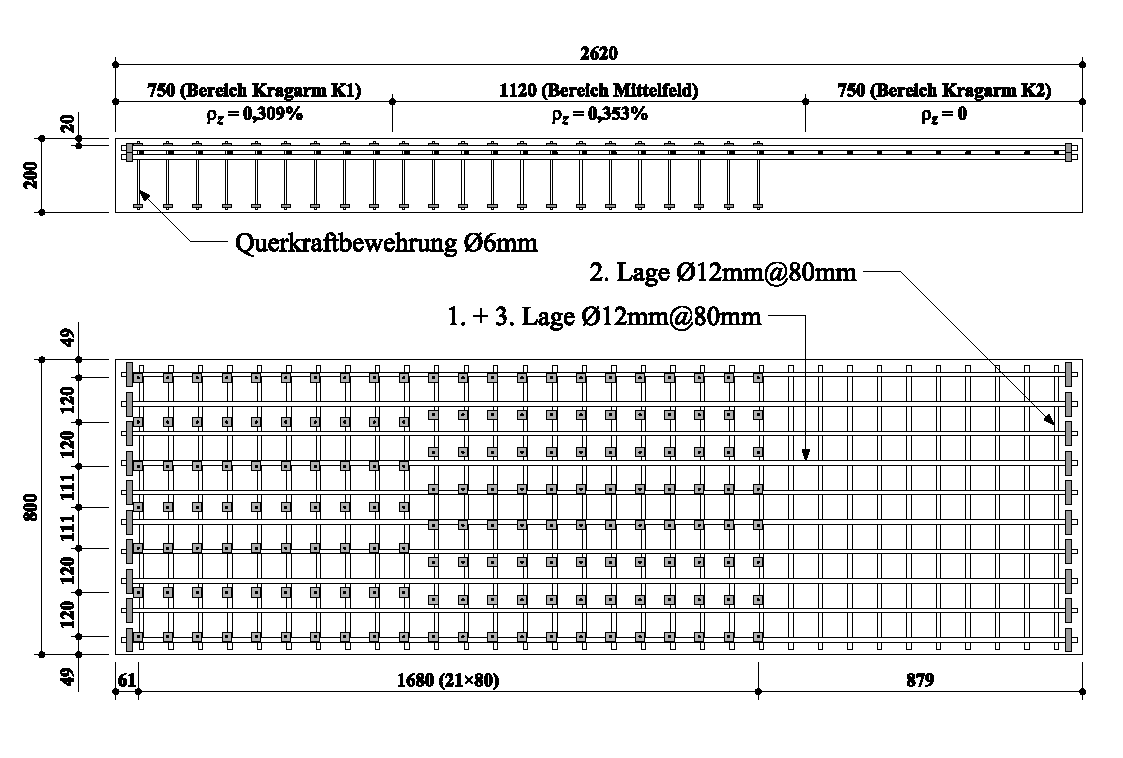
\includegraphics{index_files/mediabag/../imgs/bewehrung_a3v2.pdf}

}

\caption{\label{fig-bewehrung_a3v2}Bewehrunslayout des Versuchs A3V2,
Zeichnung entnommen aus {[}\citeproc{ref-jager_versuche_2006}{2}{]}}

\end{figure}%

Die Abbildung~\ref{fig-qs_a3v2} zeigt das Bewehrungslayout in
querrichtung, sowie entsprechende Abmessungen des Plattenstreifens.

\begin{figure}[H]

\centering{

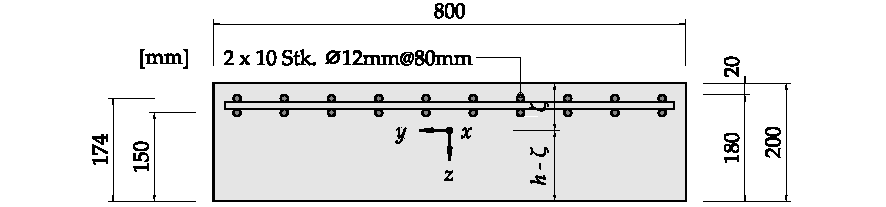
\includegraphics{index_files/mediabag/../imgs/QS_Versuch_A3.pdf}

}

\caption{\label{fig-qs_a3v2}Querschnitt des Versuchs A3V2, Zeichnung
entnommen aus {[}\citeproc{ref-gitz_ansatze_2024}{1}{]}}

\end{figure}%

\subsection{Modellierung}\label{modellierung}

In diesem Abschnitt wird die Modellbildung beschrieben. Das Ziel ist es
das Verhalten des Versuchskörpers mit einem möglichst simplen Modell
abzubilden. Das statische System des Versuchs ist in
Abbildung~\ref{fig-system_a3v2} dargestellt. Das Eigengewicht wird
vernachlässigt, da die Verformungsmessungen nach dem Einbau des Versuchs
beginnen, bzw. erst bei Belastungsbeginn mit der Einzellast.

\begin{figure}[H]

\centering{

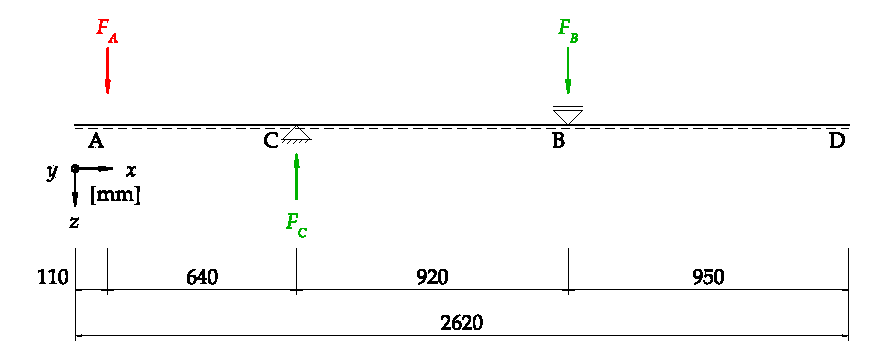
\includegraphics{index_files/mediabag/../imgs/A3V2_system.pdf}

}

\caption{\label{fig-system_a3v2}Statisches System des Versuchs A3V2}

\end{figure}%

Die Auflagerbreiten werden vernachlässigt, bzw. wird der Plattenstreifen
punktgestützt modelliert. Auf die Darstellung der biegesteifen Elemente
mit Endgelenken wird verzichtet. Diese sind in einem Abstand von \(10\)
mm entlang der Stabachse verteilt.

$$
\begin{aligned}
l_{E} &= 10.0\ \mathrm{mm} \; \;\textrm{(Elementlänge des Biegesteifen Stabs)}
\end{aligned}
$$

Der Einfluss der Elementlänge wurde mittels einer Sensitivitätsanalyse
ermittelt. Eine feinere Stabunterteilung resultiert zu keiner
signifikanten Steigerung der Genauigkeit.

\subsubsection{Biegeverformungen}\label{biegeverformungen}

Um das Biegeverhalten passend zu beschreiben gilt es eine entsprechende
Drehfedercharakteristik zu bestimmen. Dazu wird anhand einer
Querschnittsanalyse eine Momenten-Krümmungs-Beziehung ermittelt. Durch
Multiplikation der Krümmung mit der Elementlänge resultiert eine
Momenten-Verdrehungs-Beziehung, sprich eine Drehfedercharakteristik. Es
wird von einem Bilinearen Spannungs-Dehnungs-Verhalten des Betonstahls,
sowie von einer linear-elastischen ideal plastischen
Spannungs-Dehnungs-Beziehung des Betons mit Berücksichtigung der
Zugfestigkeit ausgegangen. Für den Querschnitt ist die nicht-lineare
Beziehung in der Abbildung~\ref{fig-mchi_a3v2} gezeigt. Detaillierte
Berechnungen sind in der Vorarbeit
{[}\citeproc{ref-gitz_ansatze_2024}{1}{]} zu finden.

\begin{figure}[H]

\centering{

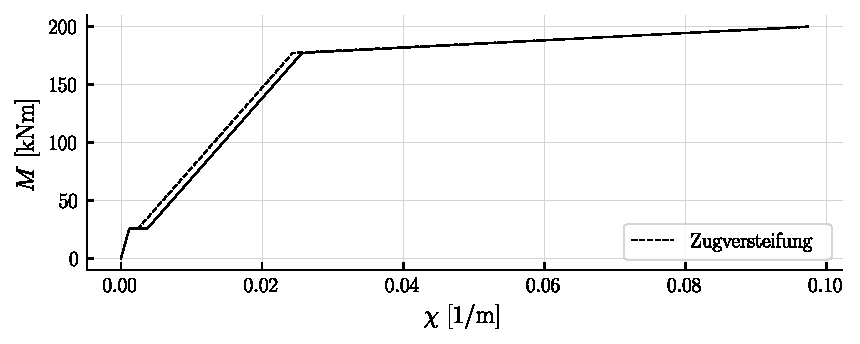
\includegraphics{index_files/mediabag/05_Versuchsnachrechnung_VM1_files/figure-pdf/fig-mchi_a3v2-output-1.pdf}

}

\caption{\label{fig-mchi_a3v2}Momenten-Krümmungs-Beziehung des
Dreipunktbiegeversuchs, übernommen aus
{[}\citeproc{ref-gitz_ansatze_2024}{1}{]}}

\end{figure}%

Die Momenten-Krümmungs-Beziehung zeigt einen Bereich des ungerissenen
Querschnitts, gefolgt vom gerissenen Bereich, welcher die Zugversteifung
mit dem Ansatz nach Marti basierend auf dem Zuggurtmodell
berücksichtigt. Beim Erreichen der Fliessspannung in den
Bewehrungsstäben flacht die Beziehung deutlich ab.

Die daraus resultierende Momenten-Verdrehungs-Beziehung ist in der
Abbildung~\ref{fig-mphi_a3v2} aufgezeigt. Diese ist den Stabendgelenken
als Verdrehung in globaler \(Y\)-Richtung, gemäss
Abbildung~\ref{fig-system_a3v2}, zu hinterlegen.

\begin{figure}[H]

\centering{

\includegraphics{index_files/mediabag/05_Versuchsnachrechnung_VM1_files/figure-pdf/fig-mphi_a3v2-output-1.pdf}

}

\caption{\label{fig-mphi_a3v2}Momenten-Verdrehungs-Beziehung des
Dreipunktbiegeversuchs}

\end{figure}%

\subsubsection{Schubverformungen}\label{schubverformungen}

Um die Schubverformungen im Modell abzubilden, gilt es eine
Wegfedercharakteristik in globaler \(Z\)-Richtung, entsprechend dem
Koordinatensystem aus Abbildung~\ref{fig-system_a3v2}, zu bestimmen. Als
Grundlage zur Modellierung der Schubverformungen dient das
Spannungsfeld-Modell in Abbildung~\ref{fig-spannungsfelder_a3v2}. Dabei
wird vorausgesetzt, dass sämtliche Dehnung des Systems in vertikaler
Richtung lediglich aus der Stabdehnung der Schubbewehrung erfolgt.

\begin{figure}[H]

\centering{

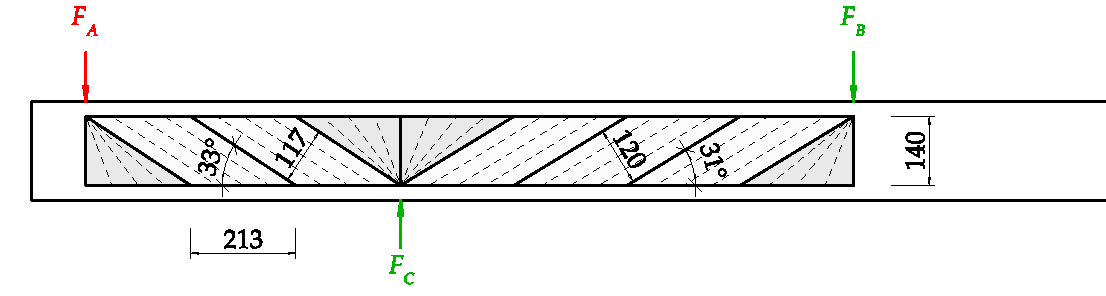
\includegraphics{index_files/mediabag/../imgs/Spannungsfelder_flach.pdf}

}

\caption{\label{fig-spannungsfelder_a3v2}Einteilung in Spannungsfelder
des Versuchs A3V2, Zeichnung entnommen aus
{[}\citeproc{ref-gitz_ansatze_2024}{1}{]}}

\end{figure}%

Durch die Einteilung in Spannungsfelder kann die Anzahl an mitwirkenden
Schubdübeln bestimmt werden. Mit der Querschnittsfläche der mitwirkenden
Dübel kann mittels dem nicht-linearen Spannungs-Dehnungs-Verhalten,
gezeigt in der Abbildung~\ref{fig-sigma-eps-a3v2}, die Kraftkomponente
ermittelt werden. Die Verformung wird mittels Multiplikation der
Dehnungen aus der Spannungs-Dehnungs-Beziehung mit dem Hebelarm der
inneren Kräfte bestimmt. Dies führt zu einer
Kraft-Verformungs-Beziehung, sprich einer Wegfedercharakteristik für das
gesamte Spannungsfeld.

\[
\gamma_{E} = \frac{z \cdot \cot(\theta)}{n_{E}}
\]

\(n_{E}\) steht für die Anzahl steifer Stabelemente

Abschliessend wird die Verformung um den Faktor gemäss der folgenden
Gleichung reduziert, bzw. die Steifigkeit der Feder um diesen Faktor
erhöht. Die daraus resultierende Wegfedercharakteristik ist den
Stabendgelenken zu hinterlegen.

\begin{figure}[H]

\centering{

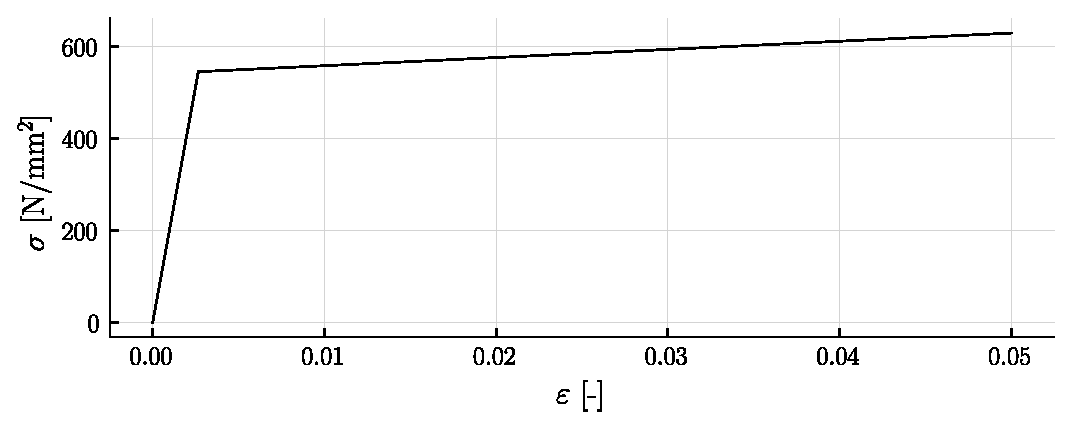
\includegraphics{index_files/mediabag/05_Versuchsnachrechnung_VM1_files/figure-pdf/fig-sigma-eps-a3v2-output-1.pdf}

}

\caption{\label{fig-sigma-eps-a3v2}Spannungs-Dehnungs-Beziehung der
Schubbewehrung, übernommen aus
{[}\citeproc{ref-gitz_ansatze_2024}{1}{]}}

\end{figure}%

Folgend sind die Parameter zur Bestimmung der Wegfedercharakteristik in
vertikaler Richtung gezeigt. Der gewählte Neigungswinkel der
Spannungsfelder \(\theta_{c3}\) gilt grundsätzlich nur im Bruchzustand.
Als Approximation wird die daraus bestimmte Wegfedercharakteristik für
sämtliche Laststufen angesetzt. Dies führt zu Abweichungen des
Verformungsverhalten im Lastniveau unterhalb der Traglast. Da der
Einfluss der Schubverformungen jedoch gering ist, ist diese
Vereinfachung unproblematisch.

$$
\begin{aligned}
\oslash_{sw_{A3V2}} &= 6.0\ \mathrm{mm} \; 
 &S_{sw_{A3V2}} &= 80.0\ \mathrm{mm} \; 
 &b_{w_{A3V2}} &= 800.0\ \mathrm{mm} \; 
\\[12pt]
 E_{sw_{A3V2}} &= 205000.0\ \frac{\mathrm{N}}{\mathrm{mm}^{2}} \; 
 &z_{A3V2} &= 140.0\ \mathrm{mm} \; 
 &\theta_{c3_{A3V2}} &= 34.3\ \mathrm{°} \; 
\\[12pt]
 f_{su_{A3V2}} &= 630.0\ \frac{\mathrm{N}}{\mathrm{mm}^{2}} \;
\end{aligned}
$$

In einem ersten Schritt wird die Querschnittsfläche der Schubbewehrung
bestimmt. Gemäss der Abbildung~\ref{fig-bewehrung_a3v2} ist ersichtlich,
dass entlang der Plattenbreite \(7\) Schubdübel verlegt sind. Die
Querschnittsfläche für eine Dübelreihe folgt somit zu:

$$
\begin{aligned}
A_{sw_{A3V2}} &= 7 \cdot \left( \frac{ \oslash_{sw_{A3V2}} }{ 2 } \right) ^{ 2 } \cdot \pi \; 
\end{aligned}
$$

$$
\begin{aligned}
A_{sw_{A3V2}} &= 197.9\ \mathrm{mm}^{2} \;
\end{aligned}
$$

Wird diese nun über einen Meterstreifen verschmiert, so folgt:

$$
\begin{aligned}
a_{sw_{A3V2}} &= \frac{ A_{sw_{A3V2}} }{ S_{sw_{A3V2}} } \; 
\end{aligned}
$$

$$
\begin{aligned}
a_{sw_{A3V2}} &= 2474.0\ \frac{\mathrm{mm}^{2}}{\mathrm{m}} \;
\end{aligned}
$$

In einem nächsten Schritt wird der Querkraftwiderstand bestimmt. Dies
dient grundsätzlich zur Bestimmung des Neigungswinkel. Aus den
Versuchsergebnissen ist ersichtlich, dass der Plattenstreifen bei
\(320\) kN versagt. Somit muss ein Spannungsfeld gewählt werden, welches
einen Querkraftwiderstand entsprechend der Traglast liefert. Durch
Iteration dieser Gleichung wurde der Neigungswinkel \(\theta_{c3}\)
ermittelt.

$$
\begin{aligned}
V_{Rd_{A3V2}} &= a_{sw_{A3V2}} \cdot z_{A3V2} \cdot \frac{ f_{su_{A3V2}} }{ \tan \left( \theta_{c3_{A3V2}} \right) } \; 
\end{aligned}
$$

$$
\begin{aligned}
V_{Rd_{A3V2}} &= 319.9\ \mathrm{kN} \;
\end{aligned}
$$

Abschliessend gilt es den Reduktionsfaktor zu bestimmen:

$$
\begin{aligned}
\gamma_{E_{A3V2}} &= z_{A3V2} \cdot \frac{ 1 }{ \tan \left( \theta_{c3_{A3V2}} \right) } \cdot \frac{1} { l_{E} }  = 140\ \mathrm{mm} \cdot \frac{ 1 }{ \tan \left( 34\ \mathrm{°} \right) } \cdot \frac{1} { 10\ \mathrm{mm} } &= 21\  
\end{aligned}
$$

Die Abbildung~\ref{fig-wegfeder-schub-a3v2} zeigt das ermittelte
Kraft-Verformungs-Verhalten. Das Verhalten ist analog dem bilinearen
Spannungs-Dehnungs-Diagramm.

\begin{figure}[H]

\centering{

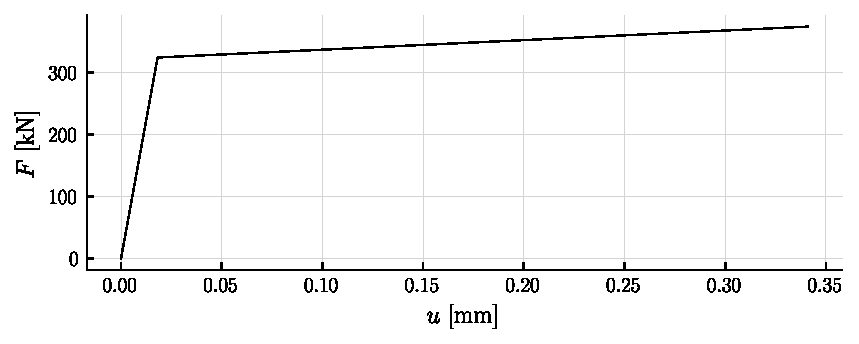
\includegraphics{index_files/mediabag/05_Versuchsnachrechnung_VM1_files/figure-pdf/fig-wegfeder-schub-a3v2-output-1.pdf}

}

\caption{\label{fig-wegfeder-schub-a3v2}Berechnete
Wegfedercharakteristik des Schubgelenks vom Versuch A3V2}

\end{figure}%

\subsection{Ergebnisse}\label{ergebnisse}

Mit den bestimmten Federcharakteristiken kann die Verformungslinie des
Systems ermittelt werden. Das Modell ist in der Lage, Biege- und
Schubverformungen zu beschreiben, basierend auf nicht-linearen
Eigenschaften. Die Abbildung~\ref{fig-fwa3v2} zeigt das
Last-Verformungs-Diagramm des Systems am Punkt \(w_1\). Gezeigt sind die
Resultate des Modells, mit und ohne Berücksichtigung der Zugversteifung,
sowie die gemessenen Versuchsresultate aus dem Versuchsbericht. Das
Modell beschreibt den Verformungsverlauf zufriedenstellend.

\begin{figure}[H]

\centering{

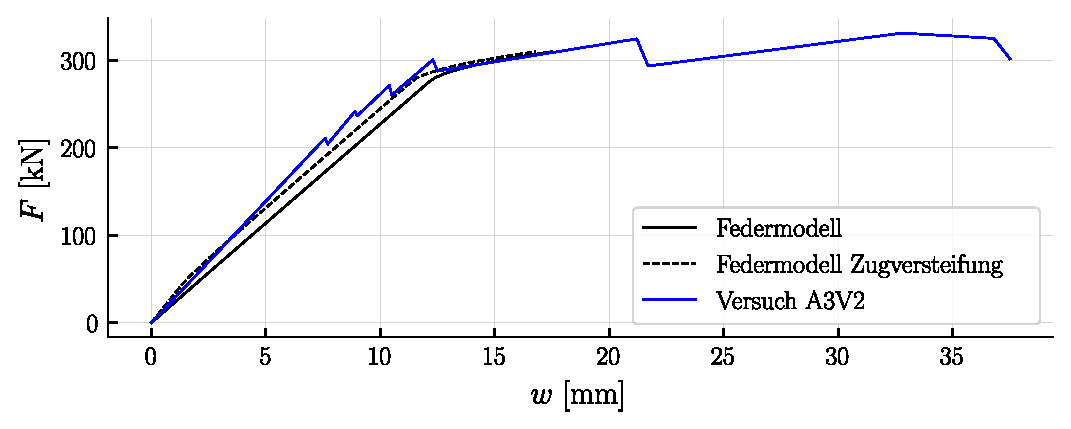
\includegraphics{index_files/mediabag/05_Versuchsnachrechnung_VM1_files/figure-pdf/fig-fwa3v2-output-1.pdf}

}

\caption{\label{fig-fwa3v2}Last-Verformungs-Verlauf am Punkt \(w_1\) mit
dem Federmodell und den Versuchsmessungen}

\end{figure}%

Der Verdrehungsverlauf in Abbildung~\ref{fig-phi-max-a3v2} lässt sich
ebenfalls direkt aus dem Modell exportieren. Durch die Ableitung des
Verlaufs resultiert der Krümmungsverlauf, dargestellt in
Abbildung~\ref{fig-chi-max-a3v2}.

\begin{figure}[H]

\centering{

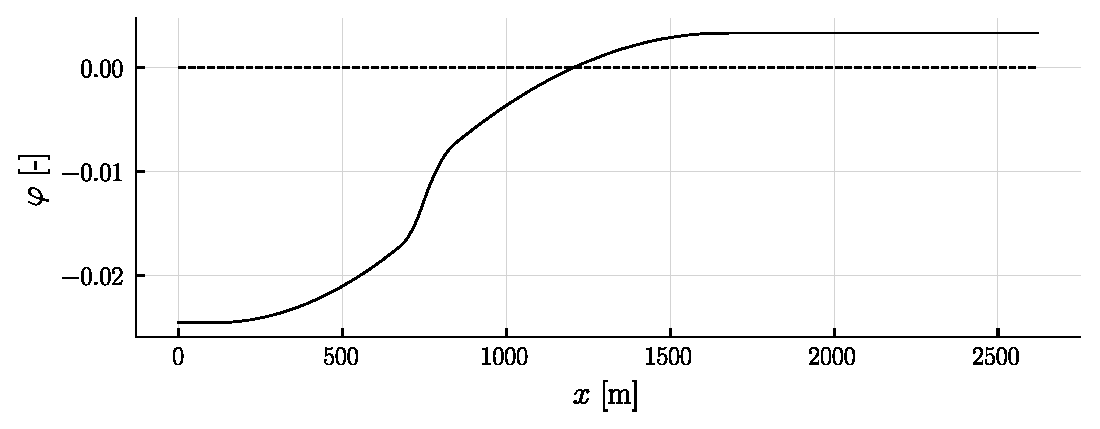
\includegraphics{index_files/mediabag/05_Versuchsnachrechnung_VM1_files/figure-pdf/fig-phi-max-a3v2-output-1.pdf}

}

\caption{\label{fig-phi-max-a3v2}Verdrehungsverlauf aus dem Federmodell
für die Höchstlast}

\end{figure}%

Der Krümmungsverlauf gibt Aufschluss über den Fliessbereich der
Bewehrung, bzw. über den Steifigkeitenverlauf entlang der Stabachse.

\begin{figure}[H]

\centering{

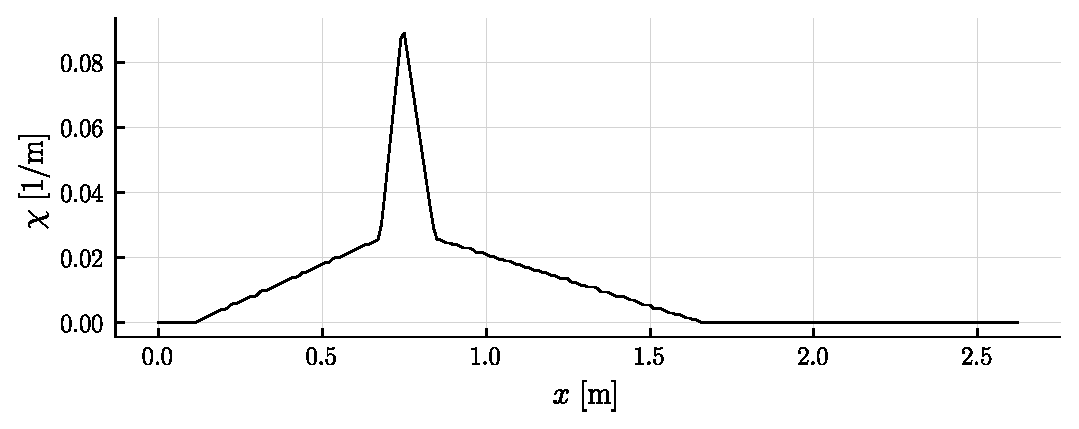
\includegraphics{index_files/mediabag/05_Versuchsnachrechnung_VM1_files/figure-pdf/fig-chi-max-a3v2-output-1.pdf}

}

\caption{\label{fig-chi-max-a3v2}Berechneter Krümmungsverlauf aus dem
Verdrehungsverlauf}

\end{figure}%

\newpage{}

\section{Vierpunktbiegeversuch}\label{vierpunktbiegeversuch}

Der Vierpunktbiegeversuch ist aus der Publikation
{[}\citeproc{ref-tue_einfluss_2019}{3}{]} entnommen. Es handelt sich um
einen Träger mit rechteckigem Querschnitt, gelagert als einfacher
Balken. Auffallend bei diesem Versuch ist die niedrig gehaltene
Schubbewehrung. Dazu sind in Längsrichtung Stäbe mit unterschiedlicher
Güte verlegt. Die Materialeigenschaften für den Bst 550 sind in
{[}\citeproc{ref-marienhutte_produktdatenblatt_b550bpdf_nodate}{4}{]}
ersichtlich.

\begin{figure}[H]

\centering{

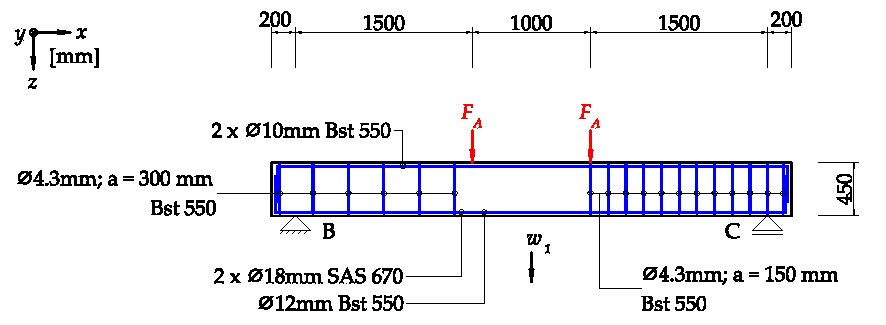
\includegraphics{index_files/mediabag/../imgs/versuchsskizze_14.pdf}

}

\caption{\label{fig-versuchsskizze-SV14}Bewehrungslayout des Versuchs
SV14, Zeichnung entnommen aus {[}\citeproc{ref-gitz_ansatze_2024}{1}{]}}

\end{figure}%

Die Abbildung~\ref{fig-versuchsskizze-SV14} zeigt die Lagerung des
Trägers, sowie die Stellen der Lasteinleitung. Zusätzlich ist das
Bewehrungslayout dargestellt. Der Querschnitt ist in der
Abbildung~\ref{fig-QS-SV14} gezeigt. Es ist lediglich die Längsbewehrung
dargestellt.

\begin{figure}[H]

\centering{

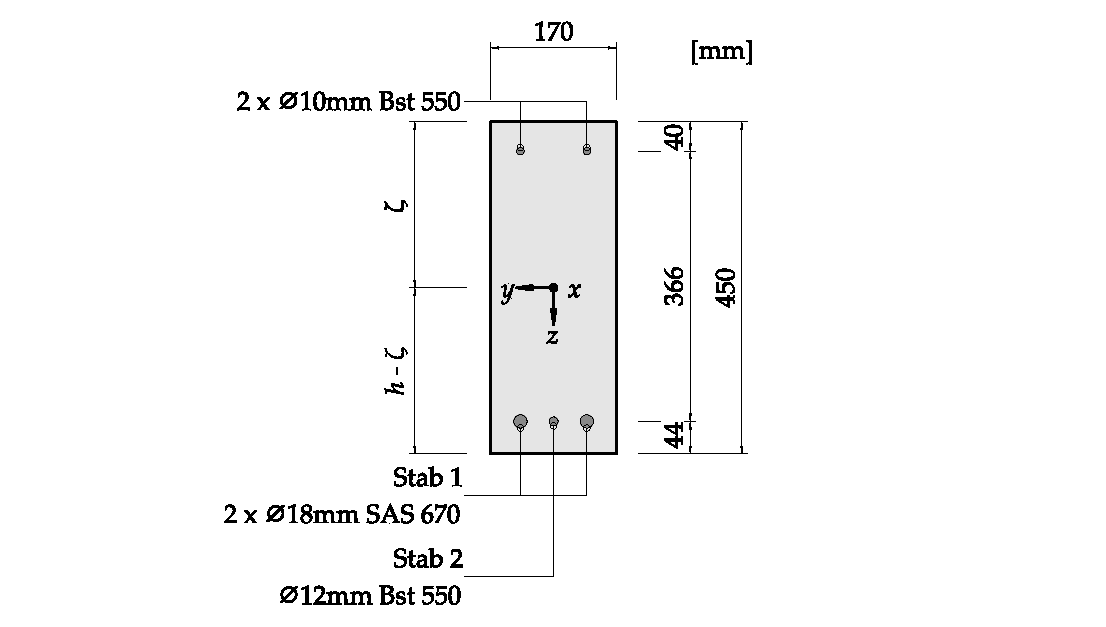
\includegraphics{index_files/mediabag/../imgs/QS_Versuch14.pdf}

}

\caption{\label{fig-QS-SV14}Querschnitt des Versuchs SV14, Zeichnung
entnommen aus {[}\citeproc{ref-gitz_ansatze_2024}{1}{]}}

\end{figure}%

Belastet wird der Träger an beiden Stellen \(F_A\) bis zum Versagen.
Aufgrund des unterschiedlichen Schubbewehrungsgehalts in beiden
Trägerhälften erfolgt zuerst ein Schubversagen in der schwächer
bewehrten Zone. Diese wird nachträglich verstärkt. Abschliessend wird
die Last gesteigert, bis ein Schubversagen in der stärker bewehrten Zone
eintritt. Die gemessenen Verformungen sind an der Stelle \(w_1\).

\subsection{Modellierung}\label{modellierung-1}

Das statische System ist in der Abbildung~\ref{fig-system-SV14} gezeigt.
Die Auflagerbreite wird vernachlässigt. Die Messungen der Durchbiegungen
zeigt, dass die Verformung bei \(F_A = 0\) ebenfalls null ist. Dies
führt zur Annahme, dass der Einfluss des Eigengewichts nicht gemessen
wurde. Somit wird dieses vernachlässigt.

\begin{figure}[H]

\centering{

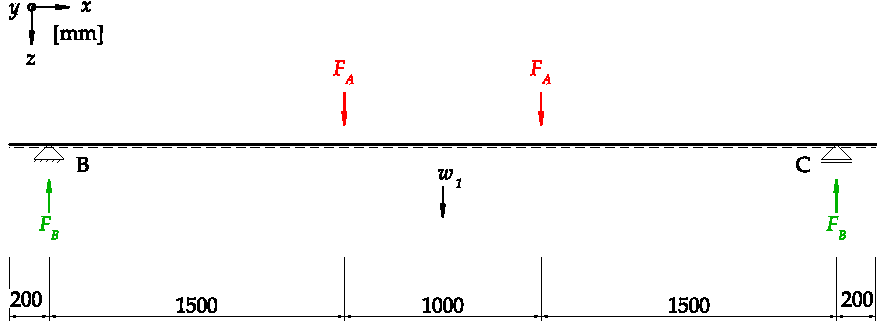
\includegraphics{index_files/mediabag/../imgs/statisches_system_14.pdf}

}

\caption{\label{fig-system-SV14}Statisches System des Versuchs SV14,
Zeichnung entnommen aus {[}\citeproc{ref-gitz_ansatze_2024}{1}{]}}

\end{figure}%

Auf die Darstellung der biegesteifen Elemente mit Endgelenken wird
verzichtet. Diese sind in einem Abstand von \(10\) mm entlang der
Stabachse verteilt.

$$
\begin{aligned}
l_{E} &= 10.0\ \mathrm{mm} \; \;\textrm{(Elementlänge des Biegesteifen Stabs)}
\end{aligned}
$$

Analog zum Dreipunktbiegeversuch wurde die Elementlänge mittels einer
Sensitivitätsanalyse emittelt. Eine feinere Stabunterteilung liefert
keine Verbesserung hinsichtlich der Präzision der Resultate.

\subsubsection{Biegeverformungen}\label{biegeverformungen-1}

Als Grundlage für die Drehfedercharakteristik gilt die
Momenten-Krümmungs-Beziehung. Für den Querschnitt des Versuchs SV14 gilt
die Beziehung gemäss Abbildung~\ref{fig-mchi_sv14}. Für detaillierte
Berechnungen ist die Vorarbeit {[}\citeproc{ref-gitz_ansatze_2024}{1}{]}
zu konsultieren. Die Beziehung wurde basierend auf bilinearen
Spannungs-Dehnungs-Beziehungen für den Betonstahl und linear-elastischen
ideal-plastischen Spannungs-Dehnungs-Beziehungen für den Beton mit
Berücksichtigung der Zugfestigkeit bestimmt.

\begin{figure}[H]

\centering{

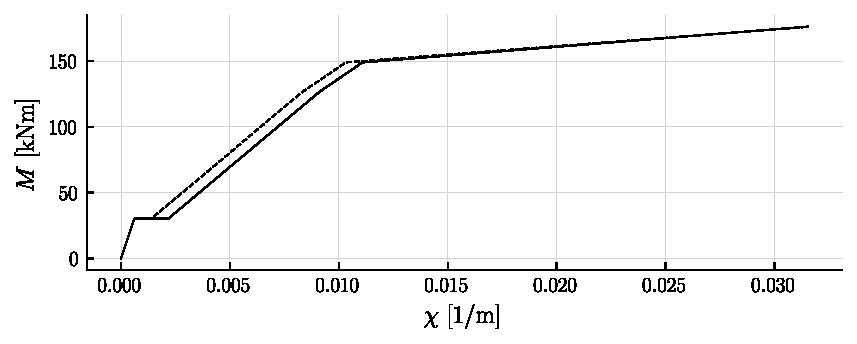
\includegraphics{index_files/mediabag/05_Versuchsnachrechnung_VM1_files/figure-pdf/fig-mchi_sv14-output-1.pdf}

}

\caption{\label{fig-mchi_sv14}Momenten-Krümmungs-Beziehung des
Vierpunktbiegeversuchs, übernommen aus
{[}\citeproc{ref-gitz_ansatze_2024}{1}{]}}

\end{figure}%

Die Momenten-Krümmungs-Beziehung beschreibt das Biegeverhalten des
Querschnitts für positive Biegung. Der Querschnitt ist deutlich steifer
vor dem Reissen. Nach dem Reissen des Querschnitts reduziert sich die
Biegesteifigkeit, dargestellt mit dem Bereich mit der Zugversteifung.
Die Zugversteifung wurde mittels dem Ansatz nach Marti, basierend auf
dem Zuggurtmodell bestimmt. In diesem Bereich ist ebenfalls ein Knick
erkennbar, dieser charaktisiert das Fliessen der schwächeren Bewehrung
im Zugbereich. Der grosse Steifigkeitsabfall resultiert durch das
Fliessen der starken Zugbewehrung.

\begin{figure}[H]

\centering{

\includegraphics{index_files/mediabag/05_Versuchsnachrechnung_VM1_files/figure-pdf/fig-mphi_sv14-output-1.pdf}

}

\caption{\label{fig-mphi_sv14}Momenten-Verdrehungs-Beziehung des
Vierpunktbiegeversuchs}

\end{figure}%

Die Momenten-Verdrehung-Beziehung ist in der
Abbildung~\ref{fig-mphi_sv14} dargestellt. Diese ist den Stabendgelenken
als Verdrehung in globaler \(Y\)-Richtung, gemäss dem Koordinatensystem
in der Abbildung~\ref{fig-system-SV14}, zu hinterlegen. Da die
Längsbewehrung nicht abgestuft ist, bzw. der Querschnitt für den
gesamten Stab gilt, ist diese Beziehung für sämtliche Elemente gültig.

\subsubsection{Versatzmass}\label{versatzmass}

Das Versatzmass berücksichtigt die Längszugkraft aus der Querkraft. Zur
Bestimmung des Versatzmass wird der Träger in Spannungsfelder
eingeteilt. Die Neigung der Spannungsfelder wird mittels der Traglast
bestimmt, welcher für den stärker schubbewehrten Bereich gilt. Es wird
ein Neigungswinkel \(\theta_{c3}\) gewählt um einen Querkraftwiderstand
zu erreichen, welcher der Traglast entspricht.

Anhand der Spannungsfeldeinteilung wird der Gurtkraftverlauf für den
unter- und den Obergurt bestimmt. Wird dem Zuggurt die Längszugkraft aus
dem Biegemoment subtrahiert, so resultiert das Versatzmass. Dies wird
folgend aufgezeigt. Zuerst sind die verwendeten Parameter aufgezeigt:

$$
\begin{aligned}
V_{exp_{sv14}} &= 105.0\ \mathrm{kN} \; 
 &z_{SV14} &= 359.0\ \mathrm{mm} \; 
 &\oslash_{sw_{SV14}} &= 4.3\ \mathrm{mm} \; 
\\[12pt]
 b_{w_{SV14}} &= 170.0\ \mathrm{mm} \; 
 &S_{sw_{SV14}} &= 150.0\ \mathrm{mm} \; 
 &f_{su_{SV14}} &= 715.0\ \frac{\mathrm{N}}{\mathrm{mm}^{2}} \; 
\\[12pt]
 \theta_{c3_{SV14}} &= 25.6\ \mathrm{°} \; 
 &F_{B} &= 105.0\ \mathrm{kN} \; 
 &F_{A} &= 105.0\ \mathrm{kN} \; 
\\[12pt]
\end{aligned}
$$

Mit der gewählten Neigung der Betondruckdiagonale resultiert der nötige
Querkraftwiderstand. Dazu wird zuerst die Querschnittsfläche der
Schubbewehrung bestimmt. Für den zweischenkligen Bügel folgt diese zu:

$$
\begin{aligned}
A_{sw_{SV14}} &= 2 \cdot \left( \frac{ \oslash_{sw_{SV14}} }{ 2 } \right) ^{ 2 } \cdot \pi \; 
\end{aligned}
$$

$$
\begin{aligned}
A_{sw_{SV14}} &= 29.0\ \mathrm{mm}^{2} \;
\end{aligned}
$$

Verschmiert über einen Meterstreifen resultiert:

$$
\begin{aligned}
a_{sw_{SV14}} &= \frac{ A_{sw_{SV14}} }{ S_{sw_{SV14}} } \; 
\end{aligned}
$$

$$
\begin{aligned}
a_{sw_{SV14}} &= 193.6\ \frac{\mathrm{mm}^{2}}{\mathrm{m}} \;
\end{aligned}
$$

Und abschliessend folgt der Querkraftwiderstand zu:

$$
\begin{aligned}
V_{Rd_{SV14}} &= a_{sw_{SV14}} \cdot z_{SV14} \cdot \frac{ f_{su_{SV14}} }{ \tan \left( \theta_{c3_{SV14}} \right) } \; 
\end{aligned}
$$

$$
\begin{aligned}
V_{Rd_{SV14}} &= 103.8\ \mathrm{kN} \;
\end{aligned}
$$

Der Querkraftwiderstand ist etwa gleich der Querkraft beim Erreichen der
Traglast. Die Spannungsfeldeinteilung ist in der
Abbildung~\ref{fig-spannungsfelder_sv14} gezeigt. Die Feldneigung ist
näherungsweise an die berechnete Neigung angepasst.

\begin{figure}[H]

\centering{

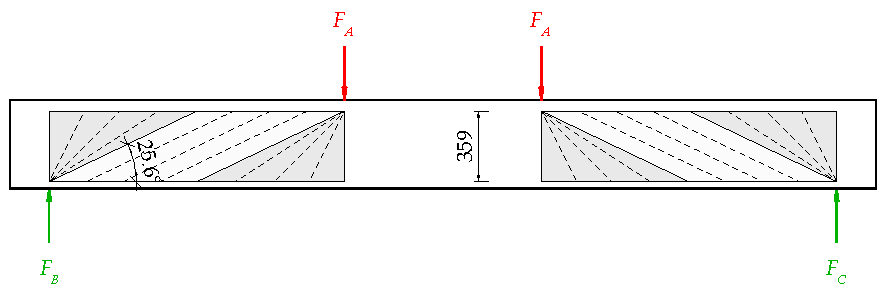
\includegraphics{index_files/mediabag/../imgs/SV14_spannungsfelder.pdf}

}

\caption{\label{fig-spannungsfelder_sv14}Einteilung in Spannungsfelder}

\end{figure}%

Wird nun Gleichgewicht an den entsprechenden Spannungsfeldern ausgeübt,
so lässt sich der Zug- und Druckkraftverlauf bestimmen. Für den
zentrierten Fächer beim Auflager gilt das Schnittkörperdiagramm in der
Abbildung~\ref{fig-skd_1_spannungsfelder_sv14}.

\begin{figure}[H]

\centering{

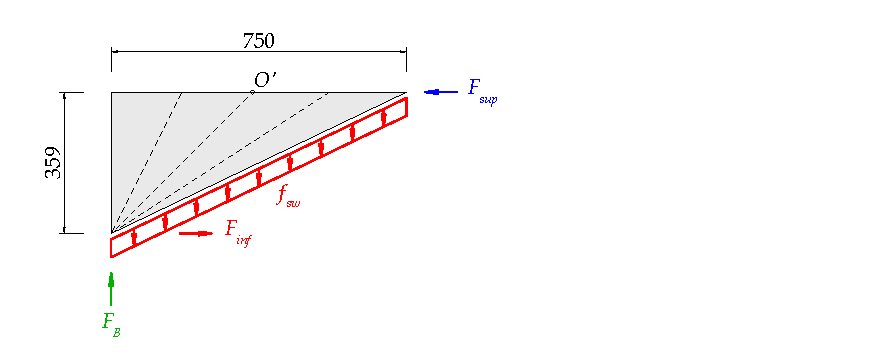
\includegraphics{index_files/mediabag/../imgs/SV14_skd_1.pdf}

}

\caption{\label{fig-skd_1_spannungsfelder_sv14}Schnittkörperdiagramm des
zentrierten Fächers}

\end{figure}%

Die Kraft im Untergurt lässt sich durch Momentengleichgewicht um den
Punkt \(O'\) bestimmen.

$$
\begin{aligned}
F_{inf_{1}} &= F_{B} \cdot \frac{ z_{SV14} }{ \tan \left( \theta_{c3_{SV14}} \right) } \cdot \frac{1} { 2 } \cdot \frac{1} { z_{SV14} } \; 
\end{aligned}
$$

$$
\begin{aligned}
F_{inf_{1}} &= 109.7\ \mathrm{kN} \; 
\end{aligned}
$$

Durch das Gleichgewicht der horizontalen Kräfte folgt die Obergurtkraft:

$$
\begin{aligned}
F_{sup_{1}} &= F_{inf_{1}} \; 
\end{aligned}
$$

$$
\begin{aligned}
F_{sup_{1}} &= 109.7\ \mathrm{kN} \; 
\end{aligned}
$$

Mittels Gleichgewicht der vertikalen Kräfte folgt die Kraft in der
Schubbewehrung:

$$
\begin{aligned}
f_{sw_{1}} &= \frac{ F_{B} }{ z_{SV14} } \cdot \frac{1} { \tan \left( \theta_{c3_{SV14}} \right) } \; 
\end{aligned}
$$

$$
\begin{aligned}
f_{sw_{1}} &= 611.0\ \frac{\mathrm{kN}}{\mathrm{m}} \;
\end{aligned}
$$

Am zentrierten Fächer schliesst das Parallelfeld an. Das entsprechende
Schnittkörperdiagramm zeigt die
Abbildung~\ref{fig-skd_2_spannungsfelder_sv14}.

\begin{figure}[H]

\centering{

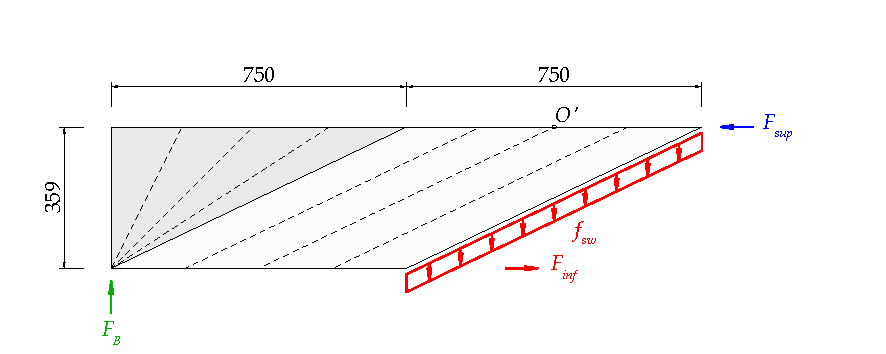
\includegraphics{index_files/mediabag/../imgs/SV14_skd_2.pdf}

}

\caption{\label{fig-skd_2_spannungsfelder_sv14}Schnittkörperdiagramm des
Parallelfelds}

\end{figure}%

Durch Gleichgewicht der Momente um den Punkt \(O'\) folgt wiederum die
Untergurtkraft:

$$
\begin{aligned}
F_{inf_{2}} &= F_{B} \cdot \frac{ 3 }{ 2 } \cdot \frac{ z_{SV14} }{ \tan \left( \theta_{c3_{SV14}} \right) } \cdot \frac{1} { z_{SV14} } \; 
\end{aligned}
$$

$$
\begin{aligned}
F_{inf_{2}} &= 329.0\ \mathrm{kN} \;
\end{aligned}
$$

Die Obergurtkraft folgt aus dem Gleichgewicht der horizontalen Kräfte:

$$
\begin{aligned}
F_{sup_{2}} &= F_{inf_{2}} \; 
\end{aligned}
$$

$$
\begin{aligned}
F_{sup_{2}} &= 329.0\ \mathrm{kN} \; 
\end{aligned}
$$

Abschliessend folgt die Kraft in der Schubbewehrung zu:

$$
\begin{aligned}
f_{sw_{2}} &= \frac{ F_{B} }{ z_{SV14} } \cdot \frac{1} { \tan \left( \theta_{c3_{SV14}} \right) } \; 
\end{aligned}
$$

$$
\begin{aligned}
f_{sw_{2}} &= 611.0\ \frac{\mathrm{kN}}{\mathrm{m}} \;
\end{aligned}
$$

Das Schnittkörperdiagramm bei der Krafteinleitung ist in der
Abbildung~\ref{fig-skd_3_spannungsfelder_sv14} gezeigt.

\begin{figure}[H]

\centering{

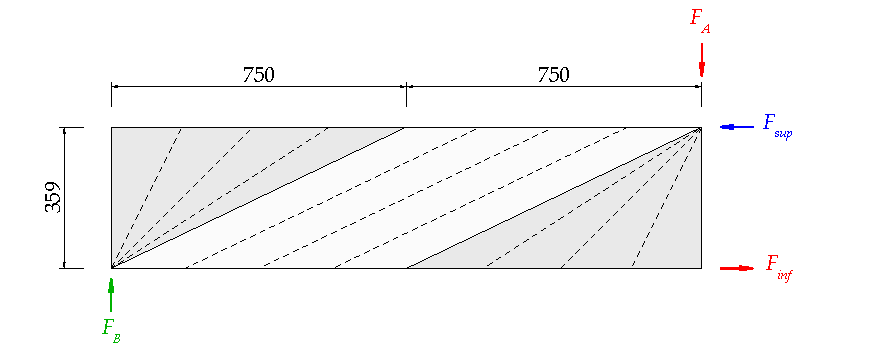
\includegraphics{index_files/mediabag/../imgs/SV14_skd_3.pdf}

}

\caption{\label{fig-skd_3_spannungsfelder_sv14}Schnittkörperdiagramm des
zentrierten Fächers 2}

\end{figure}%

Die Untergurtkraft folgt zu:

$$
\begin{aligned}
F_{inf_{3}} &= F_{B} \cdot 2 \cdot \frac{ z_{SV14} }{ \tan \left( \theta_{c3_{SV14}} \right) } \cdot \frac{1} { z_{SV14} } \; 
\end{aligned}
$$

$$
\begin{aligned}
F_{inf_{3}} &= 438.7\ \mathrm{kN} \;
\end{aligned}
$$

Die Obergurtkraft entspricht dabei:

$$
\begin{aligned}
F_{sup_{3}} &= F_{inf_{3}} \; 
\end{aligned}
$$

$$
\begin{aligned}
F_{sup_{3}} &= 438.7\ \mathrm{kN} \;
\end{aligned}
$$

Damit ist abschliessend der Gurtkraftverlauf definiert. Dargestellt ist
dieser in Abbildung~\ref{fig-gurtkraft_sv14}. Ebenfalls aufgezeigt ist
der Anteil im Untergurt aus dem Biegemoment. Die Differenz zwischen der
gesamten Untergurtkraft und dem Anteil aus dem Biegemoment führt zum
Versatzmass.

\begin{figure}[H]

\centering{

\includegraphics{index_files/mediabag/05_Versuchsnachrechnung_VM1_files/figure-pdf/fig-gurtkraft_sv14-output-1.pdf}

}

\caption{\label{fig-gurtkraft_sv14}Gurtkraftverläufe bestimmt anhand der
Spannungsfelder in Abbildung~\ref{fig-spannungsfelder_sv14}. Dargestellt
ist der gesamte Gurtkraftverlauf, sowie der Anteil aus dem Biegemoment}

\end{figure}%

Wird der Anteil des Biegemoments am Gurtkraftverlauf subtrahiert und mit
dem Hebelarm der inneren Kräfte multipliziert, so resultiert das
Versatzmoment.

\[
\Delta_F = F_{inf} - F_M
\] \[
\Delta_M = \Delta_F \cdot z
\]

Das Versatzmoment ist in der Abbildung~\ref{fig-versatzmoment_sv14}
entlang der Stabachse aufgezeigt. Dieses wird dem Modell auf Seiten der
Einwirkung hinterlegt. Es wird ein Lastfall definiert, welcher zu dem
Biegemomentenverlauf gemäss dem Versatzmass führt.

\begin{figure}[H]

\centering{

\includegraphics{index_files/mediabag/05_Versuchsnachrechnung_VM1_files/figure-pdf/fig-versatzmoment_sv14-output-1.pdf}

}

\caption{\label{fig-versatzmoment_sv14}Versatzmoment dargestellt entlang
der Stabachse}

\end{figure}%

\subsubsection{Schubverformungen}\label{schubverformungen-1}

Die Schubverformungen werden im Modell mittels einer
Wegfedercharakteristik in globaler \(Z\)-Richtung, gemäss dem
Koordinatensystem in der Abbildung~\ref{fig-system-SV14},
berücksichtigt. Die Wegfedercharakteristik basiert auf der
Spannungsfeldmodellierung gemäss der
Abbildung~\ref{fig-spannungsfelder_sv14}. Es wird vorausgesetzt, dass
sämtliche Verformung aus der Schubbewehrung erfolgt, ein Mitwirken des
Betons wird vernachlässigt. Die Einteilung in Spannungsfelder ermöglicht
die Bestimmung der mitwirkenden Schubbewehrung beim Versagen des
Querschnitts. Die Neigung des Feldes ist so gewählt damit der
Querkraftwiderstand der Schubbewehrung der Traglast des Systems
entspricht.

\begin{figure}[H]

\centering{

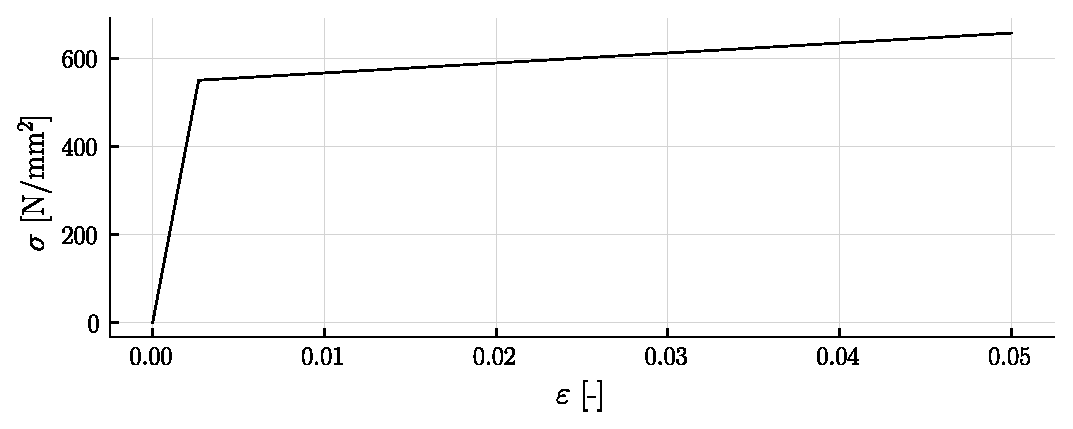
\includegraphics{index_files/mediabag/05_Versuchsnachrechnung_VM1_files/figure-pdf/fig-sigma-epsilon-sv14-output-1.pdf}

}

\caption{\label{fig-sigma-epsilon-sv14}Spannungs-Dehnungs-Beziehung der
Schubbewehrung, übernommen aus
{[}\citeproc{ref-gitz_ansatze_2024}{1}{]}}

\end{figure}%

Wird das Spannungs-Dehnungs-Verhalten gemäss der
Abbildung~\ref{fig-sigma-epsilon-sv14} berücksichtigt. So resultiert mit
der Querschnittsfläche der Schubbewehrung pro Spannungsfeld die
entsprechende Kraftkomponente der Wegfedercharakteristik. Die
Verformungskomponente entspricht der Dehnung multipliziert mit dem
Hebelarm der inneren Kräfte. Dies führt zum Kraft-Verformungs-Verhalten
für ein Spannungsfeld. Um die Wegfedercharakteristik eines einzelnen
Stabendgelenks zu erhalten, ist die Verformung um die Anzahl an
Stabelementen im Spannungsfeld zu reduzieren.

Die verwendeten Parameter sind bereits bei der Bestimmung des
Versatzmass aufgezeigt, lediglich der Elastizitätsmodul findet noch
Einfluss in die Berechnung.

$$
\begin{aligned}
E_{sw_{SV14}} &= 205000.0\ \frac{\mathrm{N}}{\mathrm{mm}^{2}} \;
\end{aligned}
$$

Der Reduktionsfaktor zur Erhöhung der Steifigkeit des Stabendgelenks
folgt zu:

$$
\begin{aligned}
\gamma_{E_{SV14}} &= z_{SV14} \cdot \frac{ 1 }{ \tan \left( \theta_{c3_{SV14}} \right) } \cdot \frac{1} { l_{E} } \; 
\end{aligned}
$$

$$
\begin{aligned}
\gamma_{E_{SV14}} &= 75\ \;
\end{aligned}
$$

Die Abbildung~\ref{fig-wegfeder-schub-sv14} zeigt das
Kraft-Verformungs-Verhalten für die Gelenke des Stabmodells in
vertikaler Richtung. Das Verhalten ist analog dem des biliniearen
Spannungs-Dehnungs-Diagramms.

\begin{figure}[H]

\centering{

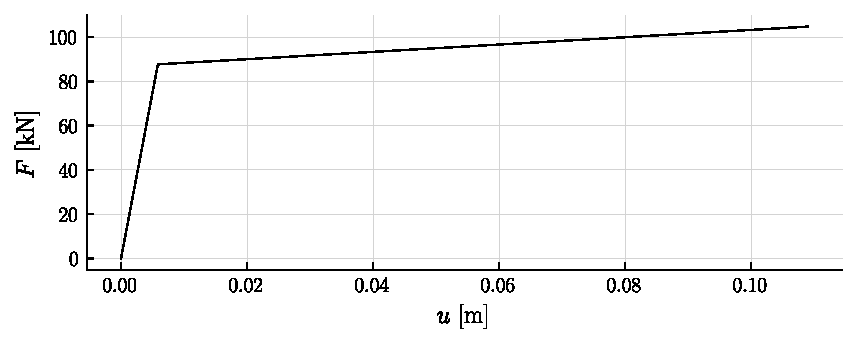
\includegraphics{index_files/mediabag/05_Versuchsnachrechnung_VM1_files/figure-pdf/fig-wegfeder-schub-sv14-output-1.pdf}

}

\caption{\label{fig-wegfeder-schub-sv14}Berechnete
Wegfedercharakteristik des Schubgelenks vom Versuch SV14}

\end{figure}%

\subsection{Ergebnisse}\label{ergebnisse-1}

Mit den bestimmten Federcharakteristiken kann die Biegelinie des Systems
ermittelt werden unter Berücksichtigung der Schub- und Biegeverformungen
auf nicht-linearen Grundlagen. Die Abbildung~\ref{fig-l-w-sv14} zeigt
das Last-Verformungs-Diagramm des Systems am Punkt \(w_1\). Der
Verformungsverlauf zeigt Abweichungen zu den gemessenen Resultate.

\begin{figure}[H]

\centering{

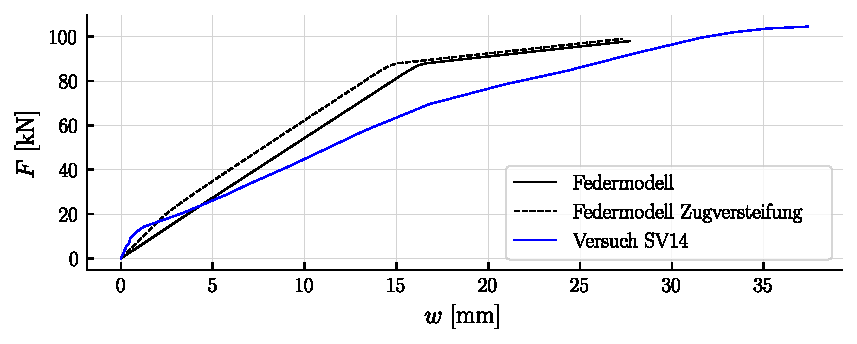
\includegraphics{index_files/mediabag/05_Versuchsnachrechnung_VM1_files/figure-pdf/fig-l-w-sv14-output-1.pdf}

}

\caption{\label{fig-l-w-sv14}Last-Verformungs-Verlauf am Punkt \(w_1\),
für das Federmodell und den Versuch}

\end{figure}%

Bis zum Erreichen des ersten Knicks im Verlauf des Federmodells ist das
Modell etwas zu steif. Trotzdem ist dies akzeptabel. Der Knick
resultiert aus dem Fliessen der Schubbewehrung. Bei den
Versuchsresultaten ist bei gleicher Verformung ebenfalls ein Knick zu
erkennen. Jedoch lässt sich daraus schliessen, dass die Schubbewehrung
bei einem zu hohen Lastniveau beginnt zu fliessen, sowie ist das
verfestigende Verhalten nicht gleich mit dem Versuchsverhalten.
Möglicherweise müssten die Fliessspannung und die Zugfestigkeit der
Schubbewehrung angepasst werden, bzw. nicht aus genormten
Produktedokumentation entnommen werden. Sondern aus effektiven
Materialproben.

\begin{figure}[H]

\centering{

\includegraphics{index_files/mediabag/05_Versuchsnachrechnung_VM1_files/figure-pdf/fig-phi-max-sv14-output-1.pdf}

}

\caption{\label{fig-phi-max-sv14}Verdrehungsverlauf aus dem Federmodell
für die Höchstlast des Versuchs SV14}

\end{figure}%

Der Krümmungsverlauf gibt Aufschluss über den Fliessbereich der
Bewehrung, bzw. über den Steifigkeitenverlauf entlang der Stabachse.

\begin{figure}[H]

\centering{

\includegraphics{index_files/mediabag/05_Versuchsnachrechnung_VM1_files/figure-pdf/fig-chi-max-sv14-output-1.pdf}

}

\caption{\label{fig-chi-max-sv14}Berechneter Krümmungsverlauf aus dem
Verdrehungsverlauf für den Versuch SV14}

\end{figure}%

\section{Schlussfolgerung}\label{schlussfolgerung}

Das Kapitel der Modellverifizierung zeigt auf, dass mittels dem Modell
die Versuchsresultate zufriedenstellend nachgerechnet werden können. Das
Modell ermöglicht die Berücksichtigung des Versatzmass, sowie
Verformungen basierend auf nicht-linearen Biege- und Schubbeziehung.

\bookmarksetup{startatroot}

\chapter{Vorgespannter Träger}\label{vorgespannter-truxe4ger}

Nachdem das Kapitel~\ref{sec-verifizierung} die Anwendbarkeit des
Modells bestätigt hat, wird in diesem Kapitel ein Versuch eines
vorgespannten Trägers mittels dem Federmodell nachgerechnet. Es wird die
Bestimmung der Momenten-Krümmungs-Beziehung aufgezeigt. Auf das
Versatzmass und auf die Schubverformungen wird nicht eingegangen.
Abschliessend werden die Versuchsresultate mit den berechneten Grössen
verglichen und kommentiert.

\section{Versuchsbeschrieb}\label{versuchsbeschrieb}

Der vorgespannte Träger T6 ist im Versuchsbericht
{[}\citeproc{ref-sigrist_versuche_1993}{5}{]} aufgezeigt. Es handelt
sich um einen einfachen Balken mit einer Auskragung. Die Geometrie des
Versuchs in Längsrichtung ist in Abbildung~\ref{fig-geometrie_t6}
gezeigt.

\begin{figure}[H]

\centering{

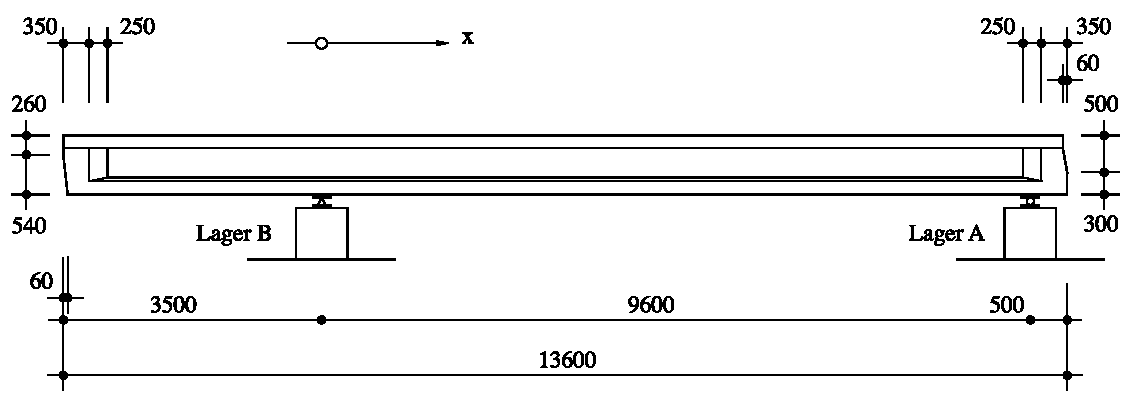
\includegraphics{index_files/mediabag/../imgs/T6_geometrie_laengs.pdf}

}

\caption{\label{fig-geometrie_t6}Geometrie des Versuchsträgers T6,
entnommen aus {[}\citeproc{ref-sigrist_versuche_1993}{5}{]}}

\end{figure}%

Der dazugehörige Querschnitt ist in Abbildung~\ref{fig-geometrie_qs_t6}
gezeigt.

\begin{figure}[H]

\centering{

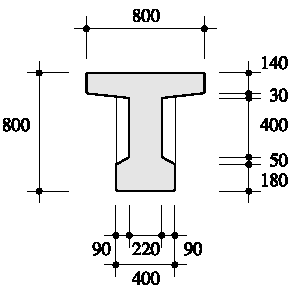
\includegraphics{index_files/mediabag/../imgs/T6_geometrie_qs.pdf}

}

\caption{\label{fig-geometrie_qs_t6}Geometrie des Querschnitts des
Versuchsträgers T6, entnommen aus
{[}\citeproc{ref-sigrist_versuche_1993}{5}{]}}

\end{figure}%

Die Lastsituation zeigt die Abbildung~\ref{fig-last_t6}. Am Ende des
Kragarms greift eine Einzellast \(P\) an. Mit \(Q\) wird eine
Streckenlast simuliert. Der Träger ist an den Punkten \(A\) und \(B\)
gelenkig gelagert. Zusätzlich ist der Träger beim Auflager \(B\)
horizontal gehalten.

\begin{figure}[H]

\centering{

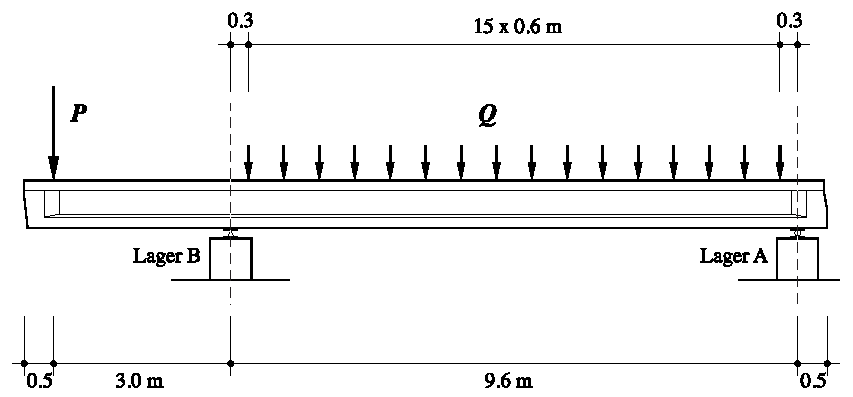
\includegraphics{index_files/mediabag/../imgs/T6_last_laengs.pdf}

}

\caption{\label{fig-last_t6}Lagerung und Laststellung des
Versuchsträgers T6, entnommen aus
{[}\citeproc{ref-sigrist_versuche_1993}{5}{]}}

\end{figure}%

Die verlegte schlaffe Bewehrung ist in der
Abbildung~\ref{fig-bewehrung_laengs_t6} gezeigt. Diese ist an mehreren
Punkten abgestuft. Die Stosslänge beträgt jeweils \(60\) cm. Mit
Grossbuchstaben \(A\) bis \(I\) sind die Bewehrungslagen in
längsrichtung beschrieben. Die Schubbügel sind mit den Kleinbuchstaben
\(i\) bis \(iii\) bezeichnet.

\begin{figure}[H]

\centering{

\includegraphics{index_files/mediabag/../imgs/T6_bewehrung_laengs.pdf}

}

\caption{\label{fig-bewehrung_laengs_t6}Bewehrungslayout in
Längsrichtung des Versuchsträgers T6, entnommen aus
{[}\citeproc{ref-sigrist_versuche_1993}{5}{]}}

\end{figure}%

Das Bewehrungslayout im Querschnitt zeigt die
Abbildung~\ref{fig-bewehrung_qs_t6}. Die Bewehrungsüberdeckung beträgt
in allen Richtungen \(20\) mm.

\begin{figure}[H]

\centering{

\includegraphics{index_files/mediabag/../imgs/T6_bewehrung_qs.pdf}

}

\caption{\label{fig-bewehrung_qs_t6}Bewehrungslayout im Querschnitt des
Versuchsträgers T6, entnommen aus
{[}\citeproc{ref-sigrist_versuche_1993}{5}{]}}

\end{figure}%

Die Führung der Vorspannung ist in der
Abbildung~\ref{fig-vorspannung_t6} gezeigt. Das Kabel konnte im Mittel
bis auf \(730\) kN vorgespannt werden. Das Spannkabel besteht aus 4
Litzen mit Durchmesser \(0.6''\). Eingelegt sind diese in ein
Stahlhüllrohr, welches nachträglich ausinjiziert wurde.

\begin{figure}[H]

\centering{

\includegraphics{index_files/mediabag/../imgs/T6_vorspannung_laengs.pdf}

}

\caption{\label{fig-vorspannung_t6}Vorspannungslayout des
Versuchsträgers T6. Horizontaler Abstand {[}m{]} und vertikale Position
{[}mm{]}, gemessen von der Unterkante des Trägers, entnommen aus
{[}\citeproc{ref-sigrist_versuche_1993}{5}{]}}

\end{figure}%

\subsection{Parameter}\label{parameter}

In diesem Abschnitt werden die allgemein verwendeten Parameter
aufgelistet. Gegliedert nach den einzelnen Aspekten des Versuchs.

\subsubsection{Vorspannung}\label{vorspannung}

Der folgende Abschnitt charakterisiert die Vorspannung. Aufgezeigt ist
die mittlere initiale Vorspannkraft, die Fliessgrenze der Litzen, sowie
deren Zugfestigkeit und entprechende Bruchdehnung. Ebenfalls dargestellt
ist der Elasitzitätsmodul, die Querschnittsfläche des Spannglieds und
der angewendete Verlustfaktor.

\begin{figure}[H]

\centering{

\includegraphics{index_files/mediabag/../imgs/t6_spannstahl.pdf}

}

\caption{\label{fig-sigma_eps_spannstahl}Spannungs-Dehnungs-Diagramm
mittels Zugproben ermittelt für den Spannstahl}

\end{figure}%

$$
\begin{aligned}
f_{py} &= 1706.0\ \frac{\mathrm{N}}{\mathrm{mm}^{2}} \; 
 &f_{pt} &= 1855.0\ \frac{\mathrm{N}}{\mathrm{mm}^{2}} \; 
 &V_{om} &= 730.0\ \mathrm{kN} \; 
\\[10pt]
 A_{p} &= 596.0\ \mathrm{mm}^{2} \; 
 &E_{p} &= 190000.0\ \frac{\mathrm{N}}{\mathrm{mm}^{2}} \; 
 &\varepsilon_{pu} &= 1.5\ \mathrm{\%} \; 
\\[10pt]
 \eta &= 0.9 \; \;\textrm{(Verlustfaktor)}
\end{aligned}
$$

Der Verlustfaktor wird ohne Berücksichtigung von Langzeiteffekten auf
90\% geschätzt. Daras resultiert die Vorspannkraft zu:

$$
\begin{aligned}
P_{\infty} &= \eta \cdot V_{om} \; 
\end{aligned}
$$

$$
\begin{aligned}
P_{\infty} &= 657.0\ \mathrm{kN} \;
\end{aligned}
$$

Die Spannung im Spannglied aufgrund der Vorspannung defniert sich zu:

$$
\begin{aligned}
\sigma_{P_{\infty}} &= \frac{ P_{\infty} }{ A_{p} } \; 
\end{aligned}
$$

$$
\begin{aligned}
\sigma_{P_{\infty}} &= 1102.3\ \frac{\mathrm{N}}{\mathrm{mm}^{2}} \;
\end{aligned}
$$

Wird nun das Spannungs-Dehnungs-Verhalten des Spannstahls betrachtet, so
ist ersichtlich, dass durch die Vorspannung die Spannlitzen noch nicht
ausgeschöpft sind. Dargestellt ist dies in der
Abbildung~\ref{fig-ausnutzung_sigma_p}. Unter dieser Voraussetzung
beteiligt sich das Vorspannkabel ebenfalls am Abtrag der Biegemomente,
bzw. fliesst in die Momenten-Krümmungs-Beziehung mit ein.

\begin{figure}[H]

\centering{

\includegraphics{index_files/mediabag/06_Vorspannversuch_files/figure-pdf/fig-ausnutzung_sigma_p-output-1.pdf}

}

\caption{\label{fig-ausnutzung_sigma_p}Spannungs-Dehnungs-Beziehung der
Spannlitzen mit ergänzter Ausnutzung durch die Vorspannung}

\end{figure}%

\subsubsection{Beton}\label{beton}

Die Parameter sind Mittelwerte aus Betonwürfel- und Betonzylinderproben.
Entnommen aus dem Versuchsbericht
{[}\citeproc{ref-sigrist_versuche_1993}{5}{]}. In der
Abbildung~\ref{fig-sigma_eps_beton} ist das Spannungs-Dehnungs-Verhalten
der Betonproben aufgezeigt.

\begin{figure}[H]

\centering{

\includegraphics{index_files/mediabag/../imgs/t6_beton.pdf}

}

\caption{\label{fig-sigma_eps_beton}Spannungs-Dehnungs-Diagramm für den
Beton, dargestellt sind diese für die Versuchskörper \(T_1\) bis
\(T_6\)}

\end{figure}%

Dabei beschreibt \(f_c\) die maximale Druckfestigkeit.

$$
\begin{aligned}
f_{c} &= 52.10\ \frac{\mathrm{N}}{\mathrm{mm}^{2}} \; 
 &f_{cts} &= 4.30\ \frac{\mathrm{N}}{\mathrm{mm}^{2}} \; 
 &E_{c} &= 50200.00\ \frac{\mathrm{N}}{\mathrm{mm}^{2}} \; 
\\[10pt]
 \rho_{c} &= 2409.00\ \frac{\mathrm{kg}}{\mathrm{m}^{3}} \; 
 &\varepsilon_{cu} &= 0.35\ \mathrm{\%} \;
\end{aligned}
$$

\subsubsection{Betonstahl}\label{betonstahl}

Die dargestellten Parameter sind Mittelwerte aus den durchgeführten
Zugproben. Diese sind ebenfalls aus dem Versuchsbericht
{[}\citeproc{ref-sigrist_versuche_1993}{5}{]} entnommen.

\begin{figure}[H]

\centering{

\includegraphics{index_files/mediabag/../imgs/t6_betonstahl.pdf}

}

\caption{\label{fig-sigma_eps_betonstahl}Spannungs-Dehnungs-Diagramm und
Kraft-Verformungs-Diagramm mittels Zugproben ermittelt für den
Betonstahl}

\end{figure}%

Die Abbildung~\ref{fig-sigma_eps_betonstahl} zeigt das
Spannungs-Dehnungs-Verhalten, sowie das Kraft-Verformungs-Verhalten der
Probe eines Durchmesser \(16\) mm Stabs. Im Spannungs-Dehnungs-Diagramm
ist lediglich das Fliessplateau dargestellt.

$$
\begin{aligned}
f_{sy} &= 500.0\ \mathrm{MPa} \; 
 &f_{st} &= 630.0\ \mathrm{MPa} \; 
 &\varepsilon_{su} &= 12.7\ \mathrm{\%} \; 
\\[10pt]
 E_{s} &= 205000.0\ \frac{\mathrm{N}}{\mathrm{mm}^{2}} \;
\end{aligned}
$$

\subsubsection{Geometrie}\label{geometrie}

Die Parameter der Geometrie des Querschnitts beziehen sich auf die
Abbildung~\ref{fig-geometrie_qs_t6}. Der Schwerpunkt \(S_z\) des
Querschnitts ist von der Unterkante aus gemessen.

$$
\begin{aligned}
h_{1} &= 180.0\ \mathrm{mm} \; 
 &h_{2} &= 50.0\ \mathrm{mm} \; 
 &h_{3} &= 400.0\ \mathrm{mm} \; 
\\[10pt]
 h_{4} &= 30.0\ \mathrm{mm} \; 
 &h_{5} &= 140.0\ \mathrm{mm} \; 
 &h &= 800.0\ \mathrm{mm} \; 
\\[10pt]
 b_{1_{inf}} &= 90.0\ \mathrm{mm} \; 
 &b_{2_{inf}} &= 220.0\ \mathrm{mm} \; 
 &b_{3_{inf}} &= 90.0\ \mathrm{mm} \; 
\\[10pt]
 b_{inf} &= 400.0\ \mathrm{mm} \; 
 &b_{sup} &= 800.0\ \mathrm{mm} \; 
 &S_{z} &= \mathtt{\text{464.00 mm}} \; 
\\[10pt]
 L &= 13600.0\ \mathrm{mm} \;
\end{aligned}
$$

\subsection{Versuchsergebnisse}\label{versuchsergebnisse}

Der Versuchsbeschrieb wird mit den gemessenen Resultate abgeschlossen.
Die Abbildung~\ref{fig-durchbiegung_laengs_t6} zeigt den
Verformungsverlauf für den gesamten Träger für die entsprechenden
Laststufen.

\begin{figure}[H]

\centering{

\includegraphics{index_files/mediabag/../imgs/T6_durchbiegung_laengs.pdf}

}

\caption{\label{fig-durchbiegung_laengs_t6}Verformungsverlauf des
Versuchsträgers T6, entnommen aus
{[}\citeproc{ref-sigrist_versuche_1993}{5}{]}}

\end{figure}%

Die Abbildung~\ref{fig-durchbiegung_t6} zeigt oben links das
Kraft-Verformungs-Diagramm für die Einzellast \(P\) mit der gemessenen
Verformung \(w_{10}\) an der Stelle \(10\), gemäss der
Abbildung~\ref{fig-messstellen_t6}. Oben rechts ist das
Kraft-Verformungs-Diagramm für die simulierte Streckenlast \(Q\) und die
Verformung \(w_18\) aufgezeigt.

\begin{figure}[H]

\centering{

\includegraphics{index_files/mediabag/../imgs/t6_messstellen.pdf}

}

\caption{\label{fig-messstellen_t6}Messstellen des Trägers T6, entnommen
aus {[}\citeproc{ref-sigrist_versuche_1993}{5}{]}}

\end{figure}%

Das Diagramm unten links gibt Aufschluss über den Belastungshergang.
Zunächst wird die Einzelllast \(P\) gesteigert bis ca. \(480\) kN. Ab
dieser Stufe wurde die Einzellast konstant gehalten, die Streckenlast
\(Q\) wurde abschliessend erhöht, bis der Träger versagte. Das Versagen
geschah schlagartig, durch das Versagen der Vorspannlitzen.

\begin{figure}[H]

\centering{

\includegraphics{index_files/mediabag/../imgs/T6_durchbiegungen.pdf}

}

\caption{\label{fig-durchbiegung_t6}Last-Verformungs-Verhalten des
Versuchsträgers T6, entnommen aus
{[}\citeproc{ref-sigrist_versuche_1993}{5}{]}}

\end{figure}%

\section{Modellierung}\label{modellierung-2}

Der vorangegangen Abschnitt beschreibt den Versuch ausführlich. In
diesem Abschnitt wird auf die Modellierung des Problems eingegangen. Der
Versuch wird mittels dem Federmodell modelliert. Den Federn wird eine
entsprechende Drehfedercharakteristik hinterlegt. Als Grundlage dient
das statische System in der Abbildung~\ref{fig-system_t6}.

\begin{figure}[H]

\centering{

\includegraphics{index_files/mediabag/../imgs/T6_system.pdf}

}

\caption{\label{fig-system_t6}Statisches System des Versuchs \(T_6\)}

\end{figure}%

Die Auflagerbreiten sind vernachlässigt. Auf die Darstellung der Federn
wird verzichtet. Diese sind in einem Abstand von \(l_E\) angeordnet.

$$
\begin{aligned}
l_{E} &= 10.0\ \mathrm{cm} \; \;\textrm{(Elementlänge des biegesteifen Stabs)}
\end{aligned}
$$

Die Elementlänge wird im Vergleich mit den Versuchen aus dem Kapitel
Kapitel~\ref{sec-verifizierung} deutlich grober gewählt. Dies ist auf
die aufwändige Bestimmung der Momenten-Krümmungs-Beziehung
zurückzuführen.

\subsection{Lastfälle}\label{lastfuxe4lle}

Die unterschiedliche Belastungsgeschwindigkeit liefert eine gewisse
Komplexität bei der Modellierung. Sowie wird die Vorspannung als
Einwirkung interpretiert. Abschliessend ist aufgrund der Vorspannung das
Eigengewicht zu berücksichtigen, da dies den positiv gerichteten
Umlenkkräften entgegen wirkt. Es wird zwischen den Lastfällen
Eigengewicht, Vorspannung und zweier Versuchslasten unterschieden.

\subsubsection{Eigengewicht}\label{eigengewicht}

Das Eigengewicht wird als Streckenlast auf dem gesamten statischen
System angeordnet. Ermittelt aus der Betonquerschnittsfläche und
entsprechender Dichte.

\begin{figure}[H]

\centering{

\includegraphics{index_files/mediabag/../imgs/T6_eigengewicht_lf.pdf}

}

\caption{\label{fig-t6_lastfall_eg}Statisches System mit Streckenlast
durch Eigengewicht}

\end{figure}%

$$
\begin{aligned}
A_{c} &= 285200.0\ \mathrm{mm}^{2} \;
\end{aligned}
$$

$$
\begin{aligned}
q_{c} &= A_{c} \cdot \rho_{c} \cdot 10 \cdot \frac{ m }{ \left( s \right) ^{ 2 } } \; 
\end{aligned}
$$

$$
\begin{aligned}
q_{c} &= 6.9\ \frac{\mathrm{kN}}{\mathrm{m}} \;
\end{aligned}
$$

\subsubsection{Versuch}\label{versuch}

\begin{figure}[H]

\centering{

\includegraphics{index_files/mediabag/../imgs/T6_versuch_lf.pdf}

}

\caption{\label{fig-t6_lastfall_versuch}Statisches System mit
Versuchslasten}

\end{figure}%

Gemäss dem Versuchsbeschrieb lässt sich der Träger bis zu den folgenden
maximalen Lasten belasten:

$$
\begin{aligned}
Q_{max} &= 1638.0\ \mathrm{kN} \; 
 &P_{max} &= 512.0\ \mathrm{kN} \; 
 &L_{q} &= 9.0\ \mathrm{m} \; 
\\[10pt]
\end{aligned}
$$

Die mit \(Q\) simulierte Streckenlast wird als effektive Streckenlast
modelliert. Dies führt zu folgender Grösse:

$$
\begin{aligned}
q_{Q_{max}} &= \frac{ Q_{max} }{ L_{q} }  = \frac{ 1638.0\ \mathrm{kN} }{ 9.0\ \mathrm{m} } &= 182.0\ \frac{\mathrm{kN}}{\mathrm{m}}  
\end{aligned}
$$

Im Stabstatik-Modell werden zwei Lastfälle definiert zum Abbilden der
Versuchslast. Zum einen wird die maximale Einzellast \(P_{LS8}\) und die
entsprechende Streckenlast \(q_{LS8}\) gemäss der Laststufe 8,
aufgezeigt in der Abbildung~\ref{fig-durchbiegung_t6}, modelliert.
Dieser Lastfall wird in Laststufen unterteilt bei der Berechnung und
liefert so Resultate für sämtliche Laststufen unterhalb der Laststufe 8.

$$
\begin{aligned}
P_{LS8} &= 471.0\ \mathrm{kN} \; 
 &q_{LS8} &= 85.0\ \frac{\mathrm{kN}}{\mathrm{m}} \; 
 &Q_{LS8} &= 765.0\ \mathrm{kN} \; 
\\[10pt]
\end{aligned}
$$

Der zweite Lastfall beinhaltet die konstante Einzellast \(P_{LS12}\),
sowie die Streckenlast \(q_{Q_{LS12}} - q_{LS8}\). In diesem Lastfall
wird lediglich die Streckenlast in Laststufen unterteilt.

$$
\begin{aligned}
P_{LS12} &= 471.0\ \mathrm{kN} \; 
 &q_{LS12} &= 163.0\ \frac{\mathrm{kN}}{\mathrm{m}} \; 
 &Q_{LS12} &= 1467.0\ \mathrm{kN} \; 
\\[10pt]
\end{aligned}
$$

Das Modell konvergiert bei der Applikation der Traglast nicht mehr. Aus
diesem Grund wird die maximale Streckenlast reduziert.

\subsubsection{Vorspannung}\label{vorspannung-1}

Unabhängig von der Versuchslast gilt es den Einfluss der Vorspannung auf
das System zu modellieren. Dazu wird die Vorspannung als Anker - Umlenk
- und Reibungskräfte (AUR) interpretiert. Grundlagen dazu sind in
{[}\citeproc{ref-thoma_vorspannung_2020}{6}{]} aufgezeigt. Die
Interpretation nach AUR führt zu Umlenkkräften im parabolischen Bereich
der Vorspannung, sowie zu Normal- und Querkräften, sowie einem
Biegemoment bei der Verankerungsstelle. Aufgezeigt ist der Lastfall in
der Abbildung~\ref{fig-t6_lastfall_p}.

\begin{figure}[H]

\centering{

\includegraphics{index_files/mediabag/../imgs/T6_vorspann_lf.pdf}

}

\caption{\label{fig-t6_lastfall_p}Statisches System mit Anker und
Umlenkkräften}

\end{figure}%

Zur Quantifizierung der Einwirkung wird in einem ersten Schritt die
Kabelgeometrie, sprich \(z_p(x)\) analytisch beschrieben. Dargestellt
ist die Funktion in der Abbildung~\ref{fig-z_p_von_x}. Zusätzlich ist
der Umriss des Trägers dargestellt.

\begin{figure}[H]

\centering{

\includegraphics{index_files/mediabag/06_Vorspannversuch_files/figure-pdf/fig-z_p_von_x-output-1.pdf}

}

\caption{\label{fig-z_p_von_x}Geometrie des Spannkabels als Funktion
\(z_p(x)\)}

\end{figure}%

Unter Berücksichtigung der folgenden Gleichung können abschliessend die
Umlenkkräfte bestimmt werden.

\[
u_p(x) \simeq z_p(x)'' \cdot P
\]

Dargestellt sind die Umlenkkräfte in der Abbildung~\ref{fig-u_p_von_x}.

\begin{figure}[H]

\centering{

\includegraphics{index_files/mediabag/06_Vorspannversuch_files/figure-pdf/fig-u_p_von_x-output-1.pdf}

}

\caption{\label{fig-u_p_von_x}Umlenkkräfte ermittelt mit \(z_p(x)''\)}

\end{figure}%

Darauf folgend wird die Spannstelle betrachtet. Die Exzentrizität des
Spannkabels zum geometrischen Schwerpunkt des Querschnitts führt zu
einem Biegemoment. Die Exzentrizität entspricht dabei:

$$
\begin{aligned}
e_{P0} &= 60.0\ \mathrm{mm} \; \;\textrm{($x=0$)}
 &e_{P1} &= -60.9\ \mathrm{mm} \; \;\textrm{($x=L_{tot}$)}
\end{aligned}
$$

Multipliziert mit der Vorspannkraft folgt das Biegemoment bei der
Spannstelle links zu:

$$
\begin{aligned}
M_{P0} &= P_{\infty} \cdot e_{P0} \; 
\end{aligned}
$$

$$
\begin{aligned}
M_{P0} &= 39.4\ \mathrm{kN} \cdot \mathrm{m} \; \;\textrm{(OK Zug)}
\end{aligned}
$$

Und bei der Spannstelle rechts zu:

$$
\begin{aligned}
M_{P1} &= P_{\infty} \cdot e_{P1} \; 
\end{aligned}
$$

$$
\begin{aligned}
M_{P1} &= -40.0\ \mathrm{kN} \cdot \mathrm{m} \; \;\textrm{(UK Zug)}
\end{aligned}
$$

Die Querkraft resultiert aus der Neigung des Spannkabels bei der
Spannstelle. Die Neigung des Kabels links entspricht dabei:

$$
\begin{aligned}
\alpha_{0} &= \operatorname{arctan} { \left( \frac{ 684 - 404 }{ 2500 } \right) } \; 
\end{aligned}
$$

$$
\begin{aligned}
\alpha_{0} &= 0.112 \;
\end{aligned}
$$

Die vertikale Kompontente resultiert dabei zu:

$$
\begin{aligned}
P_{V0} &= \sin \left( \alpha_{0} \right) \cdot P_{\infty} \; 
\end{aligned}
$$

$$
\begin{aligned}
P_{V0} &= 73.13\ \mathrm{kN} \;
\end{aligned}
$$

Bei der Spannstelle rechts resultiert die Kabelneigung zu:

$$
\begin{aligned}
\alpha_{1} &= \operatorname{arctan} { \left( \frac{ 525 - 373 }{ 1000 } \right) } \; 
\end{aligned}
$$

$$
\begin{aligned}
\alpha_{1} &= 0.151 \;
\end{aligned}
$$

Und die vertikale Kraftkomponente beträgt dabei:

$$
\begin{aligned}
P_{V1} &= \sin \left( \alpha_{1} \right) \cdot P_{\infty} \; 
\end{aligned}
$$

$$
\begin{aligned}
P_{V1} &= 98.73\ \mathrm{kN} \;
\end{aligned}
$$

\subsection{Baustoffe}\label{baustoffe}

\begin{figure}[H]

\centering{

\includegraphics{index_files/mediabag/06_Vorspannversuch_files/figure-pdf/fig-sigma_epc_t6-output-1.pdf}

}

\caption{\label{fig-sigma_epc_t6}Spannungs-Dehnungs-Verhalten des
Betons}

\end{figure}%

\begin{figure}[H]

\centering{

\includegraphics{index_files/mediabag/06_Vorspannversuch_files/figure-pdf/fig-sigma_eps_t6-output-1.pdf}

}

\caption{\label{fig-sigma_eps_t6}Spannungs-Dehnungs-Verhalten des
Betonstahls}

\end{figure}%

Die entsprechende Spannungs-Dehnungs-Beziehung ist in
Abbildung~\ref{fig-sigma_eps_t6} gezeigt. Als Annahme gilt, dass die
Stäbe lediglich unter Zug belastet werden. Die Druckbewehrung wird bei
der Bestimmung der Momenten-Krümmungs-Beziehung vernachlässigt. Das
Verhalten wird mit einem Bilinearem Verhalten approximiert.

Die Spannungs-Dehnungs-Beziehung des Spannstahls wird mit der
Vorspannspannung \(\sigma_{P\infty}\) reduziert.

\begin{figure}[H]

\centering{

\includegraphics{index_files/mediabag/06_Vorspannversuch_files/figure-pdf/fig-sigma_eps_vorspannung_t6-output-1.pdf}

}

\caption{\label{fig-sigma_eps_vorspannung_t6}Spannungs-Dehnungs-Verhalten
der Vorspannung}

\end{figure}%

\subsection{Momenten-Krümmungs-Beziehung}\label{momenten-kruxfcmmungs-beziehung}

Die Momenten-Krümmungs-Beziehung zeigt bei diesem Versuch eine gewisse
Komplexität. Grundsätzlich gilt es für jede Abstufung der Bewehrung eine
separate Momenten-Krümmungs-Beziehung herzuleiten.

Wird bei der Vorspannung Spannkraftverluste berücksichtigt, so wirkt der
Restquerschnitt des Spannstahls als schlaffe Bewehrung bei Belastung
mit. Dies hat Einfluss auf das Momenten-Krümmungs-Verhalten. Durch die
parabolische Geometrie des Spannkabels, gilt es die
Momenten-Krümmungs-Beziehung unter Variation der Spannkabellage zu
definieren, was die Komplexität der Momenten-Krümmungs-Beziehung erhöht.

Um den Rechenaufwand gering zu halten wird lediglich ein qualitatives
Verhalten der Momenten-Krümmungs-Beziehung angestrebt. Dabei wird der
Querschnitt beim Fliessen der Zugbewehrung betrachtet, sowie wird der
Biegewiderstand bestimmt. Diese Punkte werden linear mit einander
verbunden. Des Weiteren wird die Druckbewehrung stehts vernachlässigt.

\subsubsection{Abschätzung}\label{abschuxe4tzung}

Hier wird die Krümmung und das Biegemoment für den Querschnitt A-A
abgeschätzt, als Referenzwerte für die numerisch erstellten
Momenten-Krümmungs-Diagramme. Die Bewehrungsführung wird dabei
vereinfacht, schematisch für negative Biegung gezeigt in der
Abbildung~\ref{fig-t6_qs_approx}.

\begin{figure}[H]

\centering{

\includegraphics{index_files/mediabag/../imgs/T6_qs_approx.pdf}

}

\caption{\label{fig-t6_qs_approx}Vereinfachung der Bewehrungsführung,
Druckbewehrung vernachlässigt, Zugbewehrung zu einem Stab
zusammengefasst}

\end{figure}%

\paragraph{Negative Momente - Zug im
Obergurt}\label{negative-momente---zug-im-obergurt}

Es wird der Biegewiderstand betrachtet, unter der Prämisse dass der
Beton vollständig plastifiziert, sowie die Bewehrung die Zugfestigkeit
erreicht. Somit ist dieser Zustand als Grenzzustand zu betrachten. Sind
die numerischen Ergebnisse, dargestellt im Anhang, kleiner oder gleich
diesem Widerstand, so ist das Ergebnis zufriedenstellend.

\begin{figure}[H]

\centering{

\includegraphics{index_files/mediabag/../imgs/T6_qs_MR.pdf}

}

\caption{\label{fig-t6_qs_MR}Erreichen des Biegewiderstands,
Betondruckzone vollständig plastifiziert, Bewehrung erreicht
Zugfestigkeit}

\end{figure}%

Die Querschnittsfläche der schlaffen Bewehrung:

$$
\begin{aligned}
A_{s_{1}} &= \left( 4 \cdot \frac{ \left( 14 \cdot \mathrm{mm} \right) ^{ 2 } }{ 4 } + 12 \cdot \frac{ \left( 12 \cdot \mathrm{mm} \right) ^{ 2 } }{ 4 } \right) \cdot \pi \; 
\end{aligned}
$$

$$
\begin{aligned}
A_{s_{1}} &= 1972.9\ \mathrm{mm}^{2} \;
\end{aligned}
$$

Die statische Höhe wird abgeschätzt und beträgt:

$$
\begin{aligned}
d_{1} &= h - \frac{ h_{5} }{ 2 } \; 
\end{aligned}
$$

$$
\begin{aligned}
d_{1} &= 730.0\ \mathrm{mm} \;
\end{aligned}
$$

Mittels horizontalem Gleichgewicht der Kräfte lässt sich die
Druckzonenhöhe bestimmen:

$$
\begin{aligned}
x_{1} &= \frac{ A_{s_{1}} \cdot f_{st} + A_{p} \cdot \left( f_{pt} - \sigma_{P_{\infty}} \right) + P_{\infty} }{ b_{inf} \cdot 0.85 \cdot f_{c} } \; 
\end{aligned}
$$

$$
\begin{aligned}
x_{1} &= 132.6\ \mathrm{mm} \;
\end{aligned}
$$

Mit welcher der Biegewiderstand ermittelt werden kann.

$$
\begin{aligned}
M_{R1} &= \left( A_{s_{1}} \cdot f_{sy} + A_{p} \cdot \left( f_{py} - \sigma_{P_{\infty}} \right) \right) \cdot \left( d_{1} - S_{z} \right) + 0.85 \cdot b_{inf} \cdot f_{c} \cdot x_{1} \cdot \left( S_{z} - 0.425 \cdot x_{1} \right) \; 
\end{aligned}
$$

$$
\begin{aligned}
M_{R1} &= 1315.4\ \mathrm{kN} \cdot \mathrm{m} \;
\end{aligned}
$$

Die Krümmung wird dabei ebenfalls abgeschätzt. Es wird vorausgesetzt,
dass die Vorspannung zuerst versagt, da die Bruchdehnung deutlich
kleiner ist:

$$
\begin{aligned}
\chi_{1} &= \frac{ \varepsilon_{pu} }{ d_{1} - x_{1} } \; 
\end{aligned}
$$

$$
\begin{aligned}
\chi_{1} &= 0.0251\ \frac{1}{\mathrm{m}} \;
\end{aligned}
$$

\paragraph{Positive Biegemomente - Zug im
Untergurt}\label{positive-biegemomente---zug-im-untergurt}

Das gleiche Vorgehen wird für positive Biegebeanspruchung angewendet.

\begin{figure}[H]

\centering{

\includegraphics{index_files/mediabag/../imgs/T6_qs_MR_neg.pdf}

}

\caption{\label{fig-t6_qs_MR_pos}Erreichen des Biegewiderstands,
Betondruckzone vollständig plastifiziert, Bewehrung erreicht
Zugfestigkeit}

\end{figure}%

Die Querschnittsfläche der Bewehrung beträgt:

$$
\begin{aligned}
A_{s_{2}} &= 8 \cdot \frac{ \left( 14 \cdot \mathrm{mm} \right) ^{ 2 } }{ 4 } \cdot \pi \; 
\end{aligned}
$$

$$
\begin{aligned}
A_{s_{2}} &= 1231.5\ \mathrm{mm}^{2} \;
\end{aligned}
$$

Die abgeschätzte statische Höhe:

$$
\begin{aligned}
d_{2} &= h - \frac{ h_{1} }{ 2.5 } \; 
\end{aligned}
$$

$$
\begin{aligned}
d_{2} &= 728.0\ \mathrm{mm} \;
\end{aligned}
$$

Mit horizontalem Gleichgewicht der Kräfte folgt die Druckzonenhöhe zu:

$$
\begin{aligned}
x_{2} &= \frac{ A_{s_{2}} \cdot f_{st} + P_{\infty} }{ b_{sup} \cdot 0.85 \cdot f_{c} } \; 
\end{aligned}
$$

$$
\begin{aligned}
x_{2} &= 40.4\ \mathrm{mm} \;
\end{aligned}
$$

$$
\begin{aligned}
M_{R2} &= A_{s_{2}} \cdot f_{sy} \cdot \left( d_{2} - S_{z} \right) + 0.85 \cdot b_{sup} \cdot f_{c} \cdot x_{2} \cdot \left( S_{z} - 0.425 \cdot x_{2} \right) \; 
\end{aligned}
$$

$$
\begin{aligned}
M_{R2} &= 802.7\ \mathrm{kN} \cdot \mathrm{m} \;
\end{aligned}
$$

Es wird von einem Betonversagen ausgegangen, da keine Vorspannung unter
zug ist und die schlaffe bewehrung eine enorm hohe Bruchdehnung
aufweist.

$$
\begin{aligned}
\chi_{2} &= \frac{ \varepsilon_{cu} }{ x_{2} } \; 
\end{aligned}
$$

$$
\begin{aligned}
\chi_{2} &= 0.0865\ \frac{1}{\mathrm{m}} \;
\end{aligned}
$$

Vergleichbar mit

\begin{figure}[H]

\centering{

\includegraphics{index_files/mediabag/06_Vorspannversuch_files/figure-pdf/fig-m_chi_schaetzung-output-1.pdf}

}

\caption{\label{fig-m_chi_schaetzung}Momenten-Krümmungs-Beziehung
numerisch gelöst, dazu grobe Abschätzung der Grenzpunkte aufgezeigt}

\end{figure}%

\section{Versuchsresultate}\label{versuchsresultate}

Abgeschlossen wir der Versuch mit dem Vergleich der gemessenen
Verformungen mit den numerisch ermittelten Verformungen. Dazu wird das
Last-Verformungs-Verhalten für die Einzellast \(P\) und die Messstelle
\(w_{10}\) für die Nachrechnung und die Messung aufgezeigt. Dies ist in
der \textbf{?@fig-p\_w1\_vergleich} dargestellt. Die Nachrechnung ist in
etwa deckungsgleich mit den Messwerten bis zum Erreichen der Höchstlast.
Das Plateau im Plot wird mit der Nachrechnung nicht getroffen.
Betrachtet man die Belastungsgeschichte des Trägers gemäss dem
Versuchsbeschrieb, so wurde die Einzellast beim Erreichen der höchstlast
konstant gehalten. Das numerische Modell zeigt, dass bei \(P_{max}\) der
negative Biegewiderstand in etwa erreicht wurde. Dies bedeutet, dass
sich bei einer Steigerung der Last rechnerisch ein plastisches Gelenk
ausbildet, folglich sich ein Mechanismus einstellt beim Kragarm. Es
lässt sich Vermuten dass dieses Verhalten bei der Messung aufgezeichnet
wurde. Die Verformungsfigur bestätigt diese Vermutung. Dazu gilt es zu
erwähnen, dass dich Last im Versuch keineswegs absolut konstant gehalten
werden kann. Kleine Schwankungen der Last bei einem enorm weichen
Verhalten liefern möglicherweise die gemessenen Verformungen. Mit den
gewählten vereinfachten bilinearen Spannungs-Dehnungs-Beziehungen des
Betonstahls und des Spannstahls wird jedoch eine solche Präzision nicht
angestrebt. Folglich ist das Resultat zufriedenstellend, dass die
Verformungen bis zum Erreichen der Höchstlast nachgerechnet werden
konnten.

\begin{figure}[H]

\centering{

\includegraphics{index_files/mediabag/06_Vorspannversuch_files/figure-pdf/fig-p_w10_vergleich-output-1.pdf}

}

\caption{\label{fig-p_w10_vergleich}Vergleich der Versuchsresultate mit
den numerisch ermittelten Resultate, dargestellt im
Last-Verformungs-Diagramm an der Stelle \(10\)}

\end{figure}%

Der Vergleich der Last-Verformungs-Kurve für die Stelle \(w_{10}\) zeigt
ähnliche charakteristik wie diese des Kragarms. Bis zu einer Last von
ca. \(700\) kN zeigt sich keine Verformung. Dabei gilt es zu erwähnen,
dass sich in diesem Lastbereich der Träger in positiver \(Z\)-Richtung
verformt aufgrund der Vorspannung und der dominierenden Einzellast am
Kragarm. Diese Verformungen sind mit den Wegaufnehmern bei Versuch nicht
aufgenommen worden. Der raue knick bei den Versuchsdaten resultiert aus
der punktuellen Messung der Verformung bei zwei weit auseinander
liegenden Laststufen. Sprich aus der mangelnden Auflösung der Messung.
Auch hier beschreibt die Nachrechnung das Verhalten zufriedenstellend.
Im Bereich der Höchstlast weicht die Präzision deutlich ab. Trotzdem
wurde das Verformungsverhalten bis zu dieser Stufe getroffen.

\begin{figure}[H]

\centering{

\includegraphics{index_files/mediabag/06_Vorspannversuch_files/figure-pdf/fig-q_w18_vergleich-output-1.pdf}

}

\caption{\label{fig-q_w18_vergleich}Vergleich der Versuchsresultate mit
den numerisch ermittelten Resultate, dargestellt im
Last-Verformungs-Diagramm an der Stelle \(18\)}

\end{figure}%

\bookmarksetup{startatroot}

\chapter{IdeaStatica}\label{ideastatica}

In diesem Kapitel wird darauf abgezielt, das Verformungsverhalten der
behandelten Versuche mit einer kommerziellen Software zu bestimmen. Das
Ziel ist es die Resultate der Software auf Präzision zu prüfen, sowie
die Eingabe des Modells zu verstehen.

Dabei wird die Modellaufbereitung beschrieben, sowie einzelne
Eingabeparameter diskutiert. Der Berechnungsalgorithmus, bzw. die
Finite-Element-Analyse wird grob umschrieben.

\subsection{Analyse}\label{analyse}

Der Grundgedanke des Lösungsalgorithmus ist in fig-algorithm aufgezeigt.
Es lassen sich Systeme im ebenen Spannungszustand modellieren. Dabei
werden Betonelemente in Zweidimensionale Elemente unterteilt. Die
Bewehrungsstäbe bestehen aus Eindimensionalen Elementen, welche
lediglich Kräfte in Stablängsrichtung aufnehmen.

\begin{figure}[H]

\centering{

\includegraphics{index_files/mediabag/../imgs/T6_ideastatica.pdf}

}

\caption{\label{fig-netzeinteilung}Qualitative Netzeinteilung des
Trägers}

\end{figure}%

Verknüpft werden die Elemente über weine Wechselbeziehung, welche die
Dehnungen an den Betonknoten auf den Bewehrungsstab übertragen. Anhand
der Dehnung kann die Spannung entsprechend der
Spannungs-Dehnungs-Beziehung ermittelt werden. Es ist auch deutlich zu
erkennen dass dieser Ansatz sensibel auf die gewählte Netzteilung
reagiert.

\begin{figure}[H]

\centering{

\includegraphics{index_files/mediabag/../imgs/T6_fem_elemente.pdf}

}

\caption{\label{fig-fem_element}Ausgeschnittenes Netzelement mit
zweidimensionalen Betonelementen und eindimensionalen Stäben, rechts
zeigt die Knoten der Betonflächen mit Wechselbeziehung zu den
Stabknoten}

\end{figure}%

\begin{figure}[H]

\centering{

\includegraphics{index_files/mediabag/../imgs/T6_fem_werkstoffe.pdf}

}

\caption{\label{fig-fem_werkstoff}Ausgeschnittenes Netzelement mit
zweidimensionalen Betonelementen mit qualitativem Dehnungsverlauf linear
interpoliert}

\end{figure}%

\bookmarksetup{startatroot}

\chapter{Fazit}\label{fazit}

\section{Rückblick}\label{ruxfcckblick}

Die Modellbildung ist durchaus nutzerfreundlich, sowie flexibel in der
Geometrie. Die Bestimmung der Momenten-Krümmungs-Beziehungen lässt sich
auch auf Komplexere Objekte anwenden. Die Kernkompetenz der Modellierung
liegt darin, dass sich durch den einzigen Eingabeparameter der
Momenten-Krümmungs-Beziehung diese relativ einfach von Hand bestimmen
lässt. Und so das nicht-lineare Verformungsverhalten nachvollziehbar
ist.

\section{Ausblick}\label{ausblick}

Die Erweiterung von Stabtragwerken auf Plattentragwerken. Möglichst mit
gleicher Vorgehensweise, bzw. Eingabeparametern. Trägerrost.

\bookmarksetup{startatroot}

\chapter*{Literatur}\label{literatur}
\addcontentsline{toc}{chapter}{Literatur}

\markboth{Literatur}{Literatur}

\phantomsection\label{refs}
\begin{CSLReferences}{0}{1}
\bibitem[\citeproctext]{ref-gitz_ansatze_2024}
\CSLLeftMargin{1. }%
\CSLRightInline{Gitz P (2024) Ansätze zur {Verformungsberechnung}. HSLU
Technik \& Architektur}

\bibitem[\citeproctext]{ref-jager_versuche_2006}
\CSLLeftMargin{2. }%
\CSLRightInline{Jäger T, Marti P (2006) Versuche zum
{Querkraftwiderstand} und zum {Verformungsvermögen} von
{Stahlbetonplatten}. IBK Bericht 294.
\url{https://doi.org/10.3929/ethz-a-005195576}}

\bibitem[\citeproctext]{ref-tue_einfluss_2019}
\CSLLeftMargin{3. }%
\CSLRightInline{Tue NV, Ehmann R, Betschoga C, Tung ND (2019) Einfluss
geringer {Querkraftbewehrung} auf die {Querkrafttragfähigkeit} von
{Stahlbetonbalken} unterschiedlicher {M}/{V}-{Kombinationen}. Beton- und
Stahlbetonbau 114(4):217--230.
https://doi.org/\url{https://doi.org/10.1002/best.201800075}}

\bibitem[\citeproctext]{ref-marienhutte_produktdatenblatt_b550bpdf_nodate}
\CSLLeftMargin{4. }%
\CSLRightInline{Marienhütte
\href{https://www.marienhuette.at/wp-content/uploads/Produktdatenblatt-B550B.pdf}{Produktdatenblatt\_B550B.pdf}}

\bibitem[\citeproctext]{ref-sigrist_versuche_1993}
\CSLLeftMargin{5. }%
\CSLRightInline{Sigrist V, Marti P (1993) Versuche zum
{Verformungsvermögen} von {Stahlbetonträgern}. Birkhäuser, Basel Boston
Berlin}

\bibitem[\citeproctext]{ref-thoma_vorspannung_2020}
\CSLLeftMargin{6. }%
\CSLRightInline{Thoma K (2020) Vorspannung. HSLU Technik \& Architektur}

\end{CSLReferences}

\cleardoublepage
\phantomsection
\addcontentsline{toc}{part}{Anhang}
\appendix

\chapter{Momenten-Krümmungs-Beziehungen Versuch
T6}\label{momenten-kruxfcmmungs-beziehungen-versuch-t6}

\addtocontents{lof}{\protect\setcounter{tocdepth}{0}}

Dieses Kapitel zeigt lediglich die einzelnen Querschnitte mit den
entsprechenden Parametern und der resultierenden
Momenten-Krümmungs-Beziehung. Es wird keinen Wert auf die Leserlichkeit
in Papierformat gelegt.

\begin{figure}[H]

{\centering \includegraphics{index_files/mediabag/T6_m_chi/m_chi_tot.pdf}

}

\caption{Überlagerung der einzelnen Momenten-Krümmungs-Beziehungen}

\end{figure}%

\begin{figure}[H]

\begin{minipage}{0.50\linewidth}
\includegraphics{index_files/mediabag/T6_m_chi/qs_0.pdf}\end{minipage}%
%
\begin{minipage}{0.50\linewidth}
\includegraphics{index_files/mediabag/T6_m_chi/m_chi_0.pdf}\end{minipage}%

\caption{\label{fig-mchi_anhang}Momenten-Krümmungs-Beziehung des
Querschnitts 0}

\end{figure}%

\begin{figure}[H]

\begin{minipage}{0.50\linewidth}
\includegraphics{index_files/mediabag/T6_m_chi/qs_1.pdf}\end{minipage}%
%
\begin{minipage}{0.50\linewidth}
\includegraphics{index_files/mediabag/T6_m_chi/m_chi_1.pdf}\end{minipage}%

\caption{\label{fig-mchi_anhang}Momenten-Krümmungs-Beziehung des
Querschnitts 1}

\end{figure}%

\begin{figure}[H]

\begin{minipage}{0.50\linewidth}
\includegraphics{index_files/mediabag/T6_m_chi/qs_2.pdf}\end{minipage}%
%
\begin{minipage}{0.50\linewidth}
\includegraphics{index_files/mediabag/T6_m_chi/m_chi_2.pdf}\end{minipage}%

\caption{\label{fig-mchi_anhang}Momenten-Krümmungs-Beziehung des
Querschnitts 2}

\end{figure}%

\begin{figure}[H]

\begin{minipage}{0.50\linewidth}
\includegraphics{index_files/mediabag/T6_m_chi/qs_3.pdf}\end{minipage}%
%
\begin{minipage}{0.50\linewidth}
\includegraphics{index_files/mediabag/T6_m_chi/m_chi_3.pdf}\end{minipage}%

\caption{\label{fig-mchi_anhang}Momenten-Krümmungs-Beziehung des
Querschnitts 3}

\end{figure}%

\begin{figure}[H]

\begin{minipage}{0.50\linewidth}
\includegraphics{index_files/mediabag/T6_m_chi/qs_4.pdf}\end{minipage}%
%
\begin{minipage}{0.50\linewidth}
\includegraphics{index_files/mediabag/T6_m_chi/m_chi_4.pdf}\end{minipage}%

\caption{\label{fig-mchi_anhang}Momenten-Krümmungs-Beziehung des
Querschnitts 4}

\end{figure}%

\begin{figure}[H]

\begin{minipage}{0.50\linewidth}
\includegraphics{index_files/mediabag/T6_m_chi/qs_5.pdf}\end{minipage}%
%
\begin{minipage}{0.50\linewidth}
\includegraphics{index_files/mediabag/T6_m_chi/m_chi_5.pdf}\end{minipage}%

\caption{\label{fig-mchi_anhang}Momenten-Krümmungs-Beziehung des
Querschnitts 5}

\end{figure}%

\begin{figure}[H]

\begin{minipage}{0.50\linewidth}
\includegraphics{index_files/mediabag/T6_m_chi/qs_6.pdf}\end{minipage}%
%
\begin{minipage}{0.50\linewidth}
\includegraphics{index_files/mediabag/T6_m_chi/m_chi_6.pdf}\end{minipage}%

\caption{\label{fig-mchi_anhang}Momenten-Krümmungs-Beziehung des
Querschnitts 6}

\end{figure}%

\begin{figure}[H]

\begin{minipage}{0.50\linewidth}
\includegraphics{index_files/mediabag/T6_m_chi/qs_7.pdf}\end{minipage}%
%
\begin{minipage}{0.50\linewidth}
\includegraphics{index_files/mediabag/T6_m_chi/m_chi_7.pdf}\end{minipage}%

\caption{\label{fig-mchi_anhang}Momenten-Krümmungs-Beziehung des
Querschnitts 7}

\end{figure}%

\begin{figure}[H]

\begin{minipage}{0.50\linewidth}
\includegraphics{index_files/mediabag/T6_m_chi/qs_8.pdf}\end{minipage}%
%
\begin{minipage}{0.50\linewidth}
\includegraphics{index_files/mediabag/T6_m_chi/m_chi_8.pdf}\end{minipage}%

\caption{\label{fig-mchi_anhang}Momenten-Krümmungs-Beziehung des
Querschnitts 8}

\end{figure}%

\begin{figure}[H]

\begin{minipage}{0.50\linewidth}
\includegraphics{index_files/mediabag/T6_m_chi/qs_9.pdf}\end{minipage}%
%
\begin{minipage}{0.50\linewidth}
\includegraphics{index_files/mediabag/T6_m_chi/m_chi_9.pdf}\end{minipage}%

\caption{\label{fig-mchi_anhang}Momenten-Krümmungs-Beziehung des
Querschnitts 9}

\end{figure}%

\begin{figure}[H]

\begin{minipage}{0.50\linewidth}
\includegraphics{index_files/mediabag/T6_m_chi/qs_10.pdf}\end{minipage}%
%
\begin{minipage}{0.50\linewidth}
\includegraphics{index_files/mediabag/T6_m_chi/m_chi_10.pdf}\end{minipage}%

\caption{\label{fig-mchi_anhang}Momenten-Krümmungs-Beziehung des
Querschnitts 10}

\end{figure}%

\begin{figure}[H]

\begin{minipage}{0.50\linewidth}
\includegraphics{index_files/mediabag/T6_m_chi/qs_11.pdf}\end{minipage}%
%
\begin{minipage}{0.50\linewidth}
\includegraphics{index_files/mediabag/T6_m_chi/m_chi_11.pdf}\end{minipage}%

\caption{\label{fig-mchi_anhang}Momenten-Krümmungs-Beziehung des
Querschnitts 11}

\end{figure}%

\begin{figure}[H]

\begin{minipage}{0.50\linewidth}
\includegraphics{index_files/mediabag/T6_m_chi/qs_12.pdf}\end{minipage}%
%
\begin{minipage}{0.50\linewidth}
\includegraphics{index_files/mediabag/T6_m_chi/m_chi_12.pdf}\end{minipage}%

\caption{\label{fig-mchi_anhang}Momenten-Krümmungs-Beziehung des
Querschnitts 12}

\end{figure}%

\begin{figure}[H]

\begin{minipage}{0.50\linewidth}
\includegraphics{index_files/mediabag/T6_m_chi/qs_13.pdf}\end{minipage}%
%
\begin{minipage}{0.50\linewidth}
\includegraphics{index_files/mediabag/T6_m_chi/m_chi_13.pdf}\end{minipage}%

\caption{\label{fig-mchi_anhang}Momenten-Krümmungs-Beziehung des
Querschnitts 13}

\end{figure}%

\begin{figure}[H]

\begin{minipage}{0.50\linewidth}
\includegraphics{index_files/mediabag/T6_m_chi/qs_14.pdf}\end{minipage}%
%
\begin{minipage}{0.50\linewidth}
\includegraphics{index_files/mediabag/T6_m_chi/m_chi_14.pdf}\end{minipage}%

\caption{\label{fig-mchi_anhang}Momenten-Krümmungs-Beziehung des
Querschnitts 14}

\end{figure}%

\begin{figure}[H]

\begin{minipage}{0.50\linewidth}
\includegraphics{index_files/mediabag/T6_m_chi/qs_15.pdf}\end{minipage}%
%
\begin{minipage}{0.50\linewidth}
\includegraphics{index_files/mediabag/T6_m_chi/m_chi_15.pdf}\end{minipage}%

\caption{\label{fig-mchi_anhang}Momenten-Krümmungs-Beziehung des
Querschnitts 15}

\end{figure}%

\begin{figure}[H]

\begin{minipage}{0.50\linewidth}
\includegraphics{index_files/mediabag/T6_m_chi/qs_16.pdf}\end{minipage}%
%
\begin{minipage}{0.50\linewidth}
\includegraphics{index_files/mediabag/T6_m_chi/m_chi_16.pdf}\end{minipage}%

\caption{\label{fig-mchi_anhang}Momenten-Krümmungs-Beziehung des
Querschnitts 16}

\end{figure}%

\begin{figure}[H]

\begin{minipage}{0.50\linewidth}
\includegraphics{index_files/mediabag/T6_m_chi/qs_17.pdf}\end{minipage}%
%
\begin{minipage}{0.50\linewidth}
\includegraphics{index_files/mediabag/T6_m_chi/m_chi_17.pdf}\end{minipage}%

\caption{\label{fig-mchi_anhang}Momenten-Krümmungs-Beziehung des
Querschnitts 17}

\end{figure}%

\begin{figure}[H]

\begin{minipage}{0.50\linewidth}
\includegraphics{index_files/mediabag/T6_m_chi/qs_18.pdf}\end{minipage}%
%
\begin{minipage}{0.50\linewidth}
\includegraphics{index_files/mediabag/T6_m_chi/m_chi_18.pdf}\end{minipage}%

\caption{\label{fig-mchi_anhang}Momenten-Krümmungs-Beziehung des
Querschnitts 18}

\end{figure}%

\begin{figure}[H]

\begin{minipage}{0.50\linewidth}
\includegraphics{index_files/mediabag/T6_m_chi/qs_19.pdf}\end{minipage}%
%
\begin{minipage}{0.50\linewidth}
\includegraphics{index_files/mediabag/T6_m_chi/m_chi_19.pdf}\end{minipage}%

\caption{\label{fig-mchi_anhang}Momenten-Krümmungs-Beziehung des
Querschnitts 19}

\end{figure}%

\begin{figure}[H]

\begin{minipage}{0.50\linewidth}
\includegraphics{index_files/mediabag/T6_m_chi/qs_20.pdf}\end{minipage}%
%
\begin{minipage}{0.50\linewidth}
\includegraphics{index_files/mediabag/T6_m_chi/m_chi_20.pdf}\end{minipage}%

\caption{\label{fig-mchi_anhang}Momenten-Krümmungs-Beziehung des
Querschnitts 20}

\end{figure}%

\begin{figure}[H]

\begin{minipage}{0.50\linewidth}
\includegraphics{index_files/mediabag/T6_m_chi/qs_21.pdf}\end{minipage}%
%
\begin{minipage}{0.50\linewidth}
\includegraphics{index_files/mediabag/T6_m_chi/m_chi_21.pdf}\end{minipage}%

\caption{\label{fig-mchi_anhang}Momenten-Krümmungs-Beziehung des
Querschnitts 21}

\end{figure}%

\begin{figure}[H]

\begin{minipage}{0.50\linewidth}
\includegraphics{index_files/mediabag/T6_m_chi/qs_22.pdf}\end{minipage}%
%
\begin{minipage}{0.50\linewidth}
\includegraphics{index_files/mediabag/T6_m_chi/m_chi_22.pdf}\end{minipage}%

\caption{\label{fig-mchi_anhang}Momenten-Krümmungs-Beziehung des
Querschnitts 22}

\end{figure}%

\begin{figure}[H]

\begin{minipage}{0.50\linewidth}
\includegraphics{index_files/mediabag/T6_m_chi/qs_23.pdf}\end{minipage}%
%
\begin{minipage}{0.50\linewidth}
\includegraphics{index_files/mediabag/T6_m_chi/m_chi_23.pdf}\end{minipage}%

\caption{\label{fig-mchi_anhang}Momenten-Krümmungs-Beziehung des
Querschnitts 23}

\end{figure}%

\begin{figure}[H]

\begin{minipage}{0.50\linewidth}
\includegraphics{index_files/mediabag/T6_m_chi/qs_24.pdf}\end{minipage}%
%
\begin{minipage}{0.50\linewidth}
\includegraphics{index_files/mediabag/T6_m_chi/m_chi_24.pdf}\end{minipage}%

\caption{\label{fig-mchi_anhang}Momenten-Krümmungs-Beziehung des
Querschnitts 24}

\end{figure}%

\begin{figure}[H]

\begin{minipage}{0.50\linewidth}
\includegraphics{index_files/mediabag/T6_m_chi/qs_25.pdf}\end{minipage}%
%
\begin{minipage}{0.50\linewidth}
\includegraphics{index_files/mediabag/T6_m_chi/m_chi_25.pdf}\end{minipage}%

\caption{\label{fig-mchi_anhang}Momenten-Krümmungs-Beziehung des
Querschnitts 25}

\end{figure}%

\begin{figure}[H]

\begin{minipage}{0.50\linewidth}
\includegraphics{index_files/mediabag/T6_m_chi/qs_26.pdf}\end{minipage}%
%
\begin{minipage}{0.50\linewidth}
\includegraphics{index_files/mediabag/T6_m_chi/m_chi_26.pdf}\end{minipage}%

\caption{\label{fig-mchi_anhang}Momenten-Krümmungs-Beziehung des
Querschnitts 26}

\end{figure}%

\begin{figure}[H]

\begin{minipage}{0.50\linewidth}
\includegraphics{index_files/mediabag/T6_m_chi/qs_27.pdf}\end{minipage}%
%
\begin{minipage}{0.50\linewidth}
\includegraphics{index_files/mediabag/T6_m_chi/m_chi_27.pdf}\end{minipage}%

\caption{\label{fig-mchi_anhang}Momenten-Krümmungs-Beziehung des
Querschnitts 27}

\end{figure}%

\begin{figure}[H]

\begin{minipage}{0.50\linewidth}
\includegraphics{index_files/mediabag/T6_m_chi/qs_28.pdf}\end{minipage}%
%
\begin{minipage}{0.50\linewidth}
\includegraphics{index_files/mediabag/T6_m_chi/m_chi_28.pdf}\end{minipage}%

\caption{\label{fig-mchi_anhang}Momenten-Krümmungs-Beziehung des
Querschnitts 28}

\end{figure}%

\begin{figure}[H]

\begin{minipage}{0.50\linewidth}
\includegraphics{index_files/mediabag/T6_m_chi/qs_29.pdf}\end{minipage}%
%
\begin{minipage}{0.50\linewidth}
\includegraphics{index_files/mediabag/T6_m_chi/m_chi_29.pdf}\end{minipage}%

\caption{\label{fig-mchi_anhang}Momenten-Krümmungs-Beziehung des
Querschnitts 29}

\end{figure}%

\begin{figure}[H]

\begin{minipage}{0.50\linewidth}
\includegraphics{index_files/mediabag/T6_m_chi/qs_30.pdf}\end{minipage}%
%
\begin{minipage}{0.50\linewidth}
\includegraphics{index_files/mediabag/T6_m_chi/m_chi_30.pdf}\end{minipage}%

\caption{\label{fig-mchi_anhang}Momenten-Krümmungs-Beziehung des
Querschnitts 30}

\end{figure}%

\begin{figure}[H]

\begin{minipage}{0.50\linewidth}
\includegraphics{index_files/mediabag/T6_m_chi/qs_31.pdf}\end{minipage}%
%
\begin{minipage}{0.50\linewidth}
\includegraphics{index_files/mediabag/T6_m_chi/m_chi_31.pdf}\end{minipage}%

\caption{\label{fig-mchi_anhang}Momenten-Krümmungs-Beziehung des
Querschnitts 31}

\end{figure}%

\begin{figure}[H]

\begin{minipage}{0.50\linewidth}
\includegraphics{index_files/mediabag/T6_m_chi/qs_32.pdf}\end{minipage}%
%
\begin{minipage}{0.50\linewidth}
\includegraphics{index_files/mediabag/T6_m_chi/m_chi_32.pdf}\end{minipage}%

\caption{\label{fig-mchi_anhang}Momenten-Krümmungs-Beziehung des
Querschnitts 32}

\end{figure}%

\begin{figure}[H]

\begin{minipage}{0.50\linewidth}
\includegraphics{index_files/mediabag/T6_m_chi/qs_33.pdf}\end{minipage}%
%
\begin{minipage}{0.50\linewidth}
\includegraphics{index_files/mediabag/T6_m_chi/m_chi_33.pdf}\end{minipage}%

\caption{\label{fig-mchi_anhang}Momenten-Krümmungs-Beziehung des
Querschnitts 33}

\end{figure}%

\begin{figure}[H]

\begin{minipage}{0.50\linewidth}
\includegraphics{index_files/mediabag/T6_m_chi/qs_34.pdf}\end{minipage}%
%
\begin{minipage}{0.50\linewidth}
\includegraphics{index_files/mediabag/T6_m_chi/m_chi_34.pdf}\end{minipage}%

\caption{\label{fig-mchi_anhang}Momenten-Krümmungs-Beziehung des
Querschnitts 34}

\end{figure}%

\begin{figure}[H]

\begin{minipage}{0.50\linewidth}
\includegraphics{index_files/mediabag/T6_m_chi/qs_35.pdf}\end{minipage}%
%
\begin{minipage}{0.50\linewidth}
\includegraphics{index_files/mediabag/T6_m_chi/m_chi_35.pdf}\end{minipage}%

\caption{\label{fig-mchi_anhang}Momenten-Krümmungs-Beziehung des
Querschnitts 35}

\end{figure}%

\begin{figure}[H]

\begin{minipage}{0.50\linewidth}
\includegraphics{index_files/mediabag/T6_m_chi/qs_36.pdf}\end{minipage}%
%
\begin{minipage}{0.50\linewidth}
\includegraphics{index_files/mediabag/T6_m_chi/m_chi_36.pdf}\end{minipage}%

\caption{\label{fig-mchi_anhang}Momenten-Krümmungs-Beziehung des
Querschnitts 36}

\end{figure}%

\begin{figure}[H]

\begin{minipage}{0.50\linewidth}
\includegraphics{index_files/mediabag/T6_m_chi/qs_37.pdf}\end{minipage}%
%
\begin{minipage}{0.50\linewidth}
\includegraphics{index_files/mediabag/T6_m_chi/m_chi_37.pdf}\end{minipage}%

\caption{\label{fig-mchi_anhang}Momenten-Krümmungs-Beziehung des
Querschnitts 37}

\end{figure}%

\begin{figure}[H]

\begin{minipage}{0.50\linewidth}
\includegraphics{index_files/mediabag/T6_m_chi/qs_38.pdf}\end{minipage}%
%
\begin{minipage}{0.50\linewidth}
\includegraphics{index_files/mediabag/T6_m_chi/m_chi_38.pdf}\end{minipage}%

\caption{\label{fig-mchi_anhang}Momenten-Krümmungs-Beziehung des
Querschnitts 38}

\end{figure}%

\begin{figure}[H]

\begin{minipage}{0.50\linewidth}
\includegraphics{index_files/mediabag/T6_m_chi/qs_39.pdf}\end{minipage}%
%
\begin{minipage}{0.50\linewidth}
\includegraphics{index_files/mediabag/T6_m_chi/m_chi_39.pdf}\end{minipage}%

\caption{\label{fig-mchi_anhang}Momenten-Krümmungs-Beziehung des
Querschnitts 39}

\end{figure}%

\begin{figure}[H]

\begin{minipage}{0.50\linewidth}
\includegraphics{index_files/mediabag/T6_m_chi/qs_40.pdf}\end{minipage}%
%
\begin{minipage}{0.50\linewidth}
\includegraphics{index_files/mediabag/T6_m_chi/m_chi_40.pdf}\end{minipage}%

\caption{\label{fig-mchi_anhang}Momenten-Krümmungs-Beziehung des
Querschnitts 40}

\end{figure}%

\begin{figure}[H]

\begin{minipage}{0.50\linewidth}
\includegraphics{index_files/mediabag/T6_m_chi/qs_41.pdf}\end{minipage}%
%
\begin{minipage}{0.50\linewidth}
\includegraphics{index_files/mediabag/T6_m_chi/m_chi_41.pdf}\end{minipage}%

\caption{\label{fig-mchi_anhang}Momenten-Krümmungs-Beziehung des
Querschnitts 41}

\end{figure}%

\begin{figure}[H]

\begin{minipage}{0.50\linewidth}
\includegraphics{index_files/mediabag/T6_m_chi/qs_42.pdf}\end{minipage}%
%
\begin{minipage}{0.50\linewidth}
\includegraphics{index_files/mediabag/T6_m_chi/m_chi_42.pdf}\end{minipage}%

\caption{\label{fig-mchi_anhang}Momenten-Krümmungs-Beziehung des
Querschnitts 42}

\end{figure}%

\begin{figure}[H]

\begin{minipage}{0.50\linewidth}
\includegraphics{index_files/mediabag/T6_m_chi/qs_43.pdf}\end{minipage}%
%
\begin{minipage}{0.50\linewidth}
\includegraphics{index_files/mediabag/T6_m_chi/m_chi_43.pdf}\end{minipage}%

\caption{\label{fig-mchi_anhang}Momenten-Krümmungs-Beziehung des
Querschnitts 43}

\end{figure}%

\begin{figure}[H]

\begin{minipage}{0.50\linewidth}
\includegraphics{index_files/mediabag/T6_m_chi/qs_44.pdf}\end{minipage}%
%
\begin{minipage}{0.50\linewidth}
\includegraphics{index_files/mediabag/T6_m_chi/m_chi_44.pdf}\end{minipage}%

\caption{\label{fig-mchi_anhang}Momenten-Krümmungs-Beziehung des
Querschnitts 44}

\end{figure}%

\begin{figure}[H]

\begin{minipage}{0.50\linewidth}
\includegraphics{index_files/mediabag/T6_m_chi/qs_45.pdf}\end{minipage}%
%
\begin{minipage}{0.50\linewidth}
\includegraphics{index_files/mediabag/T6_m_chi/m_chi_45.pdf}\end{minipage}%

\caption{\label{fig-mchi_anhang}Momenten-Krümmungs-Beziehung des
Querschnitts 45}

\end{figure}%

\begin{figure}[H]

\begin{minipage}{0.50\linewidth}
\includegraphics{index_files/mediabag/T6_m_chi/qs_46.pdf}\end{minipage}%
%
\begin{minipage}{0.50\linewidth}
\includegraphics{index_files/mediabag/T6_m_chi/m_chi_46.pdf}\end{minipage}%

\caption{\label{fig-mchi_anhang}Momenten-Krümmungs-Beziehung des
Querschnitts 46}

\end{figure}%

\begin{figure}[H]

\begin{minipage}{0.50\linewidth}
\includegraphics{index_files/mediabag/T6_m_chi/qs_47.pdf}\end{minipage}%
%
\begin{minipage}{0.50\linewidth}
\includegraphics{index_files/mediabag/T6_m_chi/m_chi_47.pdf}\end{minipage}%

\caption{\label{fig-mchi_anhang}Momenten-Krümmungs-Beziehung des
Querschnitts 47}

\end{figure}%

\begin{figure}[H]

\begin{minipage}{0.50\linewidth}
\includegraphics{index_files/mediabag/T6_m_chi/qs_48.pdf}\end{minipage}%
%
\begin{minipage}{0.50\linewidth}
\includegraphics{index_files/mediabag/T6_m_chi/m_chi_48.pdf}\end{minipage}%

\caption{\label{fig-mchi_anhang}Momenten-Krümmungs-Beziehung des
Querschnitts 48}

\end{figure}%

\begin{figure}[H]

\begin{minipage}{0.50\linewidth}
\includegraphics{index_files/mediabag/T6_m_chi/qs_49.pdf}\end{minipage}%
%
\begin{minipage}{0.50\linewidth}
\includegraphics{index_files/mediabag/T6_m_chi/m_chi_49.pdf}\end{minipage}%

\caption{\label{fig-mchi_anhang}Momenten-Krümmungs-Beziehung des
Querschnitts 49}

\end{figure}%

\begin{figure}[H]

\begin{minipage}{0.50\linewidth}
\includegraphics{index_files/mediabag/T6_m_chi/qs_50.pdf}\end{minipage}%
%
\begin{minipage}{0.50\linewidth}
\includegraphics{index_files/mediabag/T6_m_chi/m_chi_50.pdf}\end{minipage}%

\caption{\label{fig-mchi_anhang}Momenten-Krümmungs-Beziehung des
Querschnitts 50}

\end{figure}%

\begin{figure}[H]

\begin{minipage}{0.50\linewidth}
\includegraphics{index_files/mediabag/T6_m_chi/qs_51.pdf}\end{minipage}%
%
\begin{minipage}{0.50\linewidth}
\includegraphics{index_files/mediabag/T6_m_chi/m_chi_51.pdf}\end{minipage}%

\caption{\label{fig-mchi_anhang}Momenten-Krümmungs-Beziehung des
Querschnitts 51}

\end{figure}%

\begin{figure}[H]

\begin{minipage}{0.50\linewidth}
\includegraphics{index_files/mediabag/T6_m_chi/qs_52.pdf}\end{minipage}%
%
\begin{minipage}{0.50\linewidth}
\includegraphics{index_files/mediabag/T6_m_chi/m_chi_52.pdf}\end{minipage}%

\caption{\label{fig-mchi_anhang}Momenten-Krümmungs-Beziehung des
Querschnitts 52}

\end{figure}%

\begin{figure}[H]

\begin{minipage}{0.50\linewidth}
\includegraphics{index_files/mediabag/T6_m_chi/qs_53.pdf}\end{minipage}%
%
\begin{minipage}{0.50\linewidth}
\includegraphics{index_files/mediabag/T6_m_chi/m_chi_53.pdf}\end{minipage}%

\caption{\label{fig-mchi_anhang}Momenten-Krümmungs-Beziehung des
Querschnitts 53}

\end{figure}%

\begin{figure}[H]

\begin{minipage}{0.50\linewidth}
\includegraphics{index_files/mediabag/T6_m_chi/qs_54.pdf}\end{minipage}%
%
\begin{minipage}{0.50\linewidth}
\includegraphics{index_files/mediabag/T6_m_chi/m_chi_54.pdf}\end{minipage}%

\caption{\label{fig-mchi_anhang}Momenten-Krümmungs-Beziehung des
Querschnitts 54}

\end{figure}%

\begin{figure}[H]

\begin{minipage}{0.50\linewidth}
\includegraphics{index_files/mediabag/T6_m_chi/qs_55.pdf}\end{minipage}%
%
\begin{minipage}{0.50\linewidth}
\includegraphics{index_files/mediabag/T6_m_chi/m_chi_55.pdf}\end{minipage}%

\caption{\label{fig-mchi_anhang}Momenten-Krümmungs-Beziehung des
Querschnitts 55}

\end{figure}%

\begin{figure}[H]

\begin{minipage}{0.50\linewidth}
\includegraphics{index_files/mediabag/T6_m_chi/qs_56.pdf}\end{minipage}%
%
\begin{minipage}{0.50\linewidth}
\includegraphics{index_files/mediabag/T6_m_chi/m_chi_56.pdf}\end{minipage}%

\caption{\label{fig-mchi_anhang}Momenten-Krümmungs-Beziehung des
Querschnitts 56}

\end{figure}%

\begin{figure}[H]

\begin{minipage}{0.50\linewidth}
\includegraphics{index_files/mediabag/T6_m_chi/qs_57.pdf}\end{minipage}%
%
\begin{minipage}{0.50\linewidth}
\includegraphics{index_files/mediabag/T6_m_chi/m_chi_57.pdf}\end{minipage}%

\caption{\label{fig-mchi_anhang}Momenten-Krümmungs-Beziehung des
Querschnitts 57}

\end{figure}%

\begin{figure}[H]

\begin{minipage}{0.50\linewidth}
\includegraphics{index_files/mediabag/T6_m_chi/qs_58.pdf}\end{minipage}%
%
\begin{minipage}{0.50\linewidth}
\includegraphics{index_files/mediabag/T6_m_chi/m_chi_58.pdf}\end{minipage}%

\caption{\label{fig-mchi_anhang}Momenten-Krümmungs-Beziehung des
Querschnitts 58}

\end{figure}%

\begin{figure}[H]

\begin{minipage}{0.50\linewidth}
\includegraphics{index_files/mediabag/T6_m_chi/qs_59.pdf}\end{minipage}%
%
\begin{minipage}{0.50\linewidth}
\includegraphics{index_files/mediabag/T6_m_chi/m_chi_59.pdf}\end{minipage}%

\caption{\label{fig-mchi_anhang}Momenten-Krümmungs-Beziehung des
Querschnitts 59}

\end{figure}%

\begin{figure}[H]

\begin{minipage}{0.50\linewidth}
\includegraphics{index_files/mediabag/T6_m_chi/qs_60.pdf}\end{minipage}%
%
\begin{minipage}{0.50\linewidth}
\includegraphics{index_files/mediabag/T6_m_chi/m_chi_60.pdf}\end{minipage}%

\caption{\label{fig-mchi_anhang}Momenten-Krümmungs-Beziehung des
Querschnitts 60}

\end{figure}%

\begin{figure}[H]

\begin{minipage}{0.50\linewidth}
\includegraphics{index_files/mediabag/T6_m_chi/qs_61.pdf}\end{minipage}%
%
\begin{minipage}{0.50\linewidth}
\includegraphics{index_files/mediabag/T6_m_chi/m_chi_61.pdf}\end{minipage}%

\caption{\label{fig-mchi_anhang}Momenten-Krümmungs-Beziehung des
Querschnitts 61}

\end{figure}%

\begin{figure}[H]

\begin{minipage}{0.50\linewidth}
\includegraphics{index_files/mediabag/T6_m_chi/qs_62.pdf}\end{minipage}%
%
\begin{minipage}{0.50\linewidth}
\includegraphics{index_files/mediabag/T6_m_chi/m_chi_62.pdf}\end{minipage}%

\caption{\label{fig-mchi_anhang}Momenten-Krümmungs-Beziehung des
Querschnitts 62}

\end{figure}%

\begin{figure}[H]

\begin{minipage}{0.50\linewidth}
\includegraphics{index_files/mediabag/T6_m_chi/qs_63.pdf}\end{minipage}%
%
\begin{minipage}{0.50\linewidth}
\includegraphics{index_files/mediabag/T6_m_chi/m_chi_63.pdf}\end{minipage}%

\caption{\label{fig-mchi_anhang}Momenten-Krümmungs-Beziehung des
Querschnitts 63}

\end{figure}%

\begin{figure}[H]

\begin{minipage}{0.50\linewidth}
\includegraphics{index_files/mediabag/T6_m_chi/qs_64.pdf}\end{minipage}%
%
\begin{minipage}{0.50\linewidth}
\includegraphics{index_files/mediabag/T6_m_chi/m_chi_64.pdf}\end{minipage}%

\caption{\label{fig-mchi_anhang}Momenten-Krümmungs-Beziehung des
Querschnitts 64}

\end{figure}%

\begin{figure}[H]

\begin{minipage}{0.50\linewidth}
\includegraphics{index_files/mediabag/T6_m_chi/qs_65.pdf}\end{minipage}%
%
\begin{minipage}{0.50\linewidth}
\includegraphics{index_files/mediabag/T6_m_chi/m_chi_65.pdf}\end{minipage}%

\caption{\label{fig-mchi_anhang}Momenten-Krümmungs-Beziehung des
Querschnitts 65}

\end{figure}%

\begin{figure}[H]

\begin{minipage}{0.50\linewidth}
\includegraphics{index_files/mediabag/T6_m_chi/qs_66.pdf}\end{minipage}%
%
\begin{minipage}{0.50\linewidth}
\includegraphics{index_files/mediabag/T6_m_chi/m_chi_66.pdf}\end{minipage}%

\caption{\label{fig-mchi_anhang}Momenten-Krümmungs-Beziehung des
Querschnitts 66}

\end{figure}%

\begin{figure}[H]

\begin{minipage}{0.50\linewidth}
\includegraphics{index_files/mediabag/T6_m_chi/qs_67.pdf}\end{minipage}%
%
\begin{minipage}{0.50\linewidth}
\includegraphics{index_files/mediabag/T6_m_chi/m_chi_67.pdf}\end{minipage}%

\caption{\label{fig-mchi_anhang}Momenten-Krümmungs-Beziehung des
Querschnitts 67}

\end{figure}%

\begin{figure}[H]

\begin{minipage}{0.50\linewidth}
\includegraphics{index_files/mediabag/T6_m_chi/qs_68.pdf}\end{minipage}%
%
\begin{minipage}{0.50\linewidth}
\includegraphics{index_files/mediabag/T6_m_chi/m_chi_68.pdf}\end{minipage}%

\caption{\label{fig-mchi_anhang}Momenten-Krümmungs-Beziehung des
Querschnitts 68}

\end{figure}%

\begin{figure}[H]

\begin{minipage}{0.50\linewidth}
\includegraphics{index_files/mediabag/T6_m_chi/qs_69.pdf}\end{minipage}%
%
\begin{minipage}{0.50\linewidth}
\includegraphics{index_files/mediabag/T6_m_chi/m_chi_69.pdf}\end{minipage}%

\caption{\label{fig-mchi_anhang}Momenten-Krümmungs-Beziehung des
Querschnitts 69}

\end{figure}%

\begin{figure}[H]

\begin{minipage}{0.50\linewidth}
\includegraphics{index_files/mediabag/T6_m_chi/qs_70.pdf}\end{minipage}%
%
\begin{minipage}{0.50\linewidth}
\includegraphics{index_files/mediabag/T6_m_chi/m_chi_70.pdf}\end{minipage}%

\caption{\label{fig-mchi_anhang}Momenten-Krümmungs-Beziehung des
Querschnitts 70}

\end{figure}%

\begin{figure}[H]

\begin{minipage}{0.50\linewidth}
\includegraphics{index_files/mediabag/T6_m_chi/qs_71.pdf}\end{minipage}%
%
\begin{minipage}{0.50\linewidth}
\includegraphics{index_files/mediabag/T6_m_chi/m_chi_71.pdf}\end{minipage}%

\caption{\label{fig-mchi_anhang}Momenten-Krümmungs-Beziehung des
Querschnitts 71}

\end{figure}%

\begin{figure}[H]

\begin{minipage}{0.50\linewidth}
\includegraphics{index_files/mediabag/T6_m_chi/qs_72.pdf}\end{minipage}%
%
\begin{minipage}{0.50\linewidth}
\includegraphics{index_files/mediabag/T6_m_chi/m_chi_72.pdf}\end{minipage}%

\caption{\label{fig-mchi_anhang}Momenten-Krümmungs-Beziehung des
Querschnitts 72}

\end{figure}%

\begin{figure}[H]

\begin{minipage}{0.50\linewidth}
\includegraphics{index_files/mediabag/T6_m_chi/qs_73.pdf}\end{minipage}%
%
\begin{minipage}{0.50\linewidth}
\includegraphics{index_files/mediabag/T6_m_chi/m_chi_73.pdf}\end{minipage}%

\caption{\label{fig-mchi_anhang}Momenten-Krümmungs-Beziehung des
Querschnitts 73}

\end{figure}%

\begin{figure}[H]

\begin{minipage}{0.50\linewidth}
\includegraphics{index_files/mediabag/T6_m_chi/qs_74.pdf}\end{minipage}%
%
\begin{minipage}{0.50\linewidth}
\includegraphics{index_files/mediabag/T6_m_chi/m_chi_74.pdf}\end{minipage}%

\caption{\label{fig-mchi_anhang}Momenten-Krümmungs-Beziehung des
Querschnitts 74}

\end{figure}%

\begin{figure}[H]

\begin{minipage}{0.50\linewidth}
\includegraphics{index_files/mediabag/T6_m_chi/qs_75.pdf}\end{minipage}%
%
\begin{minipage}{0.50\linewidth}
\includegraphics{index_files/mediabag/T6_m_chi/m_chi_75.pdf}\end{minipage}%

\caption{\label{fig-mchi_anhang}Momenten-Krümmungs-Beziehung des
Querschnitts 75}

\end{figure}%

\begin{figure}[H]

\begin{minipage}{0.50\linewidth}
\includegraphics{index_files/mediabag/T6_m_chi/qs_76.pdf}\end{minipage}%
%
\begin{minipage}{0.50\linewidth}
\includegraphics{index_files/mediabag/T6_m_chi/m_chi_76.pdf}\end{minipage}%

\caption{\label{fig-mchi_anhang}Momenten-Krümmungs-Beziehung des
Querschnitts 76}

\end{figure}%

\begin{figure}[H]

\begin{minipage}{0.50\linewidth}
\includegraphics{index_files/mediabag/T6_m_chi/qs_77.pdf}\end{minipage}%
%
\begin{minipage}{0.50\linewidth}
\includegraphics{index_files/mediabag/T6_m_chi/m_chi_77.pdf}\end{minipage}%

\caption{\label{fig-mchi_anhang}Momenten-Krümmungs-Beziehung des
Querschnitts 77}

\end{figure}%

\begin{figure}[H]

\begin{minipage}{0.50\linewidth}
\includegraphics{index_files/mediabag/T6_m_chi/qs_78.pdf}\end{minipage}%
%
\begin{minipage}{0.50\linewidth}
\includegraphics{index_files/mediabag/T6_m_chi/m_chi_78.pdf}\end{minipage}%

\caption{\label{fig-mchi_anhang}Momenten-Krümmungs-Beziehung des
Querschnitts 78}

\end{figure}%

\begin{figure}[H]

\begin{minipage}{0.50\linewidth}
\includegraphics{index_files/mediabag/T6_m_chi/qs_79.pdf}\end{minipage}%
%
\begin{minipage}{0.50\linewidth}
\includegraphics{index_files/mediabag/T6_m_chi/m_chi_79.pdf}\end{minipage}%

\caption{\label{fig-mchi_anhang}Momenten-Krümmungs-Beziehung des
Querschnitts 79}

\end{figure}%

\begin{figure}[H]

\begin{minipage}{0.50\linewidth}
\includegraphics{index_files/mediabag/T6_m_chi/qs_80.pdf}\end{minipage}%
%
\begin{minipage}{0.50\linewidth}
\includegraphics{index_files/mediabag/T6_m_chi/m_chi_80.pdf}\end{minipage}%

\caption{\label{fig-mchi_anhang}Momenten-Krümmungs-Beziehung des
Querschnitts 80}

\end{figure}%

\begin{figure}[H]

\begin{minipage}{0.50\linewidth}
\includegraphics{index_files/mediabag/T6_m_chi/qs_81.pdf}\end{minipage}%
%
\begin{minipage}{0.50\linewidth}
\includegraphics{index_files/mediabag/T6_m_chi/m_chi_81.pdf}\end{minipage}%

\caption{\label{fig-mchi_anhang}Momenten-Krümmungs-Beziehung des
Querschnitts 81}

\end{figure}%

\begin{figure}[H]

\begin{minipage}{0.50\linewidth}
\includegraphics{index_files/mediabag/T6_m_chi/qs_82.pdf}\end{minipage}%
%
\begin{minipage}{0.50\linewidth}
\includegraphics{index_files/mediabag/T6_m_chi/m_chi_82.pdf}\end{minipage}%

\caption{\label{fig-mchi_anhang}Momenten-Krümmungs-Beziehung des
Querschnitts 82}

\end{figure}%

\begin{figure}[H]

\begin{minipage}{0.50\linewidth}
\includegraphics{index_files/mediabag/T6_m_chi/qs_83.pdf}\end{minipage}%
%
\begin{minipage}{0.50\linewidth}
\includegraphics{index_files/mediabag/T6_m_chi/m_chi_83.pdf}\end{minipage}%

\caption{\label{fig-mchi_anhang}Momenten-Krümmungs-Beziehung des
Querschnitts 83}

\end{figure}%

\begin{figure}[H]

\begin{minipage}{0.50\linewidth}
\includegraphics{index_files/mediabag/T6_m_chi/qs_84.pdf}\end{minipage}%
%
\begin{minipage}{0.50\linewidth}
\includegraphics{index_files/mediabag/T6_m_chi/m_chi_84.pdf}\end{minipage}%

\caption{\label{fig-mchi_anhang}Momenten-Krümmungs-Beziehung des
Querschnitts 84}

\end{figure}%

\begin{figure}[H]

\begin{minipage}{0.50\linewidth}
\includegraphics{index_files/mediabag/T6_m_chi/qs_85.pdf}\end{minipage}%
%
\begin{minipage}{0.50\linewidth}
\includegraphics{index_files/mediabag/T6_m_chi/m_chi_85.pdf}\end{minipage}%

\caption{\label{fig-mchi_anhang}Momenten-Krümmungs-Beziehung des
Querschnitts 85}

\end{figure}%

\begin{figure}[H]

\begin{minipage}{0.50\linewidth}
\includegraphics{index_files/mediabag/T6_m_chi/qs_86.pdf}\end{minipage}%
%
\begin{minipage}{0.50\linewidth}
\includegraphics{index_files/mediabag/T6_m_chi/m_chi_86.pdf}\end{minipage}%

\caption{\label{fig-mchi_anhang}Momenten-Krümmungs-Beziehung des
Querschnitts 86}

\end{figure}%

\begin{figure}[H]

\begin{minipage}{0.50\linewidth}
\includegraphics{index_files/mediabag/T6_m_chi/qs_87.pdf}\end{minipage}%
%
\begin{minipage}{0.50\linewidth}
\includegraphics{index_files/mediabag/T6_m_chi/m_chi_87.pdf}\end{minipage}%

\caption{\label{fig-mchi_anhang}Momenten-Krümmungs-Beziehung des
Querschnitts 87}

\end{figure}%

\begin{figure}[H]

\begin{minipage}{0.50\linewidth}
\includegraphics{index_files/mediabag/T6_m_chi/qs_88.pdf}\end{minipage}%
%
\begin{minipage}{0.50\linewidth}
\includegraphics{index_files/mediabag/T6_m_chi/m_chi_88.pdf}\end{minipage}%

\caption{\label{fig-mchi_anhang}Momenten-Krümmungs-Beziehung des
Querschnitts 88}

\end{figure}%

\begin{figure}[H]

\begin{minipage}{0.50\linewidth}
\includegraphics{index_files/mediabag/T6_m_chi/qs_89.pdf}\end{minipage}%
%
\begin{minipage}{0.50\linewidth}
\includegraphics{index_files/mediabag/T6_m_chi/m_chi_89.pdf}\end{minipage}%

\caption{\label{fig-mchi_anhang}Momenten-Krümmungs-Beziehung des
Querschnitts 89}

\end{figure}%

\begin{figure}[H]

\begin{minipage}{0.50\linewidth}
\includegraphics{index_files/mediabag/T6_m_chi/qs_90.pdf}\end{minipage}%
%
\begin{minipage}{0.50\linewidth}
\includegraphics{index_files/mediabag/T6_m_chi/m_chi_90.pdf}\end{minipage}%

\caption{\label{fig-mchi_anhang}Momenten-Krümmungs-Beziehung des
Querschnitts 90}

\end{figure}%

\begin{figure}[H]

\begin{minipage}{0.50\linewidth}
\includegraphics{index_files/mediabag/T6_m_chi/qs_91.pdf}\end{minipage}%
%
\begin{minipage}{0.50\linewidth}
\includegraphics{index_files/mediabag/T6_m_chi/m_chi_91.pdf}\end{minipage}%

\caption{\label{fig-mchi_anhang}Momenten-Krümmungs-Beziehung des
Querschnitts 91}

\end{figure}%

\begin{figure}[H]

\begin{minipage}{0.50\linewidth}
\includegraphics{index_files/mediabag/T6_m_chi/qs_92.pdf}\end{minipage}%
%
\begin{minipage}{0.50\linewidth}
\includegraphics{index_files/mediabag/T6_m_chi/m_chi_92.pdf}\end{minipage}%

\caption{\label{fig-mchi_anhang}Momenten-Krümmungs-Beziehung des
Querschnitts 92}

\end{figure}%

\begin{figure}[H]

\begin{minipage}{0.50\linewidth}
\includegraphics{index_files/mediabag/T6_m_chi/qs_93.pdf}\end{minipage}%
%
\begin{minipage}{0.50\linewidth}
\includegraphics{index_files/mediabag/T6_m_chi/m_chi_93.pdf}\end{minipage}%

\caption{\label{fig-mchi_anhang}Momenten-Krümmungs-Beziehung des
Querschnitts 93}

\end{figure}%

\begin{figure}[H]

\begin{minipage}{0.50\linewidth}
\includegraphics{index_files/mediabag/T6_m_chi/qs_94.pdf}\end{minipage}%
%
\begin{minipage}{0.50\linewidth}
\includegraphics{index_files/mediabag/T6_m_chi/m_chi_94.pdf}\end{minipage}%

\caption{\label{fig-mchi_anhang}Momenten-Krümmungs-Beziehung des
Querschnitts 94}

\end{figure}%

\begin{figure}[H]

\begin{minipage}{0.50\linewidth}
\includegraphics{index_files/mediabag/T6_m_chi/qs_95.pdf}\end{minipage}%
%
\begin{minipage}{0.50\linewidth}
\includegraphics{index_files/mediabag/T6_m_chi/m_chi_95.pdf}\end{minipage}%

\caption{\label{fig-mchi_anhang}Momenten-Krümmungs-Beziehung des
Querschnitts 95}

\end{figure}%

\begin{figure}[H]

\begin{minipage}{0.50\linewidth}
\includegraphics{index_files/mediabag/T6_m_chi/qs_96.pdf}\end{minipage}%
%
\begin{minipage}{0.50\linewidth}
\includegraphics{index_files/mediabag/T6_m_chi/m_chi_96.pdf}\end{minipage}%

\caption{\label{fig-mchi_anhang}Momenten-Krümmungs-Beziehung des
Querschnitts 96}

\end{figure}%

\begin{figure}[H]

\begin{minipage}{0.50\linewidth}
\includegraphics{index_files/mediabag/T6_m_chi/qs_97.pdf}\end{minipage}%
%
\begin{minipage}{0.50\linewidth}
\includegraphics{index_files/mediabag/T6_m_chi/m_chi_97.pdf}\end{minipage}%

\caption{\label{fig-mchi_anhang}Momenten-Krümmungs-Beziehung des
Querschnitts 97}

\end{figure}%

\begin{figure}[H]

\begin{minipage}{0.50\linewidth}
\includegraphics{index_files/mediabag/T6_m_chi/qs_98.pdf}\end{minipage}%
%
\begin{minipage}{0.50\linewidth}
\includegraphics{index_files/mediabag/T6_m_chi/m_chi_98.pdf}\end{minipage}%

\caption{\label{fig-mchi_anhang}Momenten-Krümmungs-Beziehung des
Querschnitts 98}

\end{figure}%

\begin{figure}[H]

\begin{minipage}{0.50\linewidth}
\includegraphics{index_files/mediabag/T6_m_chi/qs_99.pdf}\end{minipage}%
%
\begin{minipage}{0.50\linewidth}
\includegraphics{index_files/mediabag/T6_m_chi/m_chi_99.pdf}\end{minipage}%

\caption{\label{fig-mchi_anhang}Momenten-Krümmungs-Beziehung des
Querschnitts 99}

\end{figure}%

\begin{figure}[H]

\begin{minipage}{0.50\linewidth}
\includegraphics{index_files/mediabag/T6_m_chi/qs_100.pdf}\end{minipage}%
%
\begin{minipage}{0.50\linewidth}
\includegraphics{index_files/mediabag/T6_m_chi/m_chi_100.pdf}\end{minipage}%

\caption{\label{fig-mchi_anhang}Momenten-Krümmungs-Beziehung des
Querschnitts 100}

\end{figure}%

\begin{figure}[H]

\begin{minipage}{0.50\linewidth}
\includegraphics{index_files/mediabag/T6_m_chi/qs_101.pdf}\end{minipage}%
%
\begin{minipage}{0.50\linewidth}
\includegraphics{index_files/mediabag/T6_m_chi/m_chi_101.pdf}\end{minipage}%

\caption{\label{fig-mchi_anhang}Momenten-Krümmungs-Beziehung des
Querschnitts 101}

\end{figure}%

\begin{figure}[H]

\begin{minipage}{0.50\linewidth}
\includegraphics{index_files/mediabag/T6_m_chi/qs_102.pdf}\end{minipage}%
%
\begin{minipage}{0.50\linewidth}
\includegraphics{index_files/mediabag/T6_m_chi/m_chi_102.pdf}\end{minipage}%

\caption{\label{fig-mchi_anhang}Momenten-Krümmungs-Beziehung des
Querschnitts 102}

\end{figure}%

\begin{figure}[H]

\begin{minipage}{0.50\linewidth}
\includegraphics{index_files/mediabag/T6_m_chi/qs_103.pdf}\end{minipage}%
%
\begin{minipage}{0.50\linewidth}
\includegraphics{index_files/mediabag/T6_m_chi/m_chi_103.pdf}\end{minipage}%

\caption{\label{fig-mchi_anhang}Momenten-Krümmungs-Beziehung des
Querschnitts 103}

\end{figure}%

\begin{figure}[H]

\begin{minipage}{0.50\linewidth}
\includegraphics{index_files/mediabag/T6_m_chi/qs_104.pdf}\end{minipage}%
%
\begin{minipage}{0.50\linewidth}
\includegraphics{index_files/mediabag/T6_m_chi/m_chi_104.pdf}\end{minipage}%

\caption{\label{fig-mchi_anhang}Momenten-Krümmungs-Beziehung des
Querschnitts 104}

\end{figure}%

\begin{figure}[H]

\begin{minipage}{0.50\linewidth}
\includegraphics{index_files/mediabag/T6_m_chi/qs_105.pdf}\end{minipage}%
%
\begin{minipage}{0.50\linewidth}
\includegraphics{index_files/mediabag/T6_m_chi/m_chi_105.pdf}\end{minipage}%

\caption{\label{fig-mchi_anhang}Momenten-Krümmungs-Beziehung des
Querschnitts 105}

\end{figure}%

\begin{figure}[H]

\begin{minipage}{0.50\linewidth}
\includegraphics{index_files/mediabag/T6_m_chi/qs_106.pdf}\end{minipage}%
%
\begin{minipage}{0.50\linewidth}
\includegraphics{index_files/mediabag/T6_m_chi/m_chi_106.pdf}\end{minipage}%

\caption{\label{fig-mchi_anhang}Momenten-Krümmungs-Beziehung des
Querschnitts 106}

\end{figure}%

\begin{figure}[H]

\begin{minipage}{0.50\linewidth}
\includegraphics{index_files/mediabag/T6_m_chi/qs_107.pdf}\end{minipage}%
%
\begin{minipage}{0.50\linewidth}
\includegraphics{index_files/mediabag/T6_m_chi/m_chi_107.pdf}\end{minipage}%

\caption{\label{fig-mchi_anhang}Momenten-Krümmungs-Beziehung des
Querschnitts 107}

\end{figure}%

\begin{figure}[H]

\begin{minipage}{0.50\linewidth}
\includegraphics{index_files/mediabag/T6_m_chi/qs_108.pdf}\end{minipage}%
%
\begin{minipage}{0.50\linewidth}
\includegraphics{index_files/mediabag/T6_m_chi/m_chi_108.pdf}\end{minipage}%

\caption{\label{fig-mchi_anhang}Momenten-Krümmungs-Beziehung des
Querschnitts 108}

\end{figure}%

\begin{figure}[H]

\begin{minipage}{0.50\linewidth}
\includegraphics{index_files/mediabag/T6_m_chi/qs_109.pdf}\end{minipage}%
%
\begin{minipage}{0.50\linewidth}
\includegraphics{index_files/mediabag/T6_m_chi/m_chi_109.pdf}\end{minipage}%

\caption{\label{fig-mchi_anhang}Momenten-Krümmungs-Beziehung des
Querschnitts 109}

\end{figure}%

\begin{figure}[H]

\begin{minipage}{0.50\linewidth}
\includegraphics{index_files/mediabag/T6_m_chi/qs_110.pdf}\end{minipage}%
%
\begin{minipage}{0.50\linewidth}
\includegraphics{index_files/mediabag/T6_m_chi/m_chi_110.pdf}\end{minipage}%

\caption{\label{fig-mchi_anhang}Momenten-Krümmungs-Beziehung des
Querschnitts 110}

\end{figure}%

\begin{figure}[H]

\begin{minipage}{0.50\linewidth}
\includegraphics{index_files/mediabag/T6_m_chi/qs_111.pdf}\end{minipage}%
%
\begin{minipage}{0.50\linewidth}
\includegraphics{index_files/mediabag/T6_m_chi/m_chi_111.pdf}\end{minipage}%

\caption{\label{fig-mchi_anhang}Momenten-Krümmungs-Beziehung des
Querschnitts 111}

\end{figure}%

\begin{figure}[H]

\begin{minipage}{0.50\linewidth}
\includegraphics{index_files/mediabag/T6_m_chi/qs_112.pdf}\end{minipage}%
%
\begin{minipage}{0.50\linewidth}
\includegraphics{index_files/mediabag/T6_m_chi/m_chi_112.pdf}\end{minipage}%

\caption{\label{fig-mchi_anhang}Momenten-Krümmungs-Beziehung des
Querschnitts 112}

\end{figure}%

\begin{figure}[H]

\begin{minipage}{0.50\linewidth}
\includegraphics{index_files/mediabag/T6_m_chi/qs_113.pdf}\end{minipage}%
%
\begin{minipage}{0.50\linewidth}
\includegraphics{index_files/mediabag/T6_m_chi/m_chi_113.pdf}\end{minipage}%

\caption{\label{fig-mchi_anhang}Momenten-Krümmungs-Beziehung des
Querschnitts 113}

\end{figure}%

\begin{figure}[H]

\begin{minipage}{0.50\linewidth}
\includegraphics{index_files/mediabag/T6_m_chi/qs_114.pdf}\end{minipage}%
%
\begin{minipage}{0.50\linewidth}
\includegraphics{index_files/mediabag/T6_m_chi/m_chi_114.pdf}\end{minipage}%

\caption{\label{fig-mchi_anhang}Momenten-Krümmungs-Beziehung des
Querschnitts 114}

\end{figure}%

\begin{figure}[H]

\begin{minipage}{0.50\linewidth}
\includegraphics{index_files/mediabag/T6_m_chi/qs_115.pdf}\end{minipage}%
%
\begin{minipage}{0.50\linewidth}
\includegraphics{index_files/mediabag/T6_m_chi/m_chi_115.pdf}\end{minipage}%

\caption{\label{fig-mchi_anhang}Momenten-Krümmungs-Beziehung des
Querschnitts 115}

\end{figure}%

\begin{figure}[H]

\begin{minipage}{0.50\linewidth}
\includegraphics{index_files/mediabag/T6_m_chi/qs_116.pdf}\end{minipage}%
%
\begin{minipage}{0.50\linewidth}
\includegraphics{index_files/mediabag/T6_m_chi/m_chi_116.pdf}\end{minipage}%

\caption{\label{fig-mchi_anhang}Momenten-Krümmungs-Beziehung des
Querschnitts 116}

\end{figure}%

\begin{figure}[H]

\begin{minipage}{0.50\linewidth}
\includegraphics{index_files/mediabag/T6_m_chi/qs_117.pdf}\end{minipage}%
%
\begin{minipage}{0.50\linewidth}
\includegraphics{index_files/mediabag/T6_m_chi/m_chi_117.pdf}\end{minipage}%

\caption{\label{fig-mchi_anhang}Momenten-Krümmungs-Beziehung des
Querschnitts 117}

\end{figure}%

\begin{figure}[H]

\begin{minipage}{0.50\linewidth}
\includegraphics{index_files/mediabag/T6_m_chi/qs_118.pdf}\end{minipage}%
%
\begin{minipage}{0.50\linewidth}
\includegraphics{index_files/mediabag/T6_m_chi/m_chi_118.pdf}\end{minipage}%

\caption{\label{fig-mchi_anhang}Momenten-Krümmungs-Beziehung des
Querschnitts 118}

\end{figure}%

\begin{figure}[H]

\begin{minipage}{0.50\linewidth}
\includegraphics{index_files/mediabag/T6_m_chi/qs_119.pdf}\end{minipage}%
%
\begin{minipage}{0.50\linewidth}
\includegraphics{index_files/mediabag/T6_m_chi/m_chi_119.pdf}\end{minipage}%

\caption{\label{fig-mchi_anhang}Momenten-Krümmungs-Beziehung des
Querschnitts 119}

\end{figure}%

\begin{figure}[H]

\begin{minipage}{0.50\linewidth}
\includegraphics{index_files/mediabag/T6_m_chi/qs_120.pdf}\end{minipage}%
%
\begin{minipage}{0.50\linewidth}
\includegraphics{index_files/mediabag/T6_m_chi/m_chi_120.pdf}\end{minipage}%

\caption{\label{fig-mchi_anhang}Momenten-Krümmungs-Beziehung des
Querschnitts 120}

\end{figure}%

\begin{figure}[H]

\begin{minipage}{0.50\linewidth}
\includegraphics{index_files/mediabag/T6_m_chi/qs_121.pdf}\end{minipage}%
%
\begin{minipage}{0.50\linewidth}
\includegraphics{index_files/mediabag/T6_m_chi/m_chi_121.pdf}\end{minipage}%

\caption{\label{fig-mchi_anhang}Momenten-Krümmungs-Beziehung des
Querschnitts 121}

\end{figure}%

\begin{figure}[H]

\begin{minipage}{0.50\linewidth}
\includegraphics{index_files/mediabag/T6_m_chi/qs_122.pdf}\end{minipage}%
%
\begin{minipage}{0.50\linewidth}
\includegraphics{index_files/mediabag/T6_m_chi/m_chi_122.pdf}\end{minipage}%

\caption{\label{fig-mchi_anhang}Momenten-Krümmungs-Beziehung des
Querschnitts 122}

\end{figure}%

\begin{figure}[H]

\begin{minipage}{0.50\linewidth}
\includegraphics{index_files/mediabag/T6_m_chi/qs_123.pdf}\end{minipage}%
%
\begin{minipage}{0.50\linewidth}
\includegraphics{index_files/mediabag/T6_m_chi/m_chi_123.pdf}\end{minipage}%

\caption{\label{fig-mchi_anhang}Momenten-Krümmungs-Beziehung des
Querschnitts 123}

\end{figure}%

\begin{figure}[H]

\begin{minipage}{0.50\linewidth}
\includegraphics{index_files/mediabag/T6_m_chi/qs_124.pdf}\end{minipage}%
%
\begin{minipage}{0.50\linewidth}
\includegraphics{index_files/mediabag/T6_m_chi/m_chi_124.pdf}\end{minipage}%

\caption{\label{fig-mchi_anhang}Momenten-Krümmungs-Beziehung des
Querschnitts 124}

\end{figure}%

\begin{figure}[H]

\begin{minipage}{0.50\linewidth}
\includegraphics{index_files/mediabag/T6_m_chi/qs_125.pdf}\end{minipage}%
%
\begin{minipage}{0.50\linewidth}
\includegraphics{index_files/mediabag/T6_m_chi/m_chi_125.pdf}\end{minipage}%

\caption{\label{fig-mchi_anhang}Momenten-Krümmungs-Beziehung des
Querschnitts 125}

\end{figure}%

\begin{figure}[H]

\begin{minipage}{0.50\linewidth}
\includegraphics{index_files/mediabag/T6_m_chi/qs_126.pdf}\end{minipage}%
%
\begin{minipage}{0.50\linewidth}
\includegraphics{index_files/mediabag/T6_m_chi/m_chi_126.pdf}\end{minipage}%

\caption{\label{fig-mchi_anhang}Momenten-Krümmungs-Beziehung des
Querschnitts 126}

\end{figure}%

\begin{figure}[H]

\begin{minipage}{0.50\linewidth}
\includegraphics{index_files/mediabag/T6_m_chi/qs_127.pdf}\end{minipage}%
%
\begin{minipage}{0.50\linewidth}
\includegraphics{index_files/mediabag/T6_m_chi/m_chi_127.pdf}\end{minipage}%

\caption{\label{fig-mchi_anhang}Momenten-Krümmungs-Beziehung des
Querschnitts 127}

\end{figure}%

\begin{figure}[H]

\begin{minipage}{0.50\linewidth}
\includegraphics{index_files/mediabag/T6_m_chi/qs_128.pdf}\end{minipage}%
%
\begin{minipage}{0.50\linewidth}
\includegraphics{index_files/mediabag/T6_m_chi/m_chi_128.pdf}\end{minipage}%

\caption{\label{fig-mchi_anhang}Momenten-Krümmungs-Beziehung des
Querschnitts 128}

\end{figure}%

\begin{figure}[H]

\begin{minipage}{0.50\linewidth}
\includegraphics{index_files/mediabag/T6_m_chi/qs_129.pdf}\end{minipage}%
%
\begin{minipage}{0.50\linewidth}
\includegraphics{index_files/mediabag/T6_m_chi/m_chi_129.pdf}\end{minipage}%

\caption{\label{fig-mchi_anhang}Momenten-Krümmungs-Beziehung des
Querschnitts 129}

\end{figure}%

\begin{figure}[H]

\begin{minipage}{0.50\linewidth}
\includegraphics{index_files/mediabag/T6_m_chi/qs_130.pdf}\end{minipage}%
%
\begin{minipage}{0.50\linewidth}
\includegraphics{index_files/mediabag/T6_m_chi/m_chi_130.pdf}\end{minipage}%

\caption{\label{fig-mchi_anhang}Momenten-Krümmungs-Beziehung des
Querschnitts 130}

\end{figure}%

\begin{figure}[H]

\begin{minipage}{0.50\linewidth}
\includegraphics{index_files/mediabag/T6_m_chi/qs_131.pdf}\end{minipage}%
%
\begin{minipage}{0.50\linewidth}
\includegraphics{index_files/mediabag/T6_m_chi/m_chi_131.pdf}\end{minipage}%

\caption{\label{fig-mchi_anhang}Momenten-Krümmungs-Beziehung des
Querschnitts 131}

\end{figure}%

\begin{figure}[H]

\begin{minipage}{0.50\linewidth}
\includegraphics{index_files/mediabag/T6_m_chi/qs_132.pdf}\end{minipage}%
%
\begin{minipage}{0.50\linewidth}
\includegraphics{index_files/mediabag/T6_m_chi/m_chi_132.pdf}\end{minipage}%

\caption{\label{fig-mchi_anhang}Momenten-Krümmungs-Beziehung des
Querschnitts 132}

\end{figure}%

\begin{figure}[H]

\begin{minipage}{0.50\linewidth}
\includegraphics{index_files/mediabag/T6_m_chi/qs_133.pdf}\end{minipage}%
%
\begin{minipage}{0.50\linewidth}
\includegraphics{index_files/mediabag/T6_m_chi/m_chi_133.pdf}\end{minipage}%

\caption{\label{fig-mchi_anhang}Momenten-Krümmungs-Beziehung des
Querschnitts 133}

\end{figure}%

\begin{figure}[H]

\begin{minipage}{0.50\linewidth}
\includegraphics{index_files/mediabag/T6_m_chi/qs_134.pdf}\end{minipage}%
%
\begin{minipage}{0.50\linewidth}
\includegraphics{index_files/mediabag/T6_m_chi/m_chi_134.pdf}\end{minipage}%

\caption{\label{fig-mchi_anhang}Momenten-Krümmungs-Beziehung des
Querschnitts 134}

\end{figure}%

\begin{figure}[H]

\begin{minipage}{0.50\linewidth}
\includegraphics{index_files/mediabag/T6_m_chi/qs_135.pdf}\end{minipage}%
%
\begin{minipage}{0.50\linewidth}
\includegraphics{index_files/mediabag/T6_m_chi/m_chi_135.pdf}\end{minipage}%

\caption{\label{fig-mchi_anhang}Momenten-Krümmungs-Beziehung des
Querschnitts 135}

\end{figure}%



\end{document}
